%                                     MMMMMMMMM                                         
%                                                                             
%  MMO    MM   MMMMMM  MMMMMMM   MM    MMMMMMMM   MMD   MM  MMMMMMM MMMMMMM   
%  MMM   MMM   MM        MM     ?MMM              MMM$  MM  MM         MM     
%  MMMM 7MMM   MM        MM     MM8M    MMMMMMM   MMMMD MM  MM         MM     
%  MM MMMMMM   MMMMMM    MM    MM  MM             MM MMDMM  MMMMMM     MM     
%  MM  MM MM   MM        MM    MMMMMM             MM  MMMM  MM         MM     
%  MM     MM   MMMMMM    MM   MM    MM            MM   MMM  MMMMMMM    MM
%
%
%            - META-NET Language Whitepaper | Irish paper -

\documentclass[]{../../metanetpaper}

%\usepackage{booktabs}
%\usepackage{longtable}
%\usepackage{tabulary}
%\usepackage{tabularx}
%\usepackage{rotating}
%\usepackage{makecell}
%\usepackage{multirow}
%\usepackage{colortbl}
\usepackage{polyglossia}
%\usepackage{multicol,framed,lipsum}
\setotherlanguages{irish,english}

%!TEX TS-program = xelatex
\RequireXeTeX %Force XeTeX check

\title{An Ghaeilge sa Ré Dhigiteach --- The Irish Language in the Digital Age}

\subtitle{White Paper Series --- Sraith Páipéar Bán }

%\author{
%  John Judge\\
%  Ailbhe Ní Chasaide\\
%  Rose Ní Dhubhda\\
%  Kevin P. Scannell\\
%  Elaine Uí Dhonnchadha
%}
\author{
  John Judge~ {\small CNGL}\\
  Ailbhe Ní Chasaide~ {\small TCD}\\
  Rose Ní Dhubhda~ {\small OÉ Gallimh}\\
  Kevin P. Scannell~ {\small Saint Louis University}\\
  Elaine Uí Dhonnchadha~ {\small TCD}
}
\editors{
  Georg Rehm, Hans Uszkoreit\\(eagarthóirí, \textcolor{grey1}{editors}) %NEED TO TRANSLATE
}

\begin{document}

\renewcommand*{\figureformat}{\sffamily\thefigure\autodot}

\maketitle

% ---------------- Mocktitle ------------------
\null
\pagestyle{empty} 

%\centerline{META-NET -- office@meta-net.eu -- http://www.meta-net.eu}


\FundingLNotice{\selectlanguage{irish}
  Tá údair na cáipéise seo buíoch d'údair an Pháipéir Bháin i nGearmáinis as cead a thabhairt ábhair neamhspleách ó theanga óna gcáipéis a athúsáid \cite{lwpgerman}. \\
  
  Mhaoinigh an Seachtú Creatchlár agus Clár Tacaíochta Beartais TFC
  de Choimisiún na hEorpa faoi na conarthaí T4ME
  (Comhaontú Deontais 249119), CESAR (Comhaontú Deontais 271022),
  METANET4U (Comhaontú Deontais 270893) agus
  META-NORD (Comhaontú Deontais 270899) forbairt an pháipéir bháin seo.}

\FundingRNotice{\selectlanguage{english}
  The authors of this document are grateful to the authors of the white paper on German for permission to re-use selected language-independent materials from their document \cite{lwpgerman}. \\
  
  The development of this white paper has been funded by the Seventh
  Framework Programme and the ICT Policy Support Programme of the
  European Commission under the contracts T4ME (Grant Agreement
  249119), CESAR (Grant Agreement 271022), METANET4U (Grant Agreement
  270893) and META-NORD (Grant Agreement 270899).}

\makefundingnotice


\clearpage
% ------------- End of mocktitle ----------------

\pagenumbering{Roman} 
\setcounter{page}{5}
\pagestyle{scrheadings}

\cleardoublepage

% --------------------------------------------------------------------------

\bsection*{Réamhrá --- Preface} 

\begin{Parallel}[c]{78mm}{78mm}
\ParallelLText{\selectlanguage{irish}
Tá an páipéar bán seo mar chuid de shraith a chuireann chun cinn faisnéis maidir le teicneolaíocht teanga agus a cumas. Díríonn sé ar oideachasóirí, iriseoirí, polaiteoirí, pobail teanga agus daoine eile. 

Tá difríochtaí idir infhaighteacht agus úsáid teicneolaíocht teanga san Eoraip ó theanga go teanga. Dá bhrí sin, ní hionann na gníomhaíochtaí a theastaíonn chun tuilleadh tacaíochta a thabhairt do thaighde agus forbairt teicneolaíochtaí teanga i ngach teanga. Braitheann na gníomhaíochtaí a theastaíonn ar go leor tosca, cosúil le castacht na teanga agus méid a pobail.

Tá anailís déanta ag META-NET, Gréasán Sármhaitheasa arna mhaoiniú ag Coimisiún na hEorpa, ar na hacmhainní agus teicneolaíochtaí teanga reatha (lch.~\pageref{whitepaperseries}). Dhírigh an anailís seo ar na 23 teanga oifigiúil Eorpach mar aon le teangacha náisiúnta agus réigiúnacha tábhachtacha eile san Eoraip. Tugann torthaí na hanailíse seo le fios go bhfuil bearnaí taighde suntasacha i ngach teanga. Cuideoidh anailís agus measúnú saineolach níos mionsonraithe ar an gcás reatha le tionchar taighde bhreise a uasmhéadú agus na rioscaí a íoslaghdú.

Tá 54 ionad taighde as 33 tír i META-NET atá ag oibriú le geallsealbhóirí ó ghnólachtaí tráchtála (p.~\pageref{metanetmembers}), gníomhaireachtaí rialtais, tionscal, eagraíochtaí taighde, cuideachtaí bogearraí, soláthraithe teicneolaíochta agus ollscoileanna san Eoraip. Le chéile, tá siad ag cruthú comhfhís teicneolaíochta agus ag forbairt clár taighde straitéiseach a léiríonn an chaoi gur féidir le feidhmchláir teicneolaíochta teanga dul i ngleic le bearna i dtaighde faoi 2020.}

\ParallelRText{\selectlanguage{english}
This white paper is part of a series that promotes knowledge about language technology and its potential. It addresses journalists, politicians, language communities, educators and others. 
The availability and use of language technology in Europe varies between languages. Consequently, the actions that are required to further support research and development of language technologies also differ. The required actions depend on many factors, such as the complexity of a given language and the size of its community.

META-NET, a Network of Excellence funded by the European Commission, has conducted an  analysis of current language resources and technologies in this white paper series (p.~\pageref{whitepaperseries}). The analysis focuses on the 23 official European languages as well as other important national and regional languages in Europe. The results of this analysis suggest that there are tremendous deficits in technology support and significant research gaps for each language. The given detailed expert analysis and assessment of the current situation will help maximise the impact of future research.

As of November 2011, META-NET consists of 54 research centres in 33 European countries (p.~\pageref{metanetmembers}). META-NET is working with stakeholders from economy (software companies, technology providers and users), government agencies, research organisations, non-governmental organisations, language communities and European universities. Together with these communities, META-NET is creating a common technology vision and strategic research agenda for multilingual Europe 2020.}
\ParallelPar
\end{Parallel}

% --------------------------------------------------------------------------

\cleardoublepage

\bsection*{Clár Ábhar --- Table of Contents}

\tableofcontents

\addtocontents{toc}{\protect\thispagestyle{empty}\protect}
\addtocontents{toc}{{\Large\textsf{\centerline{An GHAEILGE SA RÉ DHIGITEACH}}\par}} %NEED TO TRANSLATE

% --------------------------------------------------------------------------

\cleardoublepage

\setcounter{page}{1}
\pagenumbering{arabic} 
\pagestyle{scrheadings}

\ssection[Achoimre Fheidhmeach]{Achoimre Fheidhmeach}

\selectlanguage{irish}

\begin{multicols}{2}
Le 60 bliain anuas, tá an Eoraip tagtha chun cinn amhail struchtúr polaitiúil agus eacnamaíoch, ach tá éagsúlacht mhór fós inti maidir le cultúr agus teangacha. Dá bhrí sin, ón bPortaingéilis go Polainnis agus ó Iodáilis go hÍoslainnis, bíonn baic theanga i gceist le cumarsáid laethúil idir saoránaigh na hEorpa mar aon le cumarsáid sa saol gnó agus polaitiúil. Caitheann institiúidí an AE timpeall billiún euro sa bhliain ar a mbeartas ilteangachais a chothabháil, i.e. aistriú téacsanna agus teangaireacht a dhéanamh ar chumarsáid labhartha. An gá gur ualach chomh mór a bheadh anseo? Tig le teicneolaíocht teanga nua\-aimseartha agus taighde theangeolaíoch cabhrú leis na teorainneacha teangeolaíocha a shárú. Nuair a nasctar an teicneolaíocht teanga le gairis agus feidhmchláir chliste, beidh sí in ann amach anseo cuidiú le muintir na hEorpa labhairt go héasca lena chéile agus gnó a dhéanamh lena chéile, fiú mura labhraíonn siad an teanga chéanna.  

\boxtext{Tógann teicneolaíocht teanga droichid do thodhchaí na hEorpa.}

Baineann geilleagar na hÉireann an-bhuntáiste as an margadh Eorpach aonair: 

In 2010, b’ionann trádáil san AE agus 57.9\% d’easpórtálacha na hÉireann agus b’ionann trádáil le tíortha Eorpacha eile agus 4.9\% \cite{csoirishtrade}.
Ach tig le baic theanga stop a chur le gnó, go háirithe le SMEanna nach bhfuil na hacmhainní airgeadais acu an cás a chur ina cheart.
An t-aon rogha (tubaisteach) a bheadh ann ar an Eoraip ilteangach seo go mbeadh teanga amháin ceannasach agus go dtiocfadh sí in áit na dteangacha eile.

Bealach amháin chun bac teanga a shárú is ea teangacha iasachta a fhoghlaim. Ach gan tacaíocht theicneolaíoch, ní fhéadfadh saoránaigh na hEorpa agus a geilleagar, díospóireacht pholaitiúil agus dul chun cinn eolaíochta máistreacht a fháil ar na 23 teanga oifigiúil agus na 60 eile teanga Eorpach. 

Is é réiteach na faidhbe príomhtheicneolaíochtaí cumasaithe a thógáil. Gheobhaidh rannpháirtithe Eorpacha buntáistí ollmhóra astu seo, ní hamháin sa chómhargadh Eorpach agus i gcaidreamh trádála le tríú tíortha, go háirithe le geilleagair éiritheacha.  Chun an sprioc seo a bhaint amach agus éagsúlacht chultúir agus theangeolaíoch na hEorpa a chaomhnú, is gá ar dtús anailís chórasach a dhéanamh ar mhionsonraíochtaí teanga na dteangacha Eorpacha ar fad, agus an bhail reatha atá ar thacaíocht teicneolaíochta dóibh. Beidh réitigh teicneolaíochta teanga ina ndroichid uathúla idir teangacha Eorpacha faoi dheireadh.  

\boxtext{Teicneolaíocht teanga ina heochair don todhchaí.}

Ní shásaíonn na huirlisí aistriúcháin uathoibríocha agus próiseála urlabhra atá ar an margadh faoi láthair an sprioc uaillmhianach seo. Tá na rannpháirtithe ceannasacha sa réimse seo faoi úinéireacht phríobháideach go príomha chun brabach a dhéanamh agus bunaithe i Meiriceá Thuaidh. Bhí a fhios ag an AE faoi dheireadh na 1970idí go raibh teicneolaíocht teanga an\-ábhartha mar thiománaí d’aontacht Eorpach, agus chuir siad tús leis na chéad tionscadail taighde, amhail EUROTRA. Ag an am céanna, bunaíodh go leor tionscadail náisiúnta a chothaigh torthaí luachmhara, ach nár eascair gníomhaíocht Eorpach astu. I gcodarsnacht leis an iarracht mhaoinithe ardroghnach seo, bhunaigh sochaithe ilteangacha eile cosúil leis an India (22 teanga oifigiúil) agus an Afraic Theas (11 theanga oifigiúla) cláir náisiúnta fhadtéarmacha do thaighde agus forbairt teicneolaíochta teanga. 

Tá na gníomhairí is mó i dteicneolaíocht teanga inniu ag brath ar chur chuige staitistiúil neamhbheacht nach n-úsáideann modhanna agus faisnéis theangeolaíoch níos doimhne. Mar shampla, aistrítear abairtí go huathoibríoch trí abairt nua a chur i gcomparáid leis na mílte abairt a d’aistrigh daoine cheana. Braitheann caighdeán an aschuir go mór ar mhéid agus caighdeán an chorpais shamplaigh atá ar fáil. Cé gur féidir torthaí sásúla a fháil as aistriú uathoibríoch abairtí simplí i dteangacha ina bhfuil dóthain ábhair théacs ar fáil, ní éireoidh le modhanna staitistiúla chomh héadomhain sin i gcás teangacha ina bhfuil corpas ábhar téacs i bhfad níos lú nó i gcás abairtí le struchtúir chasta.

Dá bhrí sin, tá cinneadh déanta ag an Aontas Eorpach maoniú a thabhairt do thionscadail cosúil le EuroMatrix agus EuroMatrixPlus (ó 2006) agus iTranslate4 (ó 2010) a dhéanann taighde bunúsach agus feidhmeach agus a chothaíonn acmhainní chun réitigh theicneolaíochta teanga ardchaighdeáin a bhunú do gach teanga Eorpach. Is é an t-aon bhealach chun dul chun cinn a dhéanamh anailís a dhéanamh ar airí struchtúrtha níos doimhne teangacha má theastaíonn uainn feidhmchláir a thógáil a fheidhmíonn go maith don réimse teangacha ar fad san Eoraip.

Tá rath bainte amach ag taighde Eorpach sa réimse seo cheana. Mar shampla, úsáidtear MOSES, bogearra aistriúcháin uathoibríoch foinse oscailte, a forbraíodh go príomha trí thionscadail taighde Eorpacha anois i seirbhísí aistriúcháin an Aontais Eorpaigh. Chuir tionscadal Verbmobil, arna mhaoiniú ag Aireacht Oideachais agus Taighde na Gearmáine (BMBF) idir 1993 agus 2000, an Ghearmáin chun tosaigh i réimse an taighde um aistriú urlabhra ar feadh scathaimh. Dúnadh nó bogadh chuig ionad eile go leor de na saotharlanna taighde agus forbartha a bhí sa Ghearmáin ag an am (e.g. IBM agus Philips). In ionad dul ar aghaidh ó thorthaí na dtionscadal taighde seo, dhírigh an Eoraip ar ghníomhaíochtaí taighde aonair nach raibh tionchar chomh forleatach acu ar an margadh.  Is féidir luach geilleagrach na n-iarrachtaí is luaithe fiú a fheiceáil sa líon seachthionscadal. Díoladh an chuideachta Trados, a bunaíodh i 1984, le SDL atá bunaithe sa RA in 2005.


\boxtext{Cuidíonn Teicneolaíocht Teanga chun an Eoraip a chomhaontú.}

Ag tarraingt ar an léargas a fuarthas go dtí seo, is léir go mbeidh teicneolaíocht teanga ‘hibride’ an lae inniu, a mheascann próiseáil dhomhain le modhanna staitistiúla, in ann an bhearna idir gach teanga Eorpach agus teangacha eile nach iad a líonadh. Mar a léirítear sa tsraith páipéar bána seo, tá difríocht ollmhór sa staid ullmhachta maidir le réitigh theanga agus an staid taighde idir ballstáit na hEorpa. Tá an Ghaeilge, mionteanga san AE, agus go deimhin in Éirinn, i mbaol bheith fágtha taobh thiar i ndáil le dul chun cinn mura ngníomhaítear i dtreo bunteicneolaíocht teanga comhpháirte a sholáthar le tacú leis an teanga. Ag an am céanna, tá Éire i staid láidir chun na teicneolaíochtaí seo a fhorbairt agus ról lárnach bheith aici go geilleagrach agus i dtaobh na heolaíochta i ndul chun cinn suntasach a dhéanamh sa réimse ina iomláine, de bharr ardchaighdeán in aistriúchán agus logánú agus taighde teicneolaíocht teanga. 

Is í sprioc fhadtéarmach META-NET teicneolaíocht teanga ardchaighdeáin a chur ar fáil do gach teanga d’fhonn comhaontacht pholaitiúil agus gheilleagrach a bhaint amach trí éagsúlacht chultúrtha. Cuideoidh an teicneolaíocht le baic reatha a bhaint anuas agus droichid a thógáil idir teangacha na hEorpa. Chun é seo a bhaint amach, caithfidh gach geallsealbhóir – polaitíochta, taighde, gnó agus sochaí – a n-iarrachtaí a chur le chéile sa todhchaí.

Cuireann an tsraith páipéar bán seo le gníomhaíochtaí straitéiseacha eile a rinneadh META-NET (feic an aguisín chun léargas ginearálta a fháil). Is féidir faisnéis suas chun dáta cosúil le leagan reatha an pháipéir fhíse META-NET \cite{Meta1} nó Clár Taighde Straitéiseach (SRA) a fháil ar shuíomh gréasáin META-NET:  http://www.meta-net.eu

\end{multicols}

\clearpage

% --------------------------------------------------------------------------

\ssection[Riosca dár dTeangacha agus Dúshlán dár dTeicneolaíocht Teanga]{Riosca dár dTeangacha agus Dúshlán dár dTeicneolaíocht Teanga}

\begin{multicols}{2}

Táimid i lár réabhlóid dhigiteach a bhfuil tionchar suntasach aici ar chumarsáid agus ar an tsochaí. Cuirtear forbairtí a rinneadh le déanaí i dteicneolaíocht fainséise agus chumarsáide digití i gcomparáid uaireanta le hairgeadh Gutenberg an chlóphreasa. Céard a insíonn an analach seo dúinn faoi thodhchaí shocaí faisnéise na hEorpa agus ár dteangacha go háirithe?

\boxtext{I láthair na huaire tá réabhlóid dhigiteach ar siúl ar féidir í a chur i gcomparáid le hairgeadh Gutenberg an chlóphreasa.}

Tar éis airgeadh Gutenberg, baineadh amach dul chun cinn suntasach i gcumarsáid agus malartú faisnéise trí iarrachtaí cosúil le haistriú Luther ar an mBíobla i dteanga logánta. Sna haoiseanna ina dhiaidh sin, forbraíodh teicníochtaí cultúrtha chun próiseáil teanga agus malartú faisnéise a láimhseáil ar bhealach níos fearr:

\medskip
\begin{itemize}
\item chumasaigh caighdeánú ortagrafach agus gramadaí na mórtheangacha scaipeadh tapa smaointe eolaíocha agus intleachta nua;
\item chuir forbairt teangacha oifigiúla ar chumas saoránaigh cumarsáid a dhéanamh laistigh de theorainneacha éagsúla (teorainneacha polaitiúla go minic);
\item chumasaigh múineadh agus aistriú teangacha malartuithe thar theangacha;
\item chinntigh cruthú treoirlínte eagarthóireachta agus bibleagrafacha caighdeán agus infhaighteacht ábhar priontailte;
\medskip
\item shásaigh cruthú meán éagsúla cosúil le nuachtáin, raidió, teilifís, leabhair agus formáidí eile riachtanais éagsúla chumarsáide.
\end{itemize}

Le fiche bliain anuas, tá teicneolaíocht fasnéise ag cuidiú le go leor próiseas a uathoibriú agus a éascú:

\begin{itemize}
\item tá bogearraí um fhoilsitheoireacht deisce tagtha in ionad clóscríofa agus clóchuir;
\item tá Microsoft PowerPoint tagtha in ionad leathanaigh thrédhearcacha ar osteilgeoir;
\item seolann agus faigheann ríomhphoist cáipéisí níos tapúla ná meaisín facsála;
\item is féidir glaonna Idirlín saora agus cruinnithe fíorúla a reáchtáil le Skype;.
\item is éasca ábhar ilmheáin a mhalartú i bhformáidí ionchódaithe fuaime agus físe;
\item tugann innill chuardaigh rochtain ar leathanaigh ghréasain bunaithe ar eochairfhocail;
\item tugann seirbhísí cosúil le Google Translate neasaistriúcháin ghasta;
\item éascaíonn léibhinn mheáin shóisialta amhail Facebook, Twitter agus Google+ cumarsáid, comhoibriú agus roinnt faisnéise.
\end{itemize}

Cé go bhfuil uirlisí agus feidhmchláir mar seo úsáideach, níl siad in ann tacú le sochaí inbhuanaithe, ilteangach na hEorpa do chách go fóill, inar féidir le faisnéis agus earraí sreabhadh go héasca.

\subsection{Cuireann Teorainneacha Teanga Bac ar Shochaí Faisnéise na hEorpa}
  
Ní thig linn a thuar cén chuma a bheidh ar an tsochaí faisnéise amach anseo. Ach tá seans láidir ann go bhfuil an reábhlóid i dteicneolaíocht chumarsáide ag tabhairt daoine a labhraíonn teangacha difriúla le chéile ar bhealaí nua. Tá brú á chur aige seo ar dhaoine teangacha nua a fhoghlaim agus go háirithe ar fhorbróirí chun feidhmchláir theicneolaíochta nua a chruthú a chinnteoidh comhthuiscint agus rochtain ar fhaisnéis is féidir a roinnt. I spás geilleagrach agus faisnéise domhanda, déanann níos mó teangacha, cainteoirí agus ábhar idirghníomhaíocht níos tapúla le cineálacha nua meán. Níl san éileamh mór atá ar mheáin shóisialta faoi láthair (Wikipedia, Facebook, Twitter, YouTube agus le déanaí, Google+) ach tús an scéil.

\boxtext{Tá geilleagar domhanda agus spás faisnéise ag cur níos mó teangacha, cainteoirí agus ábhar os ár gcomhair.}

Inniu, tig linn téacs gigibhearta a sheoladh ar fud an domhain i soicindí sula mbíonn a fhios againn go bhfuil sé i dteanga nach dtuigimid. De réir tuarascáil nua ó Choimisiúin na hEorpa, ceannaíonn 57\% d ‘úsáideoirí an Idirlín san Eorpaip earraí agus seirbhísí i dteangacha nach iad a dteanga dhúchais iad. (Is é an Béarla an teanga iasachta is coitianta, agus ansin an Fhraincis, an Ghearmáinis agus an Spáinnis.) Léann 55\% d'úsáideoirí ábhar i dteanga iasachta cé nach n-úsáideann ach 35\% teanga eile chun teachtaireachtaí a scríobh nó nótaí tráchtaireachta a fhágáil ar an ngréasán \cite{EC1}.  Roinnt blianta ó shin, ba é an Béarla francbhéarla an ghréasáin -– bhí formhór an ábhair ar an ngréasán i mBéarla – ach tá athrú ollmhór tagtha ar chúrsaí anois. Tá méadú as cuimse tagtha ar ábhar ar líne i dteangacha eile na hEorpa (mar aon le teangacha Áiseacha agus ón Meánoirthear).

Níl mórán aird phoiblí faighte ag an deighilt dhigiteach uileláithreach seo; cé go n-ardaíonn sé ceist an-tábhachtach: Cé na teangacha Eorpacha a bheidh faoi bhláth sa tsochaí faisnéise agus eolais ghréasánaithe, agus cé acu a imeoidh i léig?

\subsection{Ár dTeangacha i mBaol}

Cé gur chuidigh an clóphreas le malartú faisnéise san Eoraip a fheabhsú, chuaigh roinnt teangacha Eorpacha in éag mar gheall air chomh maith. B’annamh a cuireadh teangacha réigiúnacha ná mionlacha i gcló agus bhí teangacha amhail Coirnis agus Dalmáitis teoranta do chineálacha aistrithe béil, a chur teorainn lena scóp úsáidte. An mbeidh an tionchar céanna ag an Idirlíon ar ár dteangacha?

Tá timpeall 80 teanga na hEorpa ar cheann dá sócmhainní cultúrtha is saibhre agus is tábhachtaí agus mar chuid lárnach dá mhúnla sóisialta \cite{EC2}.  Cé gur dóchúil go mairfidh teangacha amhail an Béarla agus an Spáinnis san áit mhargaidh dhigitigh nua, d’fhéadfadh teangacha Eorpacha bheith mí\-ábhartha i sochaí ghréasánaithe. Lagódh sé seo seasamh domhanda na hEorpa, agus théadh sé in aghaidh na sprice straitéisí de rannpháirtíocht chothrom a chinntiú do gach saoránach Eorpach beag beann ar theanga.  


\boxtext{Tá an réimse leathan teangacha san Eoraip ar cheann dá sócmhainní cultúrtha is saibhre agus is tábhachtaí.}

De réir thuarascáil UNESCO ar ilteangachas, is meán ríthábhachtach iad teangacha chun bunchearta a fháil, cosúil le léiriú polaitiúil, oideachas agus rannpháirtíocht i sochaí \cite{Unesco1}.

\subsection{Is Teicneolaíocht Chumasaithe atá i dTeicneolaíocht Teanga}

San am a caitheadh, dhírigh iarrachtaí infheistíochta i gcaomhnú teanga ar oideachas agus aistriú teanga. De réir meastachán amháin, b’ionann an margadh Eorpach d’aistriúchán, teangaireacht, bogearraí logánaithe agus domhandú suíomhanna gréasáin agus \texteuro 8.4 billiún in 2008 agus táthar ag súil go bhfásfaidh sé 10\% sa bhliain \cite{EC3}.  Ach ní chlúdaíonn an figiúr seo ach cuid bheag de riachtanais reatha agus amach anseo na cumarsáide idir teangacha. Is é an réiteach is fearr atá ar fáil chun leithead agus doimhneacht úsáid teanga a chinntiú san Eoraip sa todhchaí an teicneolaíocht chuí a úsáid, díreach mar a úsáidimid teicneolaíocht chun ár riachtanais iompair, fuinnimh agus míchumais i measc nithe eile a réiteach.

Cuidíonn teicneolaíocht teanga dhigiteach (ag díriú ar gach cineál téacs scríofa agus dioscúrsa labhartha) le daoine comhoibriú, gnó a dhéanamh, faisnéis a roinnt agus bheith rannpháirteach i ndíospóireacht shóisialta agus pholaitiúil in ainneoin baic theanga agus scileanna ríomhaireachta. Feidhmíonn sé go minic laistigh de chórais bhogearraí choimpléascacha le cuidiú linn:

\begin{itemize}
\item faisnéis a fháil le hinneall cuairdaigh Idirlín;
\item litriú agus gramadach a sheiceáil i bpróiseálaí focal;
\item féachaint ar mholtaí táirge i siopa ar líne;
\item treoracha ó bhéal a chloisteáil ó chóras treoshuímh chairr;
\item leathanaigh ghréasáin a aistriú trí sheirbhís ar líne. 
\end{itemize}

Tá roinnt príomh-fheidhmchlár i dteicneolaíocht teanga a chumasaíonn próisis laistigh de chreat feidhmchláir níos mó. Is í aidhm pháipéar bán theanga META-NET díriú ar chomh réidh is atá na croítheicneolaíochtaí seo do gach teanga Eorpach.  

\boxtext{Teastaíonn teicneolaíocht teanga láidir agus inacmhainne don Eoraip do gach teanga Eorpach.}

Chun ár staid a chothabháil ar thúslíne na nuálaíochta domhanda, beidh teicneolaíocht teanga de dhíth ar an Eoraip a bheidh in oiriúint do gach teanga Eorpach atá laidir, inacmhainne agus comhtháite go daingean i dtimpeallachtaí bogearraí tábhachtacha. Gan teicneolaíocht teanga, ní bheimid in ann taithí úsáideora idirghníomhach, ilmheáin agus ilteanga atá an-éifeachtach a bhaint amach sna blianta atá romhainn.

\subsection{Deiseanna do Theicneolaíocht Teanga}

I ndomhan na priontála, ba é an t-iontas teicneolaíochta an dúbailt ghasta d'íomhá théacs (leathanach) agus clóphreas oiriúnach á úsáid. B’éigean do dhaoine an obair chrua a dhéanamh, cuardach, léamh, aistriú agus achoimre a thabhairt ar fhaisnéis. B’éigean dúinn fanacht go dtí gur thaifead Edison an teanga labhartha -– agus arís go dtí go ndearna a theicneolaíocht cóipeanna analóige.

Tig le teicneolaíocht teanga dhigiteach anois uathoibriú a dhéanamh ar na próisis aistrithe, táirgthe ábhar, agus bainistithe faisnéise do gach teanga Eorpach. Tig leis chomh maith cumhacht a thabhairt do chomhéadain teanga/urlabhra do leictreonaigh, innill, feithiclí, ríomhairí agus róbait tí. Tá feidhmchláir fhíora thráchtála agus thionscail fós sna céimeanna luatha forbartha, ach tá deis iontach á cruthú ag gnóthachtálacha taighde agus forbartha. Mar shampla, tá aistriúchán uathoibríoch réasúnta cruinn i bhfearainn ar leith, agus cuireann feidhmchláir thrialacha faisnéis ilteangach agus bainistiú faisnéise ar fáil mar aon le táirgeadh ábhair in go leor teangacha Eorpacha. 

Mar aon le formhór teicneolaíochtaí, forbraíodh na chéad feidhmchláir theanga cosúil le comhéadain ghlórbhunaithe agus córais dialóige d’fhearainn ardspeisialaithe, agus go minic ní bhíonn ach feidhmíocht theoranta acu. Ach tá deiseanna margaidh iontacha sna tionscail oideachais agus siamsaíochta chun teicneolaícohtaí teanga a chomhtháthú i gcluichí, suíomhanna oidhreachta cultúrtha, pacáistí oideachas-siamsaíochta, leabharlanna, timpeallachtaí ionsamhlaithe agus cláir oiliúna. I measc na bhfeidhmchlár ina bhfuil ról tábhachtach ag teicneolaíocht teanga tá seirbhísí faisnéise soghluaiste, bogearraí um fhoghlaim teanga ríomhchuidithe, timpeallachtaí ríomhfhoghlama, uirlisí féinmheasúnaithe agus bogearraí um brath bradaíola. Tugtar le fios ón éileamh mór atá ar fheidhmchláir mheáin sóisialta cosúil le Twitter agus Facebook go bhfuil tuilleadh gá le teicneolaíochtaí teanga sofaisticiúla ar féidir leo monatóireacht a dhéanamh ar phostálacha, achoimriú a dhéanamh ar phléití, treochtaí tuairime a mholadh, freagraí mothúchánacha a bhrath, sáruithe cóipchirt a bhrath nó mí-úsáid a aimsiú.

Tugann teicneolaíocht teanga deis iontach don Aontas Eorpach. Tig léi cabhrú le dul i ngleic le saincheist choimpléascach an ilteangachais san Eoraip – teangacha éagsúla bheith i láthair go nádúrtha i ngnólachtaí, eagraíochtaí agus scoileanna san Eoraip. Ach teastaíonn ó shaoránaigh cumarsáid a dhéanamh thar na teorainneacha teanga seo fud fad Mhargadh an Choimisiúin Eorpaigh, agus tig le teicneolaíocht teanga cuidiú leis an mbac seo a shárú trí thacú le húsáid shaor agus oscailte na dteangacha aonair. Ag breathnú níos faide chun tosaigh, cuirfidh teicneolaíocht teanga ilteangach tagarmharc ar fáil dár bpáirtithe domhanda nuair a thosóidh siad ag cumasú a bpobail ilteangacha féin. Is féidir breathnú ar theicneolaíocht teanga amhail teicneolaíocht ‘chúnta’ a chuidíonn leat `míchumas’ na héagsúlachta teanga a shárú agus pobail teanga bheith níos inrochtana dá chéile.

\boxtext{Cuidíonn teicneolaíocht teanga ``míchumas'' na héagsúlachta teangeolaíche a shárú.} 

Tugann teicneolaíocht teanga deis iontach don Aontas Eorpach. Tig léi cabhrú le dul i ngleic le saincheist choimpléascach an ilteangachais san Eoraip – teangacha éagsúla bheith i láthair go nádúrtha i ngnólachtaí, eagraíochtaí agus scoileanna san Eoraip. Ach teastaíonn ó shaoránaigh cumarsáid a dhéanamh thar na teorainneacha teanga seo fud fad Mhargadh an Choimisiúin Eorpaigh, agus tig le teicneolaíocht teanga cuidiú leis an mbac seo a shárú trí thacú le húsáid shaor agus oscailte na dteangacha aonair. Ag breathnú níos faide chun tosaigh, cuirfidh teicneolaíocht teanga ilteangach tagarmharc ar fáil dár bpáirtithe domhanda nuair a thosóidh siad ag cumasú a bpobail ilteangacha féin. Is féidir breathnú ar theicneolaíocht teanga amhail teicneolaíocht ‘chúnta’ a chuidíonn leat ‘míchumas’ na héagsúlachta teanga a shárú agus pobail teanga bheith níos inrochtana dá chéile.

Ar deireadh, réimse teanga gníomhach amháin is ea úsáid na teicneolaíochta teanga d’fheidhmíochtaí tarrthála i gceantair thubaiste, nuair a bhíonn beatha daoine i mbaol: Beidh sé de chumas ag róbait chliste amach anseo a bhfuil cumais teanga thrasteangacha acu beatha dhaoine a shábháil.

\subsection{Dúshláin le Teicneolaíocht Teanga}

Cé go bhfuil dul chun cinn mór déanta ag teicneolaíocht teanga le blianta beaga anuas, tá luas reatha an dul chun cinn teicneolaíochta agus nuálaíochta táirge rómhall. Is iondúil go mbíonn teicneolaíochtaí coitianta cosúil le ceartóirí litrithe agus gramadaí i bpróiseálaithe focail aonteangacha, agus níl siad ar fáil ach do líon beag teangacha. Tá deacrachtaí ag baint le seirbhísí uathaistriúcháin ar líne nuair atá aistriúcháin an-bheachta agus iomlána ag teastáil, cé go bhfuil siad úsáideach chun meastachán réasúnta a chur ar fáil d’ábhar cáipéisí. De bharr castacht teanga dhaonna, is gnó fada, costasach atá i dteangacha a mhúnlú i mbogearraí agus iad a thástáil sa saol dáiríre agus teastaíonn tiomantais mhaoinithe mharthanacha dó seo. Caithfidh an Eoraip, dá bhrí sin, a ról ceannródaíoch i ndul i ngleic le dúshláin teicneolaíochta a bhaineann le pobal ilteangach a chothabháil trí bhealaí nua a chruthú chun borradh a chur faoi fhorbairt ar fud na léarscála. D’fhéadfaí a áireamh anseo dul chun cinn ríomhaireachtúil agus teicníochtaí cosúil le sluafhoinsiú.

\boxtext{Tá dul chun cinn na teicneolaíochta rómhall faoi láthair.}

\subsection{Éadáil Teanga i nDaoine agus Innill}

Chun an chaoi a láimhseálann ríomhairí teanga a léiriú agus míniú a thabhairt ar an gcúis go bhfuil sé deacair iad a ríomhchlárú chun í a úsáid, feicimid go tapa ar an gcaoi a bhfaigheann daoine a gcéad agus dara teangacha, agus ansin feicimid an chaoi a n-oibríonn córais teicneolaíochta teanga.

\boxtext{Foghlaimíonn daoine scileanna teanga ar dhá bhealach éagsúla: ag foghlaim samplaí agus ag foghlaim rialacha teanga bunúsacha.}

Foghlaimíonn daoine scileanna teanga ar dhá bhealach éagsúla. Foghlaimíonn leanaí teanga trí bheith ag éisteacht le hidirchaidreamh idir tuismitheoirí, siblíní agus baill teaghlaigh eile. Ó aois dhá bhliain nó mar sin, labhraíonn leanaí a gcéad fhocail agus frásaí gearra. Is féidir é seo a dhéanamh mar tá claonadh géiniteach ag daoine na rudaí a chloiseann siad a aithris agus ansin réasúnú a dhéanamh air. 

Teastaíonn iarracht níos mó chun dara teanga a fhoghlaim agus tú níos sine, go príomha mar gheall nach bhfuil an leanbh tumtha i bpobal de chainteoirí dúchais. Ar an scoil, is iondúil go bhfoghlaimítear teangacha iasachta trí struchtúr gramadaí, stór focal agus litriú a fhoghlaim trí dhruileanna a úsáid a dhéanann cur síos ar fhaisnéis teanga i dtéarmaí rialacha teibí, táblaí agus samplaí. Bíonn sé níos deacra teanga iasachta a fhoghlaim nuair a bhíonn tú níos sine. 

`Foghlaimíonn' an dá phríomhchineál córas teicneolaíochta teanga cumais teanga ar bhealach cosúil leis sin. Faigheann cur chuige staitistiúil (nó ‘sonraíthiománta’) faisnéis teanga ó bhailiúcháin ollmhóra de théacsanna samplacha coincréite. Cé gur leor téacs aonair a úsáid i dteanga aonair d'oiliúint, e.g., seiceálaí litrithe, caithfidh téacsanna comhthreomhara in dhá theanga (nó níos mó) bheith ar fáil chun córas uathaistrithe a oiliúint. Ansin `foghlaimíonn' an t-algartam foghlama meaisín na pátrúin a bhaineann le focail, frásaí gearra agus abairtí iomlána a aistriú. 

D’fhéadfadh na milliún abairt bheith de dhíth don chur chuige staitistiúil seo agus ardaítear an fheidhmíocht de réir an lín téacsanna ar a ndéantar anailís. Is cúis amháin í seo go bhfuil fonn ar sholáthraithe innill chuardaigh a mhéid ábhar scríofa agus is féidir leo a bhailiú. Braitheann ceartú litrithe i bpróiseálaithe focal, agus seirbhísí cosúil le Cuardach Google agus Gogle Translate ar chur chuige staitistiúil. Is é an buntáiste is mó a bhaineann le staitisticí gur féidir leis an inneall foghlaim go tapa i sraith leanúnach timthrialacha oiliúna, cé gur féidir leis an gcaighdeán bheith an-éagsúil.

D’fhéadfadh na milliún abairt bheith de dhíth don chur chuige staitistiúil seo agus ardaítear an fheidhmíocht de réir an lín téacsanna ar a ndéantar anailís. Is cúis amháin í seo go bhfuil fonn ar sholáthraithe innill chuardaigh a mhéid ábhar scríofa agus is féidir leo a bhailiú. Braitheann ceartú litrithe i bpróiseálaithe focal, agus seirbhísí cosúil le Cuardach Google agus Gogle Translate ar chur chuige staitistiúil. Is é an buntáiste is mó a bhaineann le staitisticí gur féidir leis an inneall foghlaim go tapa i sraith leanúnach timthrialacha oiliúna, cé gur féidir leis an gcaighdeán bheith an-éagsúil. 

Mar gheall go mbíonn láidreachtaí agus laigí na gcóras staitistiúla agus riailbhunaithe comhlántach, díríonn taighde reatha ar chur chuige hibride a chuireann an dá mhodheolaíocht le chéile. Ach, níor éirigh chomh maith sin leis an gcur chuige sin go dtí seo i bhfeidhmchláir thionscail agus a d’éirigh leo sa tsaotharlann taighde. 

Mar a chonaiceamar sa chaibidil seo, braitheann go leor feidhmchlár a úsáidtear go fairsing i sochaí faisnéise an lae inniu ar theicneolaíocht teanga. De bharr a phobal ilteangach, is fíor é seo i spás geilleagrach agus faisnéise na hEorpa. Cé go bhfuil dul chun cinn mór déanta ag teicneolaíocht teanga le blianta beaga anuas, tá cumas mór ann go fóill chun caighdeán na gcóras teicneolaíochta teanga a fheabhsú. Anseo a leanas, déanfar cur síos ar ról na Gaeilge i sochaí faisnéise na hEorpa agus déanfar measúnú ar staid reatha na teicneolaíochta teanga don Ghaeilge.
\end{multicols}

\clearpage

% --------------------------------------------------------------------------

\ssection[An Ghaeilge i Sochaí Faisnéise na hEorpa]{An Ghaeilge i Sochaí Faisnéise na hEorpa}

\begin{multicols}{2}

\subsection{Fíricí Ginearálta}

Is teanga í an Ghaeilge, a labhraíonn 1,656,790 duine ag leibhéal , i bPoblacht na hÉireann (daonáireamh 2006) le pobail bheaga Ghaeilge lonnaithe timpeall an domhain i measc Dhiaspóra agus dhaoine acadúla na hÉireann sna Stáit Aontaithe, i gCeanada agus san Astráil.

Go stairiúil, labhair muintir na hÉireann agus na n-oileán máguaird an Ghaeilge. Inniu, áfach, ní labhraíonn ach mionlach beag de mhuintir na hÉireann an Ghaeilge mar chéad teanga agus labhraíonn mionlach níos mó í mar dhara theanga.

Aimsíodh i dtuarascáil a foilsíodh le déanaí (\cite{pobail1})  ar mheonta agus chumas úsáid na Gaeilge in Éirinn go raibh ``cumas réasúnach'' sa teanga ag níos lú ná 10\% de dhaonra na hÉireann. Ní raibh ach ``beagán'' Gaeilge ach formhór an daonra. Níor fheabhsaigh na figiúirí seo ach beagán nuair a chuirtear an chuid den daonra a rugadh in Éirinn san áireamh astu féin.

\boxtext{Tá cumas réasúnach sa Ghaeilge ag níos lú ná 10\% de mhuintir na hÉireann}

De bharr go bhfuil an teanga uathúil d'Éirinn, meastar gur sampla d'oidhreacht náisiúnta agus cultúrtha atá inti agus mar sin, tá ról siombalach aici i saol stát na hÉireann. Tá stádas bunreachtúil ag an nGaeilge mar chéad teanga oifigiúil stát na hÉireann agus tá an Béarla ina dhara teanga oifigiúil. Tá sé aitheanta chomh maith mar theanga mhionlaigh i dTuaisceart Éireann agus mar theanga oifigiúil de chuid an Aontais Eorpaigh.

Tá trí phríomhchanúint sa Ghaeilge le fochanúintí áitiúla mar aon le leaganacha uirbeacha agus an caighdeán scríofa oifigiúil. Baineann na canúintí ar leith le cúigí Mumhan, Chonnacht agus Uladh agus tá siad éagsúil óna chéile i dtéarmaí béime, tuin chainte, foclóra agus gnéithe struchtúracha. Forbraíodh an Caighdeán Oifigiúil nó an Caighdeán sna 1950idí agus 60idí agus is é seo a mhúintear i bhformhór scoileanna agus tá dhá phríomhaidhm leis: litriú a shimpliú agus foirm scríofa ``gan chanúint'' a chur ar fáil, agus chun foirm níos simplí ó thaobh gramadaí a chruthú le go mbeidh sé níos éasca ag Béarlóirí í a fhoghlaim. I gceantair uirbeacha, ina labhraítear an Béarla go príomha, tá ``canúintí uirbeacha'' le fáil i measc dhíograiseoirí na teanga dúchais a d'fhoghlaim an teanga oifigiúil ar scoil, ach a bhfuil difríochtaí réigiúnacha éagsúla ionchorpraithe acu (nach óna gceantar féin iad i gcónaí). Tá difríochtaí móra idir na leaganacha uirbeacha seo, agus ní aithnítear go hoifigiúil iad. Ach, tá siad forleathan agus eascraíonn ón gCaighdeán nó tá tionchar mór ag an gCaighdeán orthu.



\subsection{Sonraíochtaí na Gaeilge}

Is teanga ``VSO'' (Briathar, Ainmní, Cuspóir) atá sa Ghaeilge, neamhchosúil le teangacha Eorpacha eile. Anuas air sin, is iondúil go leanann aidiachtaí agus mionathraitheoirí eile an t-ainmfhocal nó frásaí ainmfhocail lena bhfuil siad ceangailte. Is é an tionchar a bhíonn ag na gnéithe seo go mbíonn spleáchais fhada choitianta sa teanga, gné a chothaíonn fadhbanna uaireanta do phróiseáil uathoibríoch.

\boxtext{Tá dúshláin ag baint le saintréithe teangeolaíochta na Gaeilge do phróiseáil ríomhaireachta.}

Níl aon fhocail i nGaeilge chun ``yes'' nó ``no'' a rá. Ina áit sin, mar atá sa Laidin, caithfear an briathar a athrá leis nó gan an rangabháil chun freagra dearfach/diúltach a thabhairt. Tá dhá leagan den bhriathar ``to be'' chomh maith. Mar aon le teangacha eile is iad seo an t-eiseach agus an chopail. Rud atá suimiúil, áfach, gur rangabháil atá san fhoirm chopaile den bhriathar ``to be'' seachas briathar as féin agus seachas é a úsáid le príomhbhriathar, úsáidtear ainmfhocal, forainm, aidiacht nó frása deisbhéalach leis.

Is teanga infhillteach atá sa Ghaeilge, is é sin, athraíonn foirmeacha na bhfocal ar chúiseanna séimeantacha agus gramadaí. Déantar infhilleadh ar bhriathra na Gaeilge mar gheall ar aimsir, uimhir agus pearsa, agus déantar infhilleadh ar ainmfhocail mar gheall ar uimhir agus tuiseal.  

Tá córas bhriathra na Gaelige rialta seachas aon cheann déag de na braithra is coitianta a chomhchuingíonn go han-mhírialta le go leor foirmeacha agus aimsirí nach bhfuil cosúil ar chor ar bith leis an bhfréamh i bhfoirm scríofa ná chainte. Tá an córas ainmneach níos ciompléascaí agus níos neamhrialta. Mar shampla, tá roinnt bealaí chun an fhoirm iolra a chruthú, agus baineann roinnt díobh le canúintí ar leith. Tig le Gaeilge mhorfó-chomhréireach bheith deacair don fhoghlaimeoir daonna agus d’uathphróiseáil, go háirithe i réimse na gcomhaontuithe tuisil agus uimhreach.

Anuas air sin, tá athruithe tosaigh chun coinníollacha moirfeolaíocha agus comhréireacha agus fiú fuaimniú coitianta. Go minic is iad na hathruithe seo an t-aon bhealach chun foirmeacha gramadaí cosúla a aithint óna chéile. Mar shampla:


\begin{itemize}
\item a mbróg (urú)
\item a bhróg (séimhiú)
\item a bróg (gan athrú)
\end{itemize}  



\subsection{Forbairtí Úrnua}

Ó bunaíodh an Stát, is í an Ghaeilge céad teanga oifigiúil Phoblacht na hÉireann agus is é an Béarla an dara teanga. Le gairid, mar chuid den phróiseas síochána i dTuaisceart Éireann, fuair an Ghaeilge aitheantas oifigiúil ansin chomh maith. Sa Phoblacht, caithfidh gach cáipéis oifigiúil de chuid an rialtais bheith ar fáil i nGaeilge agus i mBéarla, nó i nGaeilge amháin. Theastaigh leibhéal áirithe oilteachta sa teanga chun post a fháil sa státseirbhís, leis na póilíní agus do phoist stáit eile. Laghdaíodh an riachtanas seo le déanaí chun bheith níos iniataí. Tá an riachtanas fós ann dóibh siúd ar mian leo múineadh i mbunscoileanna, áit a bhfuil an teanga mar chuid larnach den chroíchuraclam.

I roinnt ciorcal, cáintear an teanga amhail bheith as dáta agus neamhoiriúnach le húsáid sa saol nua-aimseartha. Ach, le blianta beaga anuas ta líon níos mó meáin teilifíse agus raidió á dtáirgeadh trí Ghaeilge agus tá leantóirí á n-aimsiú acu ní sna meáin Éireannacha amháin ach, mar shampla san BBC. Tá pobal na Gaeilge ag tabhairt freagra tapa ar an éileamh ar théarmeolaíocht nua chun nósanna maireachtála san Éire nua-aimseartha a léiriú. Tá bord téarmaíochta oifigiúil (an Coiste Téarmaíochta) bunaithe chun téarmaí cuí a aimsiú nó a chruthú sa teanga de réir mar a theastaíonn siad. I bhformhór na gcásanna inar tógadh focail ar iasacht ón mBéarla, is chun an bhearna a líonadh mura bhfuil foclóir cuí ag an nGaeilge, ag an am. Ach in go leor cásanna, fiú má bhíonn focal cuí Gaeilge ar fáil, is é an focal ar iasacht ón mBéarla a úsáidtear. Mar shampla, is é an focal ar ``carrot'' ``meacan dearg'', ach, ní úsáidtear an focal seo a thuilleadh, úsáidtear ``cairéad''. Mar an gcéanna d'fhocail cosúil le ``fridge'' agus ``bicycle'', níl sé neamhghnách go gcloisfí ``sa bhfridge'' nó ``mo bhicycle'' in ionad ``sa gcuisneoir'' agus ``mo rothar''. Níl na cúiseanna ar roghnaíodh na focail seo nuair atá téarmaí ar fáil cheana soiléir agus bíonn siad míloighciúil. I gcás na gluaise is nua, cúis amháin a úsáidtear focail iasachta Bhéarla is ea go mbíonn an Coiste Téarmaíochta taobh thiar (go nádúrtha) i dtabhairt isteach teicneolaíochta nua agus bíonn an téarma Béarla bunaithe agus sáite sa chóras Gaeilge ar dtús sular féidir téarma Gaeilge a chumadh agus a thabhairt isteach. Pé rud is cúis leis, is féidir a rá go bhfuil an teanga ag dul chun cinn chun freastal ar riachtanais na gcainteoirí nua-aimseartha agus go bhfuil tionchar suntasach ag focail iasachta ón mBéarla ar fhoclóir nua.

\boxtext{De bharr moille ar thabhairt isteach téarmeolaíochta tá focail iasachta Bhéarla ag glacadh ceannais.}

I go leor cathracha, tá daonra cainteoirí Gaeilge ag fás. Ní cainteoirí dúchais atá i go leor acu, d'fhoghlaim siad an Ghaeilge ar scoil agus ar chúiseanna pobail nó aitheantais chultúrtha roghnaigh siad an teanga a ionchorprú ina saol laethúil. Is iondúil go mbíonn oideachas maith ar na daoine seo, tagann go leor díobh as scoileanna neamhspleácha a mhúineann trí mheán na Gaeilge (Gaelscoileanna). Go staitistiúil, cuireann na scoileanna seo lear i bhfad níos airde mac léinn chuig oideachas tríú leibhéil. Léiríonn na tosca seo go bhfuil pobal meánaicme, le hoideachas, uirbeach de chainteoirí Gaeilge ag teacht chun tosaigh in Éirinn. Tá an daonra seo i staid an-láidir chun buntáiste a bhaint as na teicneolaíochtaí teanga agus seirbhísí don Ghaeilge agus chun a n-úsáid a chur chun cinn i gcaomhnú agus i gcur chun cinn na teanga.


\subsection{Saothrú Teanga in Éirinn}

Thug Acht na dTeangacha Oifigiúla, 2003 an ceart do dhaoine idirghníomhú le gach comhlacht stáit trí Ghaeilge. Rialaíonn reachtaíocht bhreise pleanáil sna ceantair labhartha Gaeilge eile (Gaeltachtaí) chun tionchar na himirce ar úsáid na teanga a laghdú agus chun luaíocht a thabhairt do theaghlaigh a labhraíonn an Ghaeilge. Ba é seo an chéad sampla de dhaoine san Eoraip á n-íoc chun a gcéad teanga oifigiúil a labhairt. Ach, cuireadh deireadh leis an scéim seo le déanaí. 

\boxtext{Cosnaíonn Acht na dTeangacha Oifigiúla, 2003 cearta saoránach an Ghaeilge a úsáid.}

Tá láithreacht shuntasach ag an nGaeilge sna meáin agus codanna agus ailt sna nuachtáin náisiúnta, réigiúnacha agus áitiúla trí Ghaeilge agus go leor topaicí a bhaineann leis an teanga agus a cainteoirí. Sna meáin chraolacháin, tá seirbhís mhaith ag an teanga le stáisiún raidió náisiúnta ó thosaigh sé ag craoladh i 1972, stáisiún bunaithe i mBaile Áha Cliath ó 1993 agus stáisiún teilifíse ó 1996. Ach, tá an t-éileamh ar na codanna meán seo fós imeallach i gcomparáid le meáin an Bhéarla.

\subsection{Teanga san Oideachas}

Múintear an teanga i scoileanna ag leibhéal bunscoile agus meánscoile mar ábhar éigeantach. Múineann go leor scoileanna an mhúinteoireacht ar fad trí mheán na Gaeilge. Tá ardú tagtha ar an líon “Gaelscoileanna” seo le blianta beaga anuas. De bharr go bhfuil an teanga i láthair in oideachas, bíonn sí i láthair, go pointe áirithe, i ngnéithe áirithe de chultúr na hóige. 

Bhí roinnt díospóireachta poiblí i réimsí polaitiúla, acadúla agus eile faoi theipeadh formhór daltaí i scoileanna príomhshrutha Béarla, cumas oibre a bhaint amach sa teanga, fiú tar éis ceithre bliana déag in oideachas. Cé go bhfuil cáineadh poiblí forleathan ar an gcuraclam agus an gcur chuige i leith na Gaeilge sa chóras oideachais, agus meastar go coitianta go bhfuil gá le cur chuige nua.


\subsection{Gnéithe Idirnáisiúnta}

Go stairiúil, ba ghné de shaol na hÉirean a bhí in eisimirce ar scála mór agus an daonra ag bogadh níos faide ó bhaile ag lorg oibre agus deiseanna níos fearr. Bunaíodh pobail láidre Éireannacha timpeall na cruinne agus agus thug diaspóra na hÉireann leo an Ghaeilge. Mar chuid d’aitheantas cultúrtha agus pobail mhair an teanga i go leor áiteanna ar feadh na nglúnta, ach don chuid is mó, d’imigh sí i léig mar phríomhtheanga nó teanga oibre i bhfabhar na teanga/dteangacha ceannasaí/ceannasacha áitiúla. 

Mar sin féin, leantar ag múineadh na Gaeilge i scoileanna agus in ollscoileanna i dTuaisceart Mheiriceá, san Astráil agus sa Nua Shéalainn, cé gur mar thóraíocht acadúil amháin é. Agus, de réir dhaonáireamh 2000, labhraíonn 25,661 duine sna Stáit Aontaithe an Ghaeilge sa bhaile. Ba sna Stáit Aontaithe chomh maith a bunaíodh an chéad nuachtán Gaeilge in 1881 a foilsíodh go dtí an 20ú hAois agus atá ar fáil ar líne anois (http://angaelmagazine.com). 


\subsection{An Ghaeilge ar an Idirlíon}

Léiríonn figiúirí do Mheitheamh 2010 go n-úsáideann beagnach 70\% de dhaoine Éireannacha an tIdirlíon ina dteach nó ina n-ionad oibre \cite{internetstats} agus léiríonn suirbhé ó mhí na Samhna 2010 go bhfuil guthán cliste ag os cionn leath de thomhaltóirí na hÉireann \cite{mindshare}.  Ach, níl figiúirí cruinne ar fáil maidir leis an teanga a úsáideann muintir na hÉireann chun rochtain a fháil ar an Idirlíon. Fiú dá mbeadh na figiúirí sin ar fáil, tá ceist fós ann maidir le céard is brí le ``rochtain a fháil ar an Idirlíon'' i dteanga áirithe. An mbreathnaímid ar theanga an bhrabhsálaí/chórais feidhmíochta nó na suíomhanna a dtugann daoine cuairt orthu? Sa chás deireanach, bheadh meascán d’ábhar Gaeilge agus Béarla ar na leathanaigh, fiú na daoine atá tiomanta don mhéid Gaeilge agus is féidir leo a úsáid.

Cuireann an tIdirlíon raon leathan réimsí feidhme ar fáil do theicneolaíochtaí teanga. Le cuid chomh suntasach de phobal na hÉireann páirteach i ngníomhaíochtaí ar líne agus pobal teanga oilte ``uirbeach'' ag teacht chun tosaigh, léiríonn sé seo deis iontach chun teicneolaícohtaí a úsáid chun iomadú na Gaeilge ar líne agus i TFC a éascú.

\boxtext{Tá comhéadan Gaeilge ar fáil d’inneall cuardaigh Google, ach déileálann úsáideoirí le torthaí Béarla den chuid is mó.}

Tá roinnt mhaith tacaíochta bogearraí ar don Ghaeilge cheana féin.  Tá logánú déanta ag Microsoft Windows, KDE, Google, Open Office, Opera agus Mozilla Firefox, mar shampla, ar chomhéadain don Ghaeilge. Mar aon le seiceálaí litrithe do MS Office agus Open Office, tá roinnt uirlisí astu féin, cosúil le GaelSpell agus Ceart, chun earráidí litrithe agus gramadaí a sheiceáil agus a cheartú.

Is dócha gurb é an comhéadan cuardaigh do Google as Gaeilge an dul chun cinn is suntasaí le déanaí i dteicneolaíocht Idirlín don Ghaeilge. Is cuardach gréasáin an feidhmchlár is coitianta a úsáidtear ar an Idirlíon agus tá sé uileláithreach thar gach cineál gairis agus ardáin. Anuas air sin, úsáideann cuardach gréasáin féin, nó tig leis réimse leathan teicneolaíochta teanga a úsáid, a bhfuil sofaisticiúlacht éagsúil ag baint leo chun torthaí agus caighdeán foriomlán a fheabhsú. Seachas an gradam a bhaineann le bheith bainteach le branda rathúil idirnáisiúnta, cuireann comhéadan Gaeilge Google taithí Idirlín ábhartha ar fáil do Ghaeilgeoirí, ach léiríonn sé chomh maith an riachtanas d’uirlisí cuardaigh agus próiseála teanga agus seirbhísí le déileáil le sonraí Gaeilge.

\subsection{Léitheoireacht Bhreise Roghnach}

\begin{itemize}
\item Straitéis 20 Bliain don Ghaeilge -- http://www.pobail.ie/en/IrishLanguage/Strategy/S\\trategy.pdf
\item Language and Occupational Status: Linguistic Elitism in the Irish Labour Market -- http://ideas.repec.org/a/eso/journl/v40y2009i4p4\\35-460.html
\item Rialtas na hÉireann, Ráiteas ar an nGaeilge -- http://www.pobail.ie/en/IrishLanguage/Statement\\ontheIrishLanguage2006/file,7802,en.pdf
\end{itemize}

\end{multicols}

\clearpage

% --------------------------------------------------------------------------

\ssection{Tacaíocht Teicneolaíochta Teanga don Ghaeilge}

\begin{multicols}{2}

Is córais bhogearraí atá i dteicneolaíochtaí teanga a dheartar chun teanga dhaonna a láimhseáil agus dá bhrí sin tugtar “teicneolaíocht teanga daonna” orthu go minic. Tagann teanga dhaonna i bhfoirmeacha labhartha agus scríofa. Cé gur sine labhairt agus i dtéarmaí éabhlóide daonna is labhairt an fhoirm is nadúrtha cumarsáide, stóráiltear agus seoltar faisnéis choimpléascach agus formhór an eolais dhaonna i dtéacsanna scríofa. Próiseálann nó táirgeann teicneolaíochta labhartha agus téacs na foirmeacha éagsúla teanga seo, cé go n-úsáideann an dá cheann foclóirí agus rialacha gramadaí agus séimeantacha. Is é is ciall leis seo go nascann teicneolaíocht teanga (LT) teanga leis na foirmeacha éagsúla faisnéise, go neamhspleách ar an meán (labhairt nó téacs) ina gcuirtear in iúl é. Léiríonn an fíor ar dheis tírdhreach an LT.

\begin{figure*}[htb]
  \colorrule{grey3}{\textwidth}{1.5pt}
  \center
  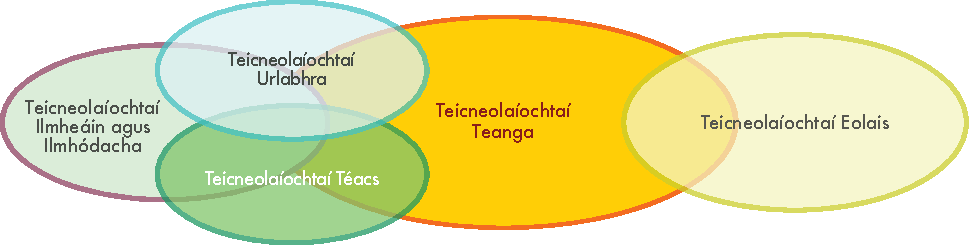
\includegraphics[width=\textwidth]{../_media/irish/language_technologies}
  \caption{Teicneolaíocht Teanga i gComhthéacs}
  \label{fig:ltincontext_de}
  \colorrule{grey3}{\textwidth}{1.5pt}
\end{figure*}

 Nuair a dhéanaimid cumarsáid, nascaimid teanga le modhanna eile cumarsáide agus meán faisnéise – mar shampla, tig le comharthaí agus gothaí gnúise bheith mar chuid de labhairt. Nascann téacs digiteach le pictiúir agus fuaimeanna. Tig le teanga i bhfoirm labhartha agus scríofa bheith i scannáin. I bhfocail eile, forluíonn teicneolaíochtaí labhartha agus téacs agus déanann siad idirghníomhú le teicneolaíochtaí eile a éascaíonn próiseáil cumarsáide ilmhódaí agus cáipéisí ilmheáin. 

Sna codanna seo a leanas, pléifimid na príomhréimsí feidhme de theicneolaíocht teanga, i.e. seiceáil teanga, cuardach gréasáin, teicneolaíocht labhartha agus uathaistriú. Áirítear anseo feidhmchláir agus bunteicneolaíochtaí cosúil le

\begin{itemize}
\item ceartú litrithe
\item tacaíocht údaraithe
\item foghlaim teanga ríomhchuidithe
\item aisghabháil faisnéise
\item baint faisnéise
\item achoimriú téacs
\item freagairt ceiste
\item aithint labhartha 
\item sintéis labhartha
\end{itemize}

Is réimse bhunaithe thaighde atá i dteicneolaíocht teanga agus sraith fhairsing litríochta ar fáil ina thaobh. Moltar don léitheoir a bhfuil suim aige ann na tagairtí seo a léamh: \cite{carstensen-etal1} \cite{jurafsky-martin01} \cite{manning-schuetze1} \cite{lt-world1} \cite{lt-survey1}. %NEEDS TO BE TRANSLATED

Sula bpléifimid na réimsí feidhme thuas, déanfaimid cur síos gairid ar ailtireacht an ghnáthchórais LT.

\subsection{Ailtireachtaí Feidhmchláir}

Is iondúil go mbíonn roinnt comhábhar i bhfeidhmchláir bogearraí do phróiseáil teanga a léiríonn gnéithe éagsúla den teanga. Léiríonn an fíor~\ref{fig:textprocessingarch_de} ailtireacht an-simplithe ar féidir a fháil i ngnáthchóras próiseála téacs. Laimhseálann an chéad trí mhodúl struchtúr agus brí an ionchuir téacs:

\begin{figure*}[htb]
  \colorrule{grey3}{\textwidth}{1.5pt}
  \center
  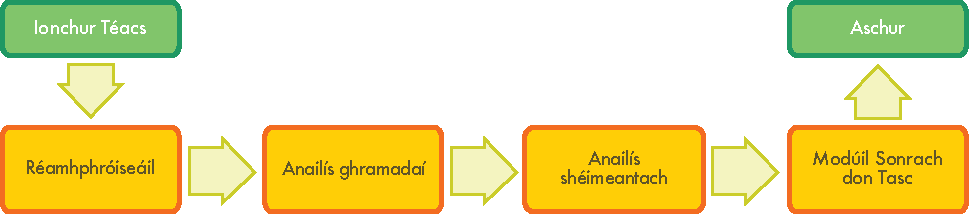
\includegraphics[width=\textwidth]{../_media/irish/text_processing_app_architecture}
  \caption{Ailtireacht Tipiciúil ar Fheidhmchlár Próiseála Téacs}
  \label{fig:textprocessingarch_de}
  \colorrule{grey3}{\textwidth}{1.5pt}
\end{figure*}

\begin{enumerate}
\item Réamhphróiseáil: glantar na sonraí, déantar anailís ar fhormáidiú nó baintear é, braitear an teanga ionchuir, ionadaítear giorrúcháin ``le'd thoil'' in ionad ``le do thoil'', agus mar sin de.
\item Anailís ghramadaí: aimsítear an briathar, a chuspóirí, mionathraitheoirí agus codanna eile den chaint mar aon le struchtúr na habairte a bhrath.
\item Anailís shéimeantach: déantar imdhealú débhríochta (i.e., ríomhtar brí chuí focal i gcomhthéacs ar leith); réitítear iarthagra (i.e., cé na forainmneacha a thagraíonn do na hainmfhocail san abairt) agus ionadaítear teilgean cainte; agus léirítear brí na habairte ar bhealach ar féidir leis an inneall é a léamh.
\end{enumerate}

Tar éis anailís a dhéanamh ar an téacs, tig le modúil tascshonracha feidhmeanna eile a dhéanamh, cosúil le huathachoimriú agus cuardaigh bhunachar sonraí. Is cur síos simplithe agus idéalaithe é seo ar an ailtireacht feidhme agus léiríonn sé castacht na bhfeidhmchlár LT.  

Tar éis na croíréimsí feidhmchláir a thabhairt isteach do theicneolaíocht teanga, tabharfaimid forbhreathnú gairid ar sheasamh na taighde LT agus an t-oideachas inniu, agus críochnóimid le forbhreathnú ar chláir taighde atá imithe agus atá ann faoi láthair. Ansin cuirfimid meastachán saineolach ar fáil do chroíuirlisí agus acmhainní LT i dtéarmaí na ndiminsean éagsúil cosúil le hinfhaighteacht, aibíocht agus caighdeán. Déantar achoimre ar staid ghinearálta an LT don Ghaeilge i dtábla ~\ref{fig:lrlttable_de}.


\subsection{Croíréimsí Feidhme} 

Sa chuid seo, dírimid ar na huirlisí agus acmhainní LT is tábhachtaí, agus tugaimid forbhreathnú ar ghníomhaíochtaí LT in Éirinn. Is féidir uirlisí agus acmhainní a bhfuil líne fúthu sa téacs a aimsiú chomh maith sa tábla ag deireadh na caibidle seo. 

\subsubsection{Seiceáil Teanga}

Tá a fhios ag gach duine a d’úsáid próiseálaí focal cosúil le Microsoft Word go bhfuil seiceálaí litrithe ann a léiríonn botúin litrithe agus a mholann ceartaithe. Chuir na chéad chláir um cheartú litrithe liosta focal aisbhainte i gcomparáid le foclóir focal atá litrithe i gceart. Inniu, tá na cláir seo i bhfad níos sofaisticiúla. Ag baint úsáide as algartaim theangaspleácha d’anailís téacs, braitheann siad earráide a bhaineann le moirfeolaíocht (e.g. foirmiú iolra) mar aon le hearráidí a bhaineann le comhréir, cosúil le briathar in easnamh nó coimhlint le comhaontú briathair-ainmní (e.g. she *write a letter). Ach ní bhfaigheadh formhór na seiceálaithe litrithe aon earráidí sa téacs seo \cite{zar1} a leanas: 

\begin{quote}
  I have a spelling checker,\\
  It came with my PC.\\
  It plane lee marks four my revue\\
  Miss steaks aye can knot sea.
\end{quote}

Caithfear anailís a dhéanamh ar an gcomhthéacs de ghnáth chun na cineálacha seo earráide a láimhseáil. Caithfidh an cineál seo anailíse tarraingt ar ghramadach theangashonrach atá códaithe go dian ag saineolaithe sna bogearraí nó ar mhúnla teanga staitistiúil. Sa chás seo, ríomhann múnla dóchúlacht focail áirithe de réir mar a thagann sé chun cinn in áit ar leith. Is féidir múnla teanga staitistiúil a chruthú go huathoibríoch trí líon mór sonraí teanga (ceart) a úsáid (ar a dtugtar corpas téacs). Forbraíodh formhór an dá chur chuige seo timpeall ar shonraí ón mBéarla. Faoi láthair, ní féidir le ceachtar cur chuige aistriú go héasca go Gaeilge mar níl mórán acmhainní teanga ar fáil cosúil le corpais téacs chun múnla staitistiúil a chur le chéile agus níl dóthain saineolais ann chun eolas teangeolaíoch a ionchódú de láimh i ngramadach.

\boxtext{Níl úsáid na seiceála teanga teoranta do phróiseálaithe focail; baineann sé chomh maith le córais tacaíochta údaraithe.} %NEEDS TO BE TRANSLATED

Níl seiceáil teanga teoranta do phróiseálaithe focail; úsáidtear chomh maith í i “gcórais tacaíochta údaraithe”, i.e. timpeallachtaí bogearraí ina scríobhtar lámhleabhair agus cáipéisíocht eile chuig caighdeáin speisialta do tháirgí coimpléascacha TF, cúraim shláinte, innealtóireachta agus eile. Tá imní ar chuideachtaí go ndéanfaidh custaiméirí gearáin faoi úsáid mhíchuí agus éilimh dhamáiste mar gheall ar threoracha nár thuig siad i gceart, tá siad ag díriú níos mó ar chaighdeán na cáipéisíochta teicniúla agus ag díriú ar an margadh idirnáisiúnta (trí aistriúchán nó logánú) ag an am céanna. De bharr dul chun cinn i bpróiseáil teanga nádúrtha, forbraíodh bogearraí tacaíochta údaraithe, a chuidíonn le scríbhneoir na cáipéisíochta teicniúla foclóir agus struchtúir abairte a úsáid atá comhsheasmhach le rialacha tionscail agus srianta téarmeolaíochta (corparáideach).

\begin{figure*}[htb]
  \colorrule{grey3}{\textwidth}{1.5pt}
  \center
  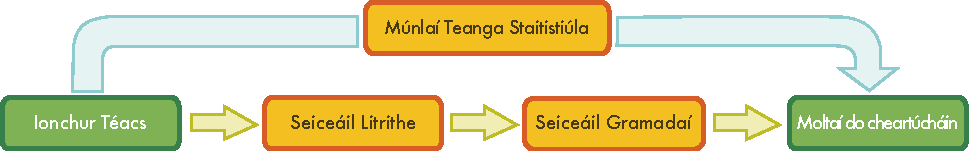
\includegraphics[width=\textwidth]{../_media/irish/language_checking}
  \caption{Seiceáil Teanga (ar chlé: riailbhunaithe; ar dheis: staistiúil)}
  \label{fig:langcheckingaarch_de}
  \colorrule{grey3}{\textwidth}{1.5pt}
\end{figure*}

Tá uirlisí seiceála teanga ar fail don Ghaeilge i sraitheanna oifige cosúil le Microsoft Office agus Open Office. Ní hamháin go seiceálann na huirlisí seo litriú ach seiceálann siad go leor gnéithe de ghramadach na Gaeilge, ach ní féidir iad a chomhtháthú go héasca le táirgí atá ann cheana i gcónaí. Mar shampla, ní dhéanann ach seiceálaí teanga amháin don Ghaeilge \cite{gramadoir} níos mó ná ceartú litrithe, agus ní féidir é a chomhtháthú go héasca faoi láthair le Open Office ná Microsoft Word (cé go bhfuil an obair seo ar siúl agus an cháipéis seo á scríobh). Maidir le ceartú litrithe, ní dhearnadh nuashonrú ar sheiceálaí litrithe Microsoft le blianta fada.  Níl ach seiceálaí litrithe amháin (Gaelspell http://borel.slu.edu/ispell/) a ndéantar nuashonrú seasta air, d’fhoinse oscailte agus ar fáil do Word/Ooo/Firefox, etc.

Seachas seiceálaithe litrithe agus tacaíocht údaraithe, tá seiceáil teanga tábhachtach chomh maith i réimse na foghlama teanga ríomhchuidithe. Agus ceartaíonn feidhmchláir seiceála teanga ceisteanna innill chuardaigh go huathoibríoch chomh maith, mar a aimsítear i moltaí \textit{Did you mean~\dots} de chuid Google.

\subsubsection{Cuardach Gréasáin}

Is é cuardach gréasáin, inlín nó leabharlainne digiteach an feidhmchláir teicneolaíochta teanga is mó a úsáidtear ach is tearcfhorbartha ar domhan. Láimhseálann inneall cuardaigh Google, a thosaigh i 1998, timpeall 80\% de gach cuardach agus os cionn 90\% den uile chuardach ó úsáideoirí idirlín in Éirinn \cite{googlemarketshare}.  Agus an cháipéis seo á scríobh, níl briathar oifigiúil i nGaeilge i gcomhair ``to google'' mar atá sa Ghearmáinis, mar shampla. Ach sa teanga choitianta, nuair a úsáidtear focail iasachta Bhéarla, úsáidtear an téarma ``gúgláil'' \cite{kilgarriff2010}.  Níor athraíodh comhéadan cuardaigh agus leathanach torthaí Google go suntasach ón gcéad leagan. Ach sa leagan reatha, cuireann Google ceartú litrithe ar fáil d’fhocail nár litríodh i gceart (ach ní don Ghaeilge) agus tá bunchumais chuardaigh shéimeantacha ionchorpraithe anois ar féidir leo cruinneas cuardaigh a fheabhsú trí anailís a dhéanamh ar théarmaí i gcomhthéacs an chuardaigh \cite[googlesemsearch]. Léiríonn scéal ratha Google gur féidir leis an líon mór sonraí atá ar fáil agus teicníochtaí innéacsaithe éifeachtúla torthaí sásúla a sheachadadh do chur chuige staitistiúil. 

\begin{figure*}[htb]
  \colorrule{grey3}{\textwidth}{1.5pt}
  \center
  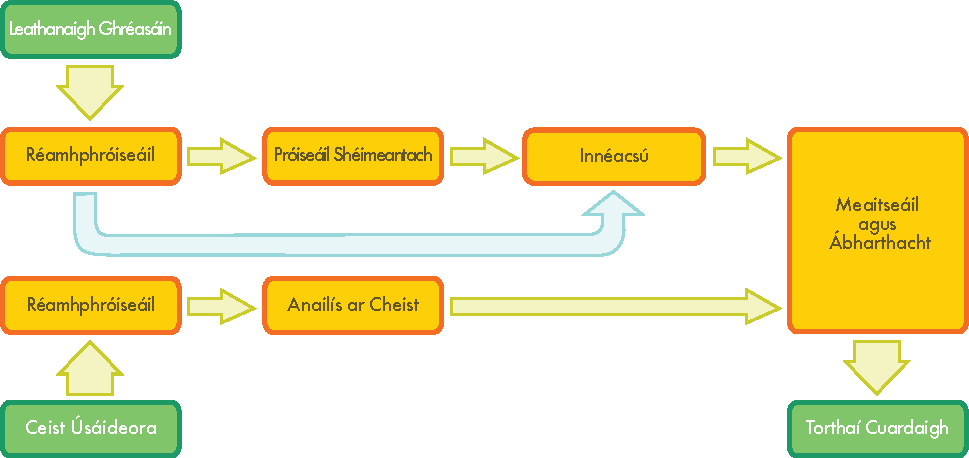
\includegraphics[width=\textwidth]{../_media/irish/web_search_architecture}
  \caption{Ailtireacht do Chuardach Gréasáin}
  \label{fig:websearcharch_de}
  \colorrule{grey3}{\textwidth}{1.5pt}
\end{figure*}

D’iarratais faisnéise níos sofaisticiúla , is gá eolas teangeolaíochta níos doimhne a chomhtháthú do \textbf{léirmhíniú téacs}. Léirigh trialacha ag úsáid \textbf{acmhainní foclóireachta} cosúil le teasárais nó acmhainní teanga ointeolaíocha (e.g. WordNet don Bhéarla nó Líonra Séimeantach na Gaeilge don Ghaeilge) feabhsúcháin ar leathanaigh a aimsiú ag úsáid chomhchiallaigh na dtéarmaí cuardaigh bunaigh, cosúil le \textit{fuinnimh adamach} [atomic energy], \textit{cumhacht núicléach} [nuclear energy], nó téarmaí eile a bhfuil baint éigin acu leis.

Beidh ar an gcéad ghlúin eile d’innill chuardaigh teicneolaíocht teanga níos sofaisticiúla a chur san áireamhm go háirithe d’fhonn déileáil le cuardaigh ina bhfuil ceist nó cineál abairte eile seachas liosta eochairfhocal. Don cheist, \textit{Tabhair liosta dom do na cuideachtaí ar fad ar ghlac cuideachtaí eile ceannas orthu le cúig bliana anuas} caithfidh an córas LT anailís a dhéanamh ar an abairt ó thaobh comhréire agus séimeantaigh mar aon le hinnéacs a chur ar fáil chun cáipéisí cuí a aimsiú go tapa. Teastóidh parsáil chomhréire do fhreagra sásúil chun anailís a dhéanamh ar struchtúr gramadaí na habairte agus cinneadh a dhéanamh go bhfuil an t-úsáideoir ag iarraidh cuideachtaí a glacadh, ní cuideachtaí a ghlac cuideachtaí eile. Don fhrása \textit{le cúig bliana anuas}, caithfidh an córas cinneadh a dhéanamh maidir leis na blianta ábhartha. Agus, caithfear an cheist a mheaitseáil le méid ollmhór sonraí neamhstruchtúrtha chun píosa nó píosaí eolais ábhartha a theastaíonn ón úsáideoir a fháil. Tugtar ``aisghabháil faisnéise'' air seo, agus baineann sé le cáipéisí ábhartha a chuardach agus a rangú. Chun liosta cuideachataí a chruthú, caithfidh an córas sraith focal ar leith sa cháipéis a aithint mar ainm cuideachta, próiseas ar a dtugtar ``aithint ainm aonáin''.

\boxtext{Beidh ar an gcéad ghlúin eile d’innill chuardaigh teicneolaíocht teanga níos sofaisticiúla a chur san áireamhm.}

Dúshlán níos déine is ea ceist a mheaistseáil i dteanga amháin le cáipéisí i dteanga eile. Baineann aisghabháil faisnéise trasteangaí  le ceist a uathaistriú sna teangacha foinse féideartha ar fad agus ansin na torthaí ar fad a aistriú ar ais go dtí an sprioctheanga. 

Anois agus sonraí á n-aimsiú i bhformáidí neamhthéacsúla, is gá go mbeadh seirbhísí chun aisghabháil faisnéise ilmheáin a sholathar trí íomhánna, comhaid fuaime agus sonraí físe a chuardach. I gcás comhad fuaime agus físe, caithfidh modúl aitheantais labhartha an t-ábhar labhartha a thiontú ina théacs (nó chuig léirmhíniú foghraíochta) ar féidir é a mheaitseáil in aghaidh ceist úsáideora.

 In Éirinn, cuireann líon beag soláthraithe cosúil le Maithú Teoranta agus grúpaí acadúla éagsúla teicneolaíochta teanga comhábhair ar fáil d’anailís foclóireachta agus tascanna cosúla a d’fhéadfaí a úsáid i gcuardach gréasáin. Tá inneall cuardaigh don Ghaeilge http://aimsigh.com, a dearadh don teanga (cuardaigh fréamhaithe etc.) ar fáil ó timpeall 2005-2006 ach deir an t-údar go bhfuil an tionscadal éagtha faoi láthair mar nár úsáideadh mórán é agus deir sé ``nach fiú infheistiú i dtaighde/forbairt ar na nithe seo mura n-úsáideann Gaeilgeoirí iad – tá siad sásta le Google.''  Dá bhrí sin, níl aon tionscadal/táirge innill chuardaigh Gaeilge ar scála mór faoi lathair seachas comhéadan Gaeilge Google atá logánaithe ach nach bhfuil optamaithe ná oiriúnaithe le hoibriú sa teanga.
  
\subsubsection{Teicneolaíocht Teanga}

Úsáidtear teicneolaíocht idirghníomhaíochta labhartha chun comhéadain a chruthú a chumasaíonn úsáideoirí le hidirghníomhú i dteanga labhartha in áit amharc grafach, méarchlár agus luchóg. Inniu, is gnách go n-úsáidtear na comhéadain úsáideora chainte (VUI) seo do sheirbhísí teileafóin cuid nó iomlán uathoibríoch a chuireann cuideachtaí ar fáil do chustaiméirí, fostaithe nó comhpháirtithe. Áirítear le fearainn ghnó a bhíonn ag brath go hiomlán ar VUIanna baincéireacht, slabhra soláthair, iompar poiblí agus teileachumarsáid. Áirítear le húsáidí eile de theicneolaíocht chainte comhéadain le córais treoshuímh cairr agus úsáid na teanga labhartha mar rogha mhalartach le comhéadain ghrafacha nó scáileán tadhaill ar ghutháin chliste.

\boxtext{Úsáidtear teicneolaíocht idirghníomhaíochta labhartha mar bhunús le comhéadain a chruthú a cheadaíonn úsáideoirí le hidirghníomhú le teanga labhartha in áit amharc grafach, méarchlár agus luchóg.}

\begin{figure*}[htb]
  \colorrule{grey3}{\textwidth}{1.5pt}
  \center 
  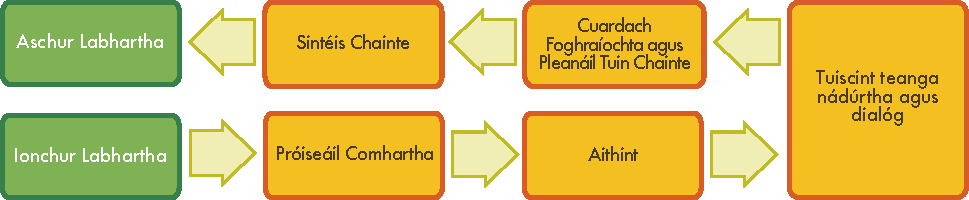
\includegraphics[width=\textwidth]{../_media/irish/simple_speech-based_dialogue_architecture}
  \caption{Ailtireacht Dialóige Simplí Labhairtbhunaithe}
  \label{fig:dialoguearch_de}
  \colorrule{grey3}{\textwidth}{1.5pt}
\end{figure*}

Tá ceithre theicneolaíocht i dteicneolaíocht labhartha:

\begin{enumerate}
\item \textbf {Aithint cainte} uathoibríoch (ASR) a chinneann cé na focail a deirtear i sraith ar leith fuaimeanna an úsáideora.
\item Déanann tuiscint teanga nádúrtha anailís ar struchtúr comhréir labhartha an úsáideora agus míníonn sí í de réir an chórais atá i gceist.
\item Cinneann bainistíocht dialóige cén gníomh le déanamh de réir ionchur an úsáideora agus fheidhmíocht an chórais.    
\item Aistríonn \textbf{sintéis chainte} (téacs go caint nó TTS) freagra an chórais ina fhuaimeanna don úsáideoir.
\end{enumerate}

Ar cheann de na mórdhúshláin a bhaineann le córais ASR na focail a deir úsáideoirí a aithint go beacht. Is é is ciall leis seo an réimse rudaí a deir an t-úsáideoir a shrianú chuig sraith theoranta eochairfhocal, nó múnlaí teanga a chruthú de láimh a chlúdaíonn réimse leathan teanga nádúrtha. Trí fheidhm a bhaint as teicníochtaí ríomhfhoghlama, is féidir múnlaí teanga a chothú ó chorpais chainte, i.e. bainiúcháin mhóra de chomhaid chainte fuaime agus tras-scríbhinní téacs. Nuair a chuirtear srian ar chaint, is éigean do dhaoine an comhéadan cainte úsáideora a úsáid ar bhealach docht agus déantar damáiste do ghlacadh úsáideora; ach ardófar costais go suntasach de bharr cruthú, tiúnáil agus cothabháil múnla teanga saibhre. Is iondúil go mbíonn VUIanna a úsáideann múnlaí teanga agus a cheadaíonn don úsáideoir a bhfuil i gceist acu a chur in iúl ar bhealach níos solúbtha – a thosaíonn le fáiltiú \textit{Conas is féidir liom cabhair leat?} – uathoibríoch agus glacann úsáideoirí níos fearr leo. 

Is iondúil go n-úsáideann cuideachta cainteoirí gairmiúla chun caint a réamhthaifeadadh chun aschur an chomhéadain úsáideora cainte a chruthú. Do chaint statach nach mbraitheann an fhoclaíocht ar chomhthéacsanna áirithe úsáidte nó sonraí úsáideora pearsanta, tig leis seo taithí níos saibhre a thabhairt don úsáideoir. Ach d’fhéadfadh ábhar níos dinimiciúla bheith beagán mínádúrtha mar gheall gur cuireadh comhaid fuaime randamacha le chéile. Tá córais TTS an lae inniu ag feabhsú (cé gur féidir barrfeabhas a chur orthu) maidir le caint dhinimiciúil nádúrtha a tháirgeadh. 

Rinneadh caighdeánú suntasach ar chomhéadain i margadh na teicneolaíochta labhartha le linn an chéid a caitheadh i dtéarmaí a gcomhábhair theicneolaíochta éagsúla. Bhí comhdhlúthú margaidh láidir in aithint cainte agus sintéis chainte chomh maith. Bhí cúigear imreoirí domhanda i gceannas ar na margaí naisiúnta G20 (tíortha athléimneacha ina bhfuil daonraí arda), le Nuance (S.A.M.) agus Loquendo (an Iodáil) ina n-imreoirí ceannasacha san Eoraip.  In 2011, d’fhógair Nuance gabháil Loquendo, a léiríonn céim eile i gcomhdhlúthú margaidh.

Tá sintéiseoirí agus aithneoirí ar fud na hÉireann trí roinnt tionscadal acadúil. Ach, agus an cháipéis seo á scríobh, nílimid ar an eolas maidir le haon fheidhmchláir thráchtála seachas roinnt uirlisí foghlama (a n-úsáideann an chuid is mó díobh codanna réamhthaifeadta seachas sintéis iomlán) a úsáideann teicneolaíochtaí cainte don Ghaeilge.

Ag féachaint chun tosaigh, tarlóidh athruithe suntasacha de bharr scaipeadh guthán cliste mar léibheann nua chun caidreamh custaiméara a bhainistiú anuas ar theileafóin sheasta, ar an Idirlíon agus ar an ríomhphost. Beidh tionchar aige seo ar an gcaoi a n-úsáidfear teicneolaíocht idirchaidrimh chainte. Don fhadtréimhse, beidh níos lú VUIanna teileafónbhunaithe agus beidh ról i bhfad níos lárnaí ag an teanga labhartha amhail ionchur soláimhsithe do ghutháin chliste. Tiománfaidh feabhsúcháin chéimnithe é seo go príomha i gcruinneas aithint cainte neamhspleách ar chainteoir trí sheirbhísí deachtúcháin a chuirtear ar fáil cheana mar sheirbhísí lárnaithe d’úsaideoirí guthán cliste.


\subsubsection{Uathaistriú}

Téann an smaoineamh maidir le ríomhairí digiteacha a úsáid le teangacha nádúrtha a aistriú siar go dtí 1946 agus tháinig maoiniú suntasach ina dhiaidh sin do thaighde sna 1950idí agus arís sna 1980idí. Ach fós féin, ní féidir le \textbf{huathaistriú} (``machine translation,'' MT) an rud a rabhthas ag súil uaidh a chomhlíonadh, is é sin uathaistriú cuimsitheach. 

\boxtext{Ag a leibhéal bunúsach, ionadaíonn Uathaistriú focail i dteanga nádúrtha amháin le focail i dteanga eile.}

Is é an cur chuige is bunúsaí le huathaistriúchán focail i dtéacs i dteanga nádúrtha amháin a ionadú go huathoibríoch le focail i dteanga eile. Tig leis seo bheith an-úsáideach i bhfearainn ainmní ina bhfuil teanga foirmleach an-srianta cosúil le tuairiscí aimsire. Ach, chun dea-aistriúchán a chur ar fáil do théacsanna nach bhfuil caighdeánaithe, caithfear aonaid téacs níos mó (frásaí, abairtí, nó pasáistí iomlána) a mheaitseáil lena macasamhail sa sprioctheanga. Is é an mórdheacracht go bhfuil teanga dhaonna débhríoch. Cruthaíonn débhríochas dúshláin ar il-leibhéil, cosúil le débhríochas focail ar leibhéal foclóireachta (is branda cairr nó ainmhí atá in \textit{jaguar}).

Bealach amháin le córas MT a thógáil is ea rialacha teangeolaíocha a úsáid. D’aistriúcháin idir teangacha le gaol gar eatarthu, d’fhéadfaí aistriúchán ionadaithe dhírigh a úsáid i gcásanna cosúil leis an sampla thuas. Ach, go minic déanann córais riailbhunaithe (nó eolasbhunaithe teangeolaíochta) anailís ar an téacs ionchuir agus cruthaíonn siad léiriú siombalach idirmheánach ónar féidir an téacs a chruthú sa sprioctheanga. Braitheann rath na modhanna seo ar infhaighteacht foclóirí fairsinge le faisnéis mhoirfeolaíochta, chomhréire agus shéimeantach, agus sraitheanna níos mó de rialacha gramadaí a dhear teangeolaithe oilte go cúramach. Is próiseas an-fhada agus dá bhrí sin, costasach atá anseo.

\begin{figure*}[htb]
  \colorrule{grey3}{\textwidth}{1.5pt}
  \center
  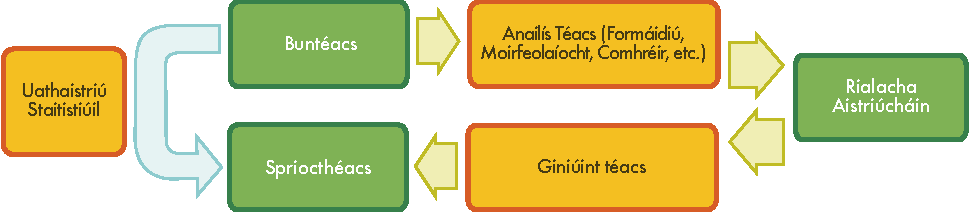
\includegraphics[width=\textwidth]{../_media/irish/machine_translation}
  \caption{Uathaistriú (ar chlé: staitistiúil, ar dheis: riailbhunaithe)}
  \label{fig:mtarch_de}
  \colorrule{grey3}{\textwidth}{1.5pt}
\end{figure*}

Go déanach sna 1980idí nuair a d’fheabhsaigh cumhacht ríomhaireachta agus a laghdaigh sé i gcostas, ach bhí suim níos mó i múnlaí staitistiúla d’uathaistriú. Eascraíonn múnlaí staitistiúla ó anailís a dhéanamh ar chorpais téacs dhátheangacha, cosúil le \textbf{corpais chomhthreomhara} Europarl, ina bhfuil imeachtaí Pharlaimint na hEorpa in 11 theanga Eorpacha. Má chuirtear dóthain sonraí ann, oibríonn MT staitistiúil sách maith chun míniú measta a bhaint as téacs i dteanga iasachta trí leaganacha comhthreomhara a phróiseáil agus pátrúin focail sochreidte a aimsiú. Ach, neamhchosúil le córais eolasbhunaithe, cruthaíonn MT staitistiúil (nó sonraíbhunaithe) aschur neamhghramadaí go minic. Tá buntáistí ag baint le MT sonraíbhunaithe mar nach dteastaíonn an oiread iarracht dhaonna, agus tig leis sonraíochtaí speisialta den teanga a chlúdach (e.g. leaganacha cainte) a dtugtar neamhaird orthu i gcórais eolasbhunaithe. 

Is iondúil go mbíonn na láidreachtaí agus na laigí atá ag uathaistriú eolasbhunaithe agus sonraíbhunaithe comhlántach, agus anois díríonn taighdeoirí ar chur chuige hibride a úsáideann an dá mhodheolaíocht. Úsáideann cur chuige amháin córais eolasbhunaithe agus sonraíbhunaithe mar aon le modúl roghnaithe a dhéanann cinneadh ar an aschur is fearr do gach abairt. Ach, ní bheidh torthaí d'abairtí níos faide ná 12 fhocal foirfe in aon chor. Réiteach níos fearr is ea na codanna is fearr do gach abairt as ilaschuir a cheangal; tig leis seo bheith réasúnta coimpléascach, mar nach mbíonn codanna comhfhreagracha de roghanna malartacha soiléir i gcónaí agus caithfear ailíniú a dhéanamh orthu. 

\boxtext{De bharr easpa sonraí, tá dúshlán ar leith ag baint le hUathaistriú don Ghaeilge.} 

Tá cumas mór fós ann do chaighdeán na gcóras MT a fheabhsú. Baineann na dúshláin le hacmhainní teanga a oiriúnú chuig fearainn ainmní nó réimse úsáideora, agus an teicneolaíocht a chomhtháthú ina shreabhadh oibre ina bhfuil bunachair théarmaí agus cuimhní aistriúcháin cheana. Fadhb eile is ea go bhfuil formhór na gcóras reatha bunaithe ar an mBéarla agus ní thacaíonn mórán acu le Gaeilge. Dá bharr seo bíonn frithchuimilt sa sreabhadh oibre aistriúcháin agus cuireann sé brú ar úsáideoirí MT uirlisí códaithe foclóireachta éagsúla a fhoghlaim do chórais éagsúla. 

Cuidíonn feachtais luachála comparáid a dhéanamh idir caighdeán na gcóras MT, an cur chuige éagsúil agus stádas na gcóras do phéirí teanga éagsúla. Léiríonn an tábla~\ref{fig:euromatrix_de} thíos, a réitíodh le linn thionscadal EC Euromatrix+, na feidhmíochtaí bunaithe ar phéirí a baineadh amach do 22 de na 23 teanga oifigiúil Eorpach. (Ní raibh an Ghaeilge san áireamh sa chomparáid de bharr easpa uirlisí bheith ar fáil.) Rangaíodh na torthaí de réir scór BLEU, a léiríonn scóir níos airde d’aistriúcháin níos fearr \cite{bleu1}. Gheobhadh aistritheoir daonna scór timpeall 80 pointe.

Baineadh amach na torthaí is fearr (i nglas agus gorm) i dteangacha a fhaigheann buntáiste as taighde suntasach i gcláir chomhordaithe agus ó na corpais chomhthreomhara a bhí ann (e.g. Béarla, Fraincis, Ollainnis, Spáinnis agus Gearmáinis). Léirítear na teangacha le torthaí níos measa i ndearg. Níl iarrachtaí forbartha ag na teangacha seo nó tá struchtúr an-difriúil acu ó na teangacha eile (e.g. Ungáiris, Máltais agus Fionlainnis).

\begin{figure*}[htbp]
  \centering
  \setlength{\tabcolsep}{0.17em}
  \small
  \begin{tabular}{>{\columncolor{corange1}}cccccccccccccccccccccccc}
    & \multicolumn{22}{>{\columncolor{corange1}}c}{Sprioctheanga -- \textcolor{grey1}{Target language}}\\\addlinespace[{-.009cm}] %NEEDS TO BE TRANSLATED
    \rowcolor{corange1}  & EN & BG & DE & CS & DA & EL & ES & ET & FI & FR & HU & IT & LT & LV & MT & NL & PL & PT & RO & SK & SL & SV\\
    EN & -- & \textcolor{blue}{40.5} & \textcolor{blue}{46.8} & \textcolor{green2}{52.6} & \textcolor{green2}{50.0} & \textcolor{blue}{41.0} & \textcolor{green2}{55.2} & \textcolor{purple}{34.8} & \textcolor{purple}{38.6} & \textcolor{green2}{50.1} & \textcolor{purple}{37.2} & \textcolor{green2}{50.4} & \textcolor{purple}{39.6} & \textcolor{blue}{43.4} & \textcolor{purple}{39.8} & \textcolor{green2}{52.3} & \textcolor{blue}{49.2} & \textcolor{green2}{55.0} & \textcolor{blue}{49.0} & \textcolor{blue}{44.7} & \textcolor{green2}{50.7} & \textcolor{green2}{52.0}\\
    BG & \textcolor{green}{61.3} & -- & \textcolor{purple}{38.7} & \textcolor{purple}{39.4} & \textcolor{purple}{39.6} & \textcolor{purple}{34.5} & \textcolor{blue}{46.9} & \textcolor{red3}{25.5} & \textcolor{red3}{26.7} & \textcolor{blue}{42.4} & \textcolor{red3}{22.0} & \textcolor{blue}{43.5} & \textcolor{red3}{29.3} & \textcolor{red3}{29.1} & \textcolor{red3}{25.9} & \textcolor{blue}{44.9} & \textcolor{purple}{35.1} & \textcolor{blue}{45.9} & \textcolor{purple}{36.8} & \textcolor{purple}{34.1} & \textcolor{purple}{34.1} & \textcolor{purple}{39.9}\\
    DE & \textcolor{green2}{53.6} & \textcolor{red3}{26.3} & -- & \textcolor{purple}{35.4} & \textcolor{blue}{43.1} & \textcolor{purple}{32.8} & \textcolor{blue}{47.1} & \textcolor{red3}{26.7} & \textcolor{red3}{29.5} & \textcolor{purple}{39.4} & \textcolor{red3}{27.6} & \textcolor{blue}{42.7} & \textcolor{red3}{27.6} & \textcolor{purple}{30.3} & \textcolor{red2}{19.8} & \textcolor{green2}{50.2} & \textcolor{purple}{30.2} & \textcolor{blue}{44.1} & \textcolor{purple}{30.7} & \textcolor{red3}{29.4} & \textcolor{purple}{31.4} & \textcolor{blue}{41.2}\\
    CS & \textcolor{green2}{58.4} & \textcolor{purple}{32.0} & \textcolor{blue}{42.6} & -- & \textcolor{blue}{43.6} & \textcolor{purple}{34.6} & \textcolor{blue}{48.9} & \textcolor{purple}{30.7} & \textcolor{purple}{30.5} & \textcolor{blue}{41.6} & \textcolor{red3}{27.4} & \textcolor{blue}{44.3} & \textcolor{purple}{34.5} & \textcolor{purple}{35.8} & \textcolor{red3}{26.3} & \textcolor{blue}{46.5} & \textcolor{purple}{39.2} & \textcolor{blue}{45.7} & \textcolor{purple}{36.5} & \textcolor{blue}{43.6} & \textcolor{blue}{41.3} & \textcolor{blue}{42.9}\\
    DA & \textcolor{green2}{57.6} & \textcolor{red3}{28.7} & \textcolor{blue}{44.1} & \textcolor{purple}{35.7} & -- & \textcolor{purple}{34.3} & \textcolor{blue}{47.5} & \textcolor{red3}{27.8} & \textcolor{purple}{31.6} & \textcolor{blue}{41.3} & \textcolor{red3}{24.2} & \textcolor{blue}{43.8} & \textcolor{red3}{29.7} & \textcolor{purple}{32.9} & \textcolor{red3}{21.1} & \textcolor{blue}{48.5} & \textcolor{purple}{34.3} & \textcolor{blue}{45.4} & \textcolor{purple}{33.9} & \textcolor{purple}{33.0} & \textcolor{purple}{36.2} & \textcolor{blue}{47.2}\\
    EL & \textcolor{green2}{59.5} & \textcolor{purple}{32.4} & \textcolor{blue}{43.1} & \textcolor{purple}{37.7} & \textcolor{blue}{44.5} & -- & \textcolor{green2}{54.0} & \textcolor{red3}{26.5} & \textcolor{red3}{29.0} & \textcolor{blue}{48.3} & \textcolor{red3}{23.7} & \textcolor{blue}{49.6} & \textcolor{red3}{29.0} & \textcolor{purple}{32.6} & \textcolor{red3}{23.8} & \textcolor{blue}{48.9} & \textcolor{purple}{34.2} & \textcolor{green2}{52.5} & \textcolor{purple}{37.2} & \textcolor{purple}{33.1} & \textcolor{purple}{36.3} & \textcolor{blue}{43.3}\\
    ES & \textcolor{green}{60.0} & \textcolor{purple}{31.1} & \textcolor{blue}{42.7} & \textcolor{purple}{37.5} & \textcolor{blue}{44.4} & \textcolor{purple}{39.4} & -- & \textcolor{red3}{25.4} & \textcolor{red3}{28.5} & \textcolor{green2}{51.3} & \textcolor{red3}{24.0} & \textcolor{green2}{51.7} & \textcolor{red3}{26.8} & \textcolor{purple}{30.5} & \textcolor{red3}{24.6} & \textcolor{blue}{48.8} & \textcolor{purple}{33.9} & \textcolor{green2}{57.3} & \textcolor{purple}{38.1} & \textcolor{purple}{31.7} & \textcolor{purple}{33.9} & \textcolor{blue}{43.7}\\
    ET & \textcolor{green2}{52.0} & \textcolor{red3}{24.6} & \textcolor{purple}{37.3} & \textcolor{purple}{35.2} & \textcolor{purple}{37.8} & \textcolor{red3}{28.2} & \textcolor{blue}{40.4} & -- & \textcolor{purple}{37.7} & \textcolor{purple}{33.4} & \textcolor{purple}{30.9} & \textcolor{purple}{37.0} & \textcolor{purple}{35.0} & \textcolor{purple}{36.9} & \textcolor{red3}{20.5} & \textcolor{blue}{41.3} & \textcolor{purple}{32.0} & \textcolor{purple}{37.8} & \textcolor{red3}{28.0} & \textcolor{purple}{30.6} & \textcolor{purple}{32.9} & \textcolor{purple}{37.3}\\
    FI & \textcolor{blue}{49.3} & \textcolor{red3}{23.2} & \textcolor{purple}{36.0} & \textcolor{purple}{32.0} & \textcolor{purple}{37.9} & \textcolor{red3}{27.2} & \textcolor{purple}{39.7} & \textcolor{purple}{34.9} & -- & \textcolor{red3}{29.5} & \textcolor{red3}{27.2} & \textcolor{purple}{36.6} & \textcolor{purple}{30.5} & \textcolor{purple}{32.5} & \textcolor{red2}{19.4} & \textcolor{blue}{40.6} & \textcolor{red3}{28.8} & \textcolor{purple}{37.5} & \textcolor{red3}{26.5} & \textcolor{red3}{27.3} & \textcolor{red3}{28.2} & \textcolor{purple}{37.6}\\
    FR & \textcolor{green}{64.0} & \textcolor{purple}{34.5} & \textcolor{blue}{45.1} & \textcolor{purple}{39.5} & \textcolor{blue}{47.4} & \textcolor{blue}{42.8} & \textcolor{green}{60.9} & \textcolor{red3}{26.7} & \textcolor{purple}{30.0} & -- & \textcolor{red3}{25.5} & \textcolor{green2}{56.1} & \textcolor{red3}{28.3} & \textcolor{purple}{31.9} & \textcolor{red3}{25.3} & \textcolor{green2}{51.6} & \textcolor{purple}{35.7} & \textcolor{green}{61.0} & \textcolor{blue}{43.8} & \textcolor{purple}{33.1} & \textcolor{purple}{35.6} & \textcolor{blue}{45.8}\\
    HU & \textcolor{blue}{48.0} & \textcolor{red3}{24.7} & \textcolor{purple}{34.3} & \textcolor{purple}{30.0} & \textcolor{purple}{33.0} & \textcolor{red3}{25.5} & \textcolor{purple}{34.1} & \textcolor{red3}{29.6} & \textcolor{red3}{29.4} & \textcolor{purple}{30.7} & -- & \textcolor{purple}{33.5} & \textcolor{red3}{29.6} & \textcolor{purple}{31.9} & \textcolor{red2}{18.1} & \textcolor{purple}{36.1} & \textcolor{red3}{29.8} & \textcolor{purple}{34.2} & \textcolor{red3}{25.7} & \textcolor{red3}{25.6} & \textcolor{red3}{28.2} & \textcolor{purple}{30.5}\\
    IT & \textcolor{green}{61.0} & \textcolor{purple}{32.1} & \textcolor{blue}{44.3} & \textcolor{purple}{38.9} & \textcolor{blue}{45.8} & \textcolor{blue}{40.6} & \textcolor{red3}{26.9} & \textcolor{red3}{25.0} & \textcolor{red3}{29.7} & \textcolor{green2}{52.7} & \textcolor{red3}{24.2} & -- & \textcolor{red3}{29.4} & \textcolor{purple}{32.6} & \textcolor{red3}{24.6} & \textcolor{green2}{50.5} & \textcolor{purple}{35.2} & \textcolor{green2}{56.5} & \textcolor{purple}{39.3} & \textcolor{purple}{32.5} & \textcolor{purple}{34.7} & \textcolor{blue}{44.3}\\
    LT & \textcolor{green2}{51.8} & \textcolor{red3}{27.6} & \textcolor{purple}{33.9} & \textcolor{purple}{37.0} & \textcolor{purple}{36.8} & \textcolor{red3}{26.5} & \textcolor{red3}{21.1} & \textcolor{purple}{34.2} & \textcolor{purple}{32.0} & \textcolor{purple}{34.4} & \textcolor{red3}{28.5} & \textcolor{purple}{36.8} & -- & \textcolor{blue}{40.1} & \textcolor{red3}{22.2} & \textcolor{purple}{38.1} & \textcolor{purple}{31.6} & \textcolor{purple}{31.6} & \textcolor{red3}{29.3} & \textcolor{purple}{31.8} & \textcolor{purple}{35.3} & \textcolor{purple}{35.3}\\
    LV & \textcolor{green2}{54.0} & \textcolor{red3}{29.1} & \textcolor{purple}{35.0} & \textcolor{purple}{37.8} & \textcolor{purple}{38.5} & \textcolor{red3}{29.7} & \textcolor{red2}{8.0} & \textcolor{purple}{34.2} & \textcolor{purple}{32.4} & \textcolor{purple}{35.6} & \textcolor{red3}{29.3} & \textcolor{purple}{38.9} & \textcolor{purple}{38.4} & -- & \textcolor{red3}{23.3} & \textcolor{blue}{41.5} & \textcolor{purple}{34.4} & \textcolor{purple}{39.6} & \textcolor{purple}{31.0} & \textcolor{purple}{33.3} & \textcolor{purple}{37.1} & \textcolor{purple}{38.0}\\
    MT & \textcolor{green}{72.1} & \textcolor{purple}{32.2} & \textcolor{purple}{37.2} & \textcolor{purple}{37.9} & \textcolor{purple}{38.9} & \textcolor{purple}{33.7} & \textcolor{blue}{48.7} & \textcolor{red3}{26.9} & \textcolor{red3}{25.8} & \textcolor{blue}{42.4} & \textcolor{red3}{22.4} & \textcolor{blue}{43.7} & \textcolor{purple}{30.2} & \textcolor{purple}{33.2} & -- & \textcolor{blue}{44.0} & \textcolor{purple}{37.1} & \textcolor{blue}{45.9} & \textcolor{purple}{38.9} & \textcolor{purple}{35.8} & \textcolor{blue}{40.0} & \textcolor{blue}{41.6}\\
    NL & \textcolor{green2}{56.9} & \textcolor{red3}{29.3} & \textcolor{blue}{46.9} & \textcolor{purple}{37.0} & \textcolor{blue}{45.4} & \textcolor{purple}{35.3} & \textcolor{blue}{49.7} & \textcolor{red3}{27.5} & \textcolor{red3}{29.8} & \textcolor{blue}{43.4} & \textcolor{red3}{25.3} & \textcolor{blue}{44.5} & \textcolor{red3}{28.6} & \textcolor{purple}{31.7} & \textcolor{red3}{22.0} & -- & \textcolor{purple}{32.0} & \textcolor{blue}{47.7} & \textcolor{purple}{33.0} & \textcolor{purple}{30.1} & \textcolor{purple}{34.6} & \textcolor{blue}{43.6}\\
    PL & \textcolor{green}{60.8} & \textcolor{purple}{31.5} & \textcolor{blue}{40.2} & \textcolor{blue}{44.2} & \textcolor{blue}{42.1} & \textcolor{purple}{34.2} & \textcolor{blue}{46.2} & \textcolor{red3}{29.2} & \textcolor{red3}{29.0} & \textcolor{blue}{40.0} & \textcolor{red3}{24.5} & \textcolor{blue}{43.2} & \textcolor{purple}{33.2} & \textcolor{purple}{35.6} & \textcolor{red3}{27.9} & \textcolor{blue}{44.8} & -- & \textcolor{blue}{44.1} & \textcolor{purple}{38.2} & \textcolor{purple}{38.2} & \textcolor{purple}{39.8} & \textcolor{blue}{42.1}\\
    PT & \textcolor{green}{60.7} & \textcolor{purple}{31.4} & \textcolor{blue}{42.9} & \textcolor{purple}{38.4} & \textcolor{blue}{42.8} & \textcolor{blue}{40.2} & \textcolor{green}{60.7} & \textcolor{red3}{26.4} & \textcolor{red3}{29.2} & \textcolor{green2}{53.2} & \textcolor{red3}{23.8} & \textcolor{green2}{52.8} & \textcolor{red3}{28.0} & \textcolor{purple}{31.5} & \textcolor{red3}{24.8} & \textcolor{blue}{49.3} & \textcolor{purple}{34.5} & -- & \textcolor{purple}{39.4} & \textcolor{purple}{32.1} & \textcolor{purple}{34.4} & \textcolor{blue}{43.9}\\
    RO & \textcolor{green}{60.8} & \textcolor{purple}{33.1} & \textcolor{purple}{38.5} & \textcolor{purple}{37.8} & \textcolor{blue}{40.3} & \textcolor{purple}{35.6} & \textcolor{green2}{50.4} & \textcolor{red3}{24.6} & \textcolor{red3}{26.2} & \textcolor{blue}{46.5} & \textcolor{red3}{25.0} & \textcolor{blue}{44.8} & \textcolor{red3}{28.4} & \textcolor{red3}{29.9} & \textcolor{red3}{28.7} & \textcolor{blue}{43.0} & \textcolor{purple}{35.8} & \textcolor{blue}{48.5} & -- & \textcolor{purple}{31.5} & \textcolor{purple}{35.1} & \textcolor{purple}{39.4}\\
    SK & \textcolor{green}{60.8} & \textcolor{purple}{32.6} & \textcolor{purple}{39.4} & \textcolor{blue}{48.1} & \textcolor{blue}{41.0} & \textcolor{purple}{33.3} & \textcolor{blue}{46.2} & \textcolor{red3}{29.8} & \textcolor{red3}{28.4} & \textcolor{purple}{39.4} & \textcolor{red3}{27.4} & \textcolor{blue}{41.8} & \textcolor{purple}{33.8} & \textcolor{purple}{36.7} & \textcolor{red3}{28.5} & \textcolor{blue}{44.4} & \textcolor{purple}{39.0} & \textcolor{blue}{43.3} & \textcolor{purple}{35.3} & -- & \textcolor{blue}{42.6} & \textcolor{blue}{41.8}\\
    SL & \textcolor{green}{61.0} & \textcolor{purple}{33.1} & \textcolor{purple}{37.9} & \textcolor{blue}{43.5} & \textcolor{blue}{42.6} & \textcolor{purple}{34.0} & \textcolor{blue}{47.0} & \textcolor{purple}{31.1} & \textcolor{red3}{28.8} & \textcolor{purple}{38.2} & \textcolor{red3}{25.7} & \textcolor{blue}{42.3} & \textcolor{purple}{34.6} & \textcolor{purple}{37.3} & \textcolor{purple}{30.0} & \textcolor{blue}{45.9} & \textcolor{purple}{38.2} & \textcolor{blue}{44.1} & \textcolor{purple}{35.8} & \textcolor{purple}{38.9} & -- & \textcolor{blue}{42.7}\\
    SV & \textcolor{green2}{58.5} & \textcolor{red3}{26.9} & \textcolor{blue}{41.0} & \textcolor{purple}{35.6} & \textcolor{blue}{46.6} & \textcolor{purple}{33.3} & \textcolor{blue}{46.6} & \textcolor{red3}{27.4} & \textcolor{purple}{30.9} & \textcolor{purple}{38.9} & \textcolor{red3}{22.7} & \textcolor{blue}{42.0} & \textcolor{red3}{28.2} & \textcolor{purple}{31.0} & \textcolor{red3}{23.7} & \textcolor{blue}{45.6} & \textcolor{purple}{32.2} & \textcolor{blue}{44.2} & \textcolor{purple}{32.7} & \textcolor{purple}{31.3} & \textcolor{purple}{33.5} & --\\
    \end{tabular}
  \caption{Uathaistriú idir 22 Theanga AE -- \textcolor{grey1}{Machine translation between 22 EU-languages \cite{euro1}}} 
  \label{fig:euromatrix_de}
\end{figure*}

\subsection{Réimsí Eile Feidhme}

Baineann réimse fothascanna nach bhfeictear ag leibhéal na hidirghníomhaíochta leis an úsáideoir i gcónaí, le feidhmchláir teicneolaíochta teanga a thógáil, ach cuireann siad feidhmeanna seirbhíse suntasacha “laistigh” den chóras atá i gceist. Bíonn siad ar fad mar chuid de shaincheisteanna taighde atá fásta anois ina bhfodhisciplíní aonair de theangeolaíocht ríomhaireachta. 

\boxtext{Cuireann feidhmchláir teicneolaíochta teanga feidhmeanna seirbhíse suntasacha ar fáil “laistigh” de chórais bhogearraí níos mó.}

Is réimse taighde ghníomhaigh atá i bhfreagairt ceisteanna, mar shampla, lenar tógadh corpais anótáilte agus lenar tosaíodh comórtais eolaíochta. Téann coincheap freagairte ceisteanna níos faide ná cuardaigh bunaithe ar eochairfhocail (ina bhfreagraíonn an t-inneall cuardaigh trí bhailiúchán cáipéisí a d’fhéadfadh bheith ábhartha a sheachadadh) agus a chumasaíonn úsáideoirí ceist a chur agus go dtugann an córas freagra amháin air. Mar shampla:

\textit{Ceist: Cén aois a bhí Neil Armstrong nuair a sheas sé ar an ngealach?}\\
\textit{Freagra: 38.}

Cé go bhfuil gaol ag freagairt ceisteanna le croíréimse an chuardaigh ghréasáin, is brat-téarma é seo anois ar shaincheisteanna taighde den chineál seo maidir leis na cineálacha éagsúla ceisteanna atá ann, agus an chaoi ar cheart iad a láimhseáil; conas anailís agus comparáid a dhéanamh ar shraith cáipéisí ina bhféadfadh an freagra a bheith (an dtugann siad freagraí coimhlinte?); agus an chaoi ar féidir eolas ar leith (an freagra) a bhaint i gceart as cáipéis gan neamhaird a thabhairt ar an gcomhthéacs. 

Bhain sé seo ina dhiaidh sin le baint faisnéise (IE), réimse a raibh an-tóir air agus a raibh tionchar aige nuair a chuaigh teangeolaíocht ríomhaireachta i dtreo staitistiúil ag tús na 1990idí. Díríonn IE ar phíosaí ar leith faisnéise a aithint i gcineálacha áirithe cáipéisí, cosúil le príomhpháirtithe i ngabhálacha cuideachta a aithint amhail a tuairiscíodh iad i scéalta nuachtáin. Cás coitianta eile a ndearnadh staidéar air is ea tuairiscí ar eachtraí sceimhlitheoireachta. Is í an fhadhb anseo an téacss a léarscáiliú chuig teimpleád a leagann amach déantóir na hoibre, sprioc, am, láthair agus torthaí na heachtra. Tá líonadh teimpléid fearainnshonrach ina shaintreith lárnach de IE, atá ina shampla eile de theicneolaíocht ``laistigh'' atá ina chuid de réimse taighde dea-chríochaithe a chaithfear bheith leabaithe i dtimpeallacht feidhmchláir oiriúnaigh i gcleachtadh.

Is dhá réimse teorann iad achoimriú agus \textbf{giniúint téacs} ar féidir leo feidhmiú mar fheidhmchláir astu féin nó ról tacaíochta bheith acu ``laistigh''. Déantar iarracht le hachoimriú na nithe is ríthábhachtaí as téacs fada a thabhairt i leagan gearr, agus ta sé ar cheann de na gnéithe atá ar fáil in Microsoft Word.  Úsáideann sé cur chuige staitistiúil den chuid is mó chun na focail ``thábhachtacha'' i dtéacs a shainaithint (i.e. focail a fheictear go minic sa téacs atá i gceist ach nach mbíonn chomh minic i ngnáthúsáid teanga) agus cinneadh a dhéanamh maidir leis na habairtí ina bhfuil na focail is ``tábhachtaí''. Ansin, baintear amach na habairtí seo agus cuirtear le chéile iad chun achoimre a chruthú. Is cás tráchtála an-choitianta é seo, níl in achoimriú ach saghas bainte abairtí, agus laghdaítear an téacs chuig foshraith a abairtí. Cur chuige malartach, ar a ndearnadh roinnt taighde, is ea chun branda nua abairtí a ghiniúint nach bhfuil ar fáil sa bhuntéacs. Tá tuiscint níos doimhne ag teastáil ar an téacs dó seo, agus dá bharr seo níl an cur chuige seo chomh láidir. Ar an iomlán, is annamh a úsáidtear ginteoir téacs mar fheidhmchlár as féin ach bíonn sé leabaithe i dtimpeallacht bogearraí níos mó cosúil le córas faisnéise cliniciúil a bhailíonn, a stórálann agus a phrósealann sonraí othair.  Níl i gcruthú tuairiscí ach ceann de na feidhmeanna d’achoimriú téacs.  

Don Ghaeilge, níl an oiread forbartha déanta ar na teicneolaíochtaí téacs seo is atá do theangacha Eorpacha eile. Díríodh ar fhreagairt ceisteanna, baint faisnéise agus achoimriú i roinnt comórtais oscailte i S.A.M. ó na 1990idí, á n-eagrú go príomha ag eagraíochtaí uarraithe ag an rialtas DARPA agus NIST. D’fheabhsaigh na comórtais seo an teicneolaíocht úrscothach, ach dhírigh siad den chuid is mó ar an mBéarla. Mar thoradh, níl na corpais anótáilte agus acmhainní speisialta eile a theastaíonn chun na tascanna seo a dhéanamh i dteangacha eile forbartha chomh maith. Cé go bhfuil roinnt ar fáil do theangacha Eorpacha le hacmhainní níos fearr cosúil leis an nGearmáinis, níl mórán uirlisí ná acmhainní riachtanacha ar fáil don Ghaeilge.

\subsection{Tionscal agus Cláir LT}

Tá tionscail úsáideora agus soláthróra ar fáil do LT Gaeilge ach díríonn siad go príomha ar sheirbhísí logánaithe agus aistrithe mar thoradh ar Acht na dTeangacha Oifigiúla agus bheith ina teanga oifigiúil san AE. Tá margadh i mbéal fáis chomh maith ann in oideachas de réir mar a thugann cleachtas múinteoireachta teicneolaíochtaí nua san áireamh. Ar an dóigh chéanna, tá treocht ag teacht chun cinn i measc na glúine níos óige i dtreo an ghá le tacaíocht LT fheabhsaithe don Ghaeilge.

Is fostóir suntasach atá sa tionscal teanga in Éirinn. Ag fás ó timpeall 4-5k post i lár na 90idí go dtí os cionn 12k ag tús an chéid seo, tá stop leis an bhfás anois agus timpeall 14--16k post díreach ar fáil sa tionscal logánaithe agus aistriúcháin in Éirinn.

Tá roinnt ionaid bharrfeabhais do theangeolaíocht agus taighde ar theicneolaíocht teanga agus forbairt tionscail, mar shampla tá oifigí ag Microsoft, IBM agus Symantec ar fad in Éirinn agus iad ag oibriú ar ghnéithe áirithe de LT. Ach ní dhéanann siad ach fíorbheagán oibre ar shonraí na Gaeilge.

Tá roinnt SMEanna tagtha chun tosaigh agus iad ag táirgeadh, mar shampla, feidhmchláir foclóra shoghluaiste don Ghaeilge. De réir mar a fhásann margaí soghluaiste agus an ghréasáin shóisialta, beidh níos mó deiseanna ag gnólachtaí chun teicneolaíocht teanga a sholáthar don Ghaeilge.

In ainneoin na bhfigiúirí láidre fostaíochta i dtionscal na teanga in Éirinn agus deiseanna atá ag fás sa mhargadh dúchais don teanga náisiúnta, bíonn formhór na hoibre in LT ``i bhfolach'' ón úsáideoir/gcustaiméar. Déarfadh do leor daoine gur mar is ceart dó bheith, mar is teicneolaíocht chumasaithe atá in LT a chuireann comhábhair ar fáil chun an chaoi a ndéanaimid idirghníomhaíocht le táirgí agus seirbhísí eile a shimpliú, a fheabhsú nó a réabhlóidiú. Mar shampla, ní smaoinimid ar na rudaí a tharlaíonn in inneall an chairr, bímid sásta go n-oibríonn siad. Ach, cruthaíonn an cás seo a dheacracht féin dúinn i bpobal an LT sa chaoi is go mbíonn sé deacair na buntáistí agus éilimh ar theicneolaíochtaí teanga a chur in iúl do go leor grúpaí. Dá bharr seo, éiríonn an cás nach bhfeiceann go leor daoine a oibríonn i réimsí gaolmhara an buntáiste a bhaineann le LT a úsáid ina réimse. 

Níl an margadh do theicneolaíochtaí teanga Gaeilge ach ag teacht chun tosaigh anois. I bpáirt, tá sé ag teacht ón teicneolaíocht teanga/sholáthróirí agus úsáideoirí seirbhíse aibí atá ann cheana, ach chomh maith ón éileamh atá á chothú ag cainteoirí Gaeilge ``uirbeacha''. Tá sé seo á éascú ag an mborradh ollmhór in TFC in Éirinn agus feabhsúcháin a rinneadh le déanaí i mbonneagar chun é seo a thacú. Tá sé de bharr, chomh maith, an bhorrtha atá ar ghníomhaíochtaí ar líne, líonrú sóisialta agus gníomhaíocht foghlama go háirithe, sa ghlúin níos óige a úsáideann an teanga beagnach gach lá agus a ghlacann léi na teicneolaíochtaí seo go luath ina nósanna maireachtála.


\subsection{Taighde agus Oideachas LT in Éirinn}

 Tá Éire mar bhaile do roinnt institiúidí ceannródaíocha taighde i réimse na teangeolaíochta ríomhaireahcta, agus tá an tIonad Náisiúnta do Theicneolaíocht Teanga suite in Ollscoil Chathair Bhaile Átha Cliath mar aon leis an Ionad do Logánú don Chéad Ghlúin Eile, a oibríonn ar theangeolaíocht ríomhaireachta a úsáid chun breisluach a thabhairt chuig domhandú, logánú agus rochtain faisnéise. Tá an dá ionad seo fadhbhunaithe agus tá naisc láidre acu le Taighde agus Forbairt thionsclaíoch go háitiúil agus thar lear, mar aon le naisc láidre le hionaid bharrfeabhais Eorpacha eile sa réimse. Tá an fhoireann uathaistrithe bunaithe ag an CNGL i measc na gceann is mó agus is rathúla ar domhan. Leis an saineolas seo ar fáil in institiúidí Éireannacha, is mór an t-iontas nach bhfuil an cás do theicneolaíochtaí teanga don Ghaeilge níos fearr. 

Ach, faoi láthair níl ach fochéim amháin ar fáil i dteangeolaíocht ríomhaireachta in ollscoileanna na hÉireann. Ní ghlacann an cúrsa céime seo ach le 25 mac léinn sa bhliain, agus cuirtear béim ar an nGaeilge i 5 áit díobh. De bharr nach bhfuil ach líon beag céimithe oilte go cuí ag dul isteach sa lucht saothair ón gcóras oideachais in Éirinn, ní haon ionadh go bhfuil an obair a dhéantar ag ionaid taighde Éireannacha níos suntasaí do theangacha eile ná mar atá don Ghaeilge.

Tá an pobal teangeolaíochtaí ríomhaireachta agus teicneolaíochta teanga in Éirinn réasúnta beag ach tá sé gníomhach. Tá go leor idirghníomhaíochta agus comhoibrithe idir institiúidí agus comhpháirtithe tionscail d'fhonn an réimse in Éirinn a choinneáil beo. Ach, seachas imeachtaí sna hionaid a luadh agus roinnt imeachtaí ollscoile, níl aon chomhdháil nó imeacht pobail don LT Gaeilge.


\subsection{Infhaighteacht Uirlisí agus Acmhainní}

Déantar achoimre sa tábla a leanas ar staid reatha na tacaíochta don teicneolaíocht teanga don Ghaeilge. Chuir saineolaithe sa réimse oibre an rátáil ar fáil do na huirlisí agus acmhainní reatha a chuir meastacháin ar fáil bunaithe ar scála ó 0 (an-íseal) go 6 (an-ard) de réir seacht gcritéar.

\begin{figure*}[htb]
  \centering
\begin{tabular}{>{\columncolor{orange1}}p{.33\linewidth}@{\hspace*{6mm}}c@{\hspace*{6mm}}c@{\hspace*{6mm}}c@{\hspace*{6mm}}c@{\hspace*{6mm}}c@{\hspace*{6mm}}c@{\hspace*{6mm}}c}
  \rowcolor{orange1}
   \cellcolor{white}&\begin{sideways}\makecell[l]{Méid}\end{sideways}%NEED TO TRANSLATE
  &\begin{sideways}\makecell[l]{\makecell[l]{Infhaighteacht} }\end{sideways} &\begin{sideways}\makecell[l]{Caighdeán}\end{sideways}
  &\begin{sideways}\makecell[l]{Clúdach}\end{sideways} &\begin{sideways}\makecell[l]{Aibíocht}\end{sideways} &\begin{sideways}\makecell[l]{Inbhuanaitheacht}\end{sideways} &\begin{sideways}\makecell[l]{Inoiriúnaitheacht}\end{sideways} \\ \addlinespace
  \multicolumn{8}{>{\columncolor{orange2}}l}{Teicneolaíocht Teanga: Uirlisí, Teicneolaíochtaí agus Feidhmchláir} \\\addlinespace
  Aithint cainte &5&1&3&2&4&3&3 \\ \addlinespace
  Sintéis Chainte &5&3&3&2&4&3&3\\ \addlinespace
  Anailís ghramadaí &4&2.5&2&2&4&2.5&2.5\\ \addlinespace
  Anailís shéimeantach &2&2&0&0&2&2&1\\ \addlinespace
  Giniúint téacs &2&1&2&2&2&1&2\\ \addlinespace
  Uathaistriú &5&3&1&1&4&1&2\\ \addlinespace
  \multicolumn{8}{>{\columncolor{orange2}}l}{Acmhainní Teanga: Acmhainní, Sonraí agus Bunachair Eolais} \\\addlinespace
  Corpais téacs &3&2&1&1&4&4&2.5\\ \addlinespace
  Corpais chainte &3&1&2&1&3&3&2\\ \addlinespace
  Corpais chomhthreomhara &2&1&2&1&2&2&1\\ \addlinespace
  Acmhainní foclóireachta &3&2.5&2&2&4&4&2.5\\ \addlinespace
  Gramadach &3&2&1&2&3&2&1\\
  \end{tabular}
  \caption{Bail thacaíocht na teicneolaíochta teanga don Ghaeilge}
  \label{fig:lrlttable_de}
\end{figure*}

Is féidir achoimre a dhéanamh ar na príomhthorthaí don Ghaeilge mar seo a leanas:

\begin{itemize}
\item Níl mórán uirlisí ná acmhainní ar fáil don Ghaeilge.
\item Is saincheisteanna atá i gcaighdeán, méid agus infhaighteacht do theicneolaíocht teanga don Ghaeilge. Nuair a bhíonn uirlisí ar fáil, is iondúil go mbíonn siad go maith ach níl mórán díobh ann agus níl siad ar fáil go forleathan. Os a choinne sin, san áit a mbíonn siad ar fáil go forleathan is iondúil go mbíonn an caighdeán níos ísle nó úsáidtear iad d’fhearann nó tasc ar leith.
\item Bíonn na huirlisí atá ann astu féin, cé go mbíonn siad d’ardchaighdeán. Go minic, ní bhíonn ach córas amháin ann do thasc ar leith, a chuireann srian ar roghanna.
\item Níl go leor de na hacmhainní ar fáil go héasca nó ní féidir iad a oiriúnú go héasca do thascanna nua.
\item Is cosúil go bhfuil taighde ar phróiseáil teanga ag céim bhreisithe i gcomparáid le reimsí eile cosúil le próiseáil téacs agus múnlú teanga in ainneoin go bhfuil bunuirlisí téacs ar fáil don Ghaeilge i roinnt feidhmchláir thráchtála. Léireodh sé seo go bhfuil éileamh ar bhunuirlisí mar seo de chaighdeán níos ísle fós.
\item D'ainneoin infhaighteacht acmhainní maithe do phróiseáil labhartha, mar shampla, tá srian ar an réimse seo de bharr droch-infhaighteacht, clúdach agus sonraí neamh-inbhuanaithe.
\item Tá bearna mhór i sonraí le húsáid le huirlisí teanga.	
\item Tá easpa croí-chomhábhair teicneolaíochta don Ghaeilge a chumasódh próiseáil teanga níos sofaisticiúla a theastaíonn chun feidhmchláir choimpléascacha a thógáil.
\item Tá bunuirlisí agus acmhainní anailíse focal dea-chaighdeáin ar fáil ach níl mórán de na huirlisí seo ann agus ní féidir iad a oiriúnú.
\end{itemize}

Léiríonn na torthaí go bhfuil tacaíocht teicneolaíochta theoranta ann don Ghaeilge agus go bhfuil na bunacmhainní teangeolaíochta le tacú le forbairt na gcroítheicneolaíochtaí in easnamh den chuid is mó. Is léir gur féidir na uirlisí seo a chruthú nuair a dhéantar infheistíocht sna huirlisí agus sna hacmhainní seo. Ach is cosúil go bhfuil moill ar dhul chun cinn de bharr easpa treorach i bhforbairt na n-uirlisí agus na n-acmhainní seo.

\subsection{Comparáid trasteanga}

Athraíonn staid reatha tacaíocht LT go mór ó phobal teanga amháin go pobal eile. D'fhonn comparáid a dhéanamh idir teangacha, cuirfear os bhur gcomhair sa chuid seo measúnú bunaithe ar dhá réimse feidhme samplacha (uathaistriúchán agus próiseáil cainte), mar aon le bunteicneolaíocht amháin(anailís téacs), mar aon leis na bunacmhainní a theastaíonn chun feidhmchláir LT a thógáil. Rinneadh catagóiriú ar na teangacha trí úsáid a bhaint as an scála cúig phointe seo a leanas:

\begin{enumerate} 
\item Tacaíocht den scoth
\item Tacaíocht mhaith
\item Tacaíocht réasúnta
\item Tacaíocht bhriste
\item Tacaíocht lag nó gan tacaíocht ar bith
\end{enumerate}

Tomhaiseadh tacaíocht LT de réir na gcritéar seo a leanas:

\textbf{Próiseáil Chainte:} Caighdeán na dteicneolaíochtaí um aithint cainte atá ann cheana, caighdeán na dteicneolaíochtaí um sintéis chainte, clúdach fearann, líon agus méid na gcorpas teanga atá ann, méid agus éagsúlacht na bhfeidhmchlár caintbhunaithe atá ar fáil.

\textbf{Uathaistriú:} Caighdeán na dteicneolaíochtaí MT reatha, an líon péirí teanga atá clúdaithe, clúdach feiniméin agus fearainn teangeolaíochta, caighdeán agus méid na gcorpas comhthreomhara atá ann, méid agus éagsúlacht feidhmchlár MT atá ar fáil.

\textbf{Anailís Téacs:} Caighdeán agus clúdach na dteicneolaíochtaí um anailís téacs atá ann cheana (moirfeolaíocht, comhréir, séimeantacha), clúdach feiniméin agus fearainn teangeolaíochta, méid agus éagsúlacht na bhfeidhmchlár atá ar fáil, caighdeán agus méid an chorpais téacs (anótáilte) atá ann, caighdeán agus clúdach na n-acmhainní foclóireachta atá ann (e. g., WordNet) agus gramadach.

\textbf{Acmhainní:} Caighdeán agus méid an chorpais téacs, an chorpais teanga agus corpais chomhthreomhar atá ann, agus clúdach na n-acmhainní foclóireachta agus gramadach atá ann.

\begin{figure*}[tb]
  \small
  \centering
  \begin{tabular}
  { 
  >{\columncolor{corange5}}p{.13\linewidth}@{\hspace{.040\linewidth}}
  >{\columncolor{corange4}}p{.13\linewidth}@{\hspace{.040\linewidth}}
  >{\columncolor{corange3}}p{.13\linewidth}@{\hspace{.040\linewidth}}
  >{\columncolor{corange2}}p{.13\linewidth}@{\hspace{.040\linewidth}}
  >{\columncolor{corange1}}p{.13\linewidth} 
  }
  \multicolumn{1}{>{\columncolor{white}}c@{\hspace{.040\linewidth}}}{\textbf{Tacaíocht}} & 
  \multicolumn{1}{@{}>{\columncolor{white}}c@{\hspace{.040\linewidth}}}{\textbf{Tacaíocht}} &
  \multicolumn{1}{@{}>{\columncolor{white}}c@{\hspace{.040\linewidth}}}{\textbf{Tacaíocht}} &
  \multicolumn{1}{@{}>{\columncolor{white}}c@{\hspace{.040\linewidth}}}{\textbf{Tacaíocht}} &
  \multicolumn{1}{@{}>{\columncolor{white}}c}{\textbf{Tacaíocht}} \\ 
  \multicolumn{1}{>{\columncolor{white}}c@{\hspace{.040\linewidth}}}{\textbf{den scoth}} & 
  \multicolumn{1}{@{}>{\columncolor{white}}c@{\hspace{.040\linewidth}}}{\textbf{mhaith}} &
  \multicolumn{1}{@{}>{\columncolor{white}}c@{\hspace{.040\linewidth}}}{\textbf{réasúnta}} &
  \multicolumn{1}{@{}>{\columncolor{white}}c@{\hspace{.040\linewidth}}}{\textbf{bhriste}} &
  \multicolumn{1}{@{}>{\columncolor{white}}c}{\textbf{lag nó gan tacaíocht ar bith}} \\ \addlinespace

  & \vspace*{0.5mm}Béarla 
  & \vspace*{0.5mm}Gearmáinis \newline   
  Iodáilis \newline  
  Fionlainnis \newline 
  Fraincis \newline 
  Ollainnis \newline 
  Portaingéilis \newline 
  Spáinnis \newline
  Seicis \newline 
  & \vspace*{0.5mm}Bascais \newline 
  Bulgáiris \newline 
  Danmhairgis \newline 
  Eastóinis \newline 
  Gailísis \newline 
  Gréigis \newline  
  \textbf{Gaeilge} \newline  
  Catalóinis \newline 
  Ioruais \newline 
  Polainnis \newline 
  Sualainnis \newline
  Seirbis \newline 
  Slóvaicis \newline 
  Slóivéinis \newline 
  Ungáiris \newline
  & \vspace*{0.5mm}Íoslainnis \newline  
  Cróitis \newline 
  Laitvis \newline 
  Liotuáinis \newline 
  Máltais \newline 
  Rómáinis \\
  \end{tabular}
  \caption{Próiseáil chainte: staid na tacaíochta don teicneolaíocht teanga do 30 theanga Eorpacha} %NEEDS TO BE TRANSLATED
  \label{fig:speech_cluster_de}
\end{figure*}

\begin{figure*}[tb]
  \small
  \centering
  \begin{tabular}
  { % defines color for each column.
  >{\columncolor{corange5}}p{.13\linewidth}@{\hspace{.040\linewidth}}
  >{\columncolor{corange4}}p{.13\linewidth}@{\hspace{.040\linewidth}}
  >{\columncolor{corange3}}p{.13\linewidth}@{\hspace{.040\linewidth}}
  >{\columncolor{corange2}}p{.13\linewidth}@{\hspace{.040\linewidth}}
  >{\columncolor{corange1}}p{.13\linewidth} 
  }
  \multicolumn{1}{>{\columncolor{white}}c@{\hspace{.040\linewidth}}}{\textbf{Tacaíocht}} & 
  \multicolumn{1}{@{}>{\columncolor{white}}c@{\hspace{.040\linewidth}}}{\textbf{Tacaíocht}} &
  \multicolumn{1}{@{}>{\columncolor{white}}c@{\hspace{.040\linewidth}}}{\textbf{Tacaíocht}} &
  \multicolumn{1}{@{}>{\columncolor{white}}c@{\hspace{.040\linewidth}}}{\textbf{Tacaíocht}} &
  \multicolumn{1}{@{}>{\columncolor{white}}c}{\textbf{Tacaíocht}} \\ 
  \multicolumn{1}{>{\columncolor{white}}c@{\hspace{.040\linewidth}}}{\textbf{den scoth}} & 
  \multicolumn{1}{@{}>{\columncolor{white}}c@{\hspace{.040\linewidth}}}{\textbf{mhaith}} &
  \multicolumn{1}{@{}>{\columncolor{white}}c@{\hspace{.040\linewidth}}}{\textbf{réasúnta}} &
  \multicolumn{1}{@{}>{\columncolor{white}}c@{\hspace{.040\linewidth}}}{\textbf{bhriste}} &
  \multicolumn{1}{@{}>{\columncolor{white}}c}{\textbf{lag nó gan tacaíocht ar bith}} \\ \addlinespace

  & \vspace*{0.5mm}Béarla  
  & \vspace*{0.5mm}Fraincis \newline 
  Spáinnis 
  & \vspace*{0.5mm}Gearmáinis \newline 
  Iodáilis \newline 
  Catalóinis \newline 
  Ollainnis \newline 
  Polainnis \newline 
  Rómáinis \newline 
  Ungáiris 
  & \vspace*{0.5mm}Bascais \newline 
  Bulgáiris \newline 
  Danmhairgis \newline 
  Eastóinis \newline 
  Fionlainnis \newline 
  Gailísis \newline 
  Gréigis \newline 
  \textbf{Gaeilge} \newline 
  Íoslainnis \newline 
  Cróitis \newline 
  Laitvis \newline 
  Liotuáinis \newline 
  Máltais \newline 
  Ioruais \newline 
  Portaingéilis \newline 
  Sualainnis \newline 
  Seirbis \newline 
  Slóvaicis \newline 
  Slóivéinis \newline 
  Seicis \newline
  \end{tabular}
  \caption{Uathaistriú: staid na tacaíochta don teicneolaíocht teanga do 30 theanga Eorpacha} %NEEDS TO BE TRANSLATED
  \label{fig:mt_cluster_de}
\end{figure*}

\begin{figure*}[tb]
  \small
  \centering
  \begin{tabular}
  { % defines color for each column.
  >{\columncolor{corange5}}p{.13\linewidth}@{\hspace{.040\linewidth}}
  >{\columncolor{corange4}}p{.13\linewidth}@{\hspace{.040\linewidth}}
  >{\columncolor{corange3}}p{.13\linewidth}@{\hspace{.040\linewidth}}
  >{\columncolor{corange2}}p{.13\linewidth}@{\hspace{.040\linewidth}}
  >{\columncolor{corange1}}p{.13\linewidth} 
  }
  \multicolumn{1}{>{\columncolor{white}}c@{\hspace{.040\linewidth}}}{\textbf{Tacaíocht}} & 
  \multicolumn{1}{@{}>{\columncolor{white}}c@{\hspace{.040\linewidth}}}{\textbf{Tacaíocht}} &
  \multicolumn{1}{@{}>{\columncolor{white}}c@{\hspace{.040\linewidth}}}{\textbf{Tacaíocht}} &
  \multicolumn{1}{@{}>{\columncolor{white}}c@{\hspace{.040\linewidth}}}{\textbf{Tacaíocht}} &
  \multicolumn{1}{@{}>{\columncolor{white}}c}{\textbf{Tacaíocht}} \\ 
  \multicolumn{1}{>{\columncolor{white}}c@{\hspace{.040\linewidth}}}{\textbf{den scoth}} & 
  \multicolumn{1}{@{}>{\columncolor{white}}c@{\hspace{.040\linewidth}}}{\textbf{mhaith}} &
  \multicolumn{1}{@{}>{\columncolor{white}}c@{\hspace{.040\linewidth}}}{\textbf{réasúnta}} &
  \multicolumn{1}{@{}>{\columncolor{white}}c@{\hspace{.040\linewidth}}}{\textbf{bhriste}} &
  \multicolumn{1}{@{}>{\columncolor{white}}c}{\textbf{lag nó gan tacaíocht ar bith}} \\ \addlinespace

  & \vspace*{0.5mm}Béarla 
  & \vspace*{0.5mm}Gearmáinis \newline 
  Fraincis \newline 
  Iodáilis \newline 
  Ollainnis \newline 
  Spáinnis 
  & \vspace*{0.5mm}Bascais \newline 
  Bulgáiris \newline 
  Danmhairgis \newline 
  Fionlainnis \newline 
  Gailísis \newline 
  Gréigis \newline 
  Catalóinis \newline 
  Ioruais \newline 
  Polainnis \newline 
  Portaingéilis \newline 
  Rómáinis \newline 
  Sualainnis \newline 
  Slóvaicis \newline 
  Slóivéinis \newline 
  Seicis \newline 
  Ungáiris \newline 
  & \vspace*{0.5mm}Eastóinis \newline 
  \textbf{Gaeilge} \newline 
  Íoslainnis \newline 
  Cróitis \newline 
  Laitvis \newline 
  Liotuáinis \newline 
  Máltais \newline 
  Seirbis \\
  \end{tabular}
  \caption{Anailís téacs: staid na tacaíochta don teicneolaíocht teanga do 30 theanga Eorpacha} %NEEDS TO BE TRANSLATED
  \label{fig:text_cluster_de}
\end{figure*}

\begin{figure*}[tb]
  \small
  \centering
  \begin{tabular}
  { % defines color for each column.
  >{\columncolor{corange5}}p{.13\linewidth}@{\hspace{.040\linewidth}}
  >{\columncolor{corange4}}p{.13\linewidth}@{\hspace{.040\linewidth}}
  >{\columncolor{corange3}}p{.13\linewidth}@{\hspace{.040\linewidth}}
  >{\columncolor{corange2}}p{.13\linewidth}@{\hspace{.040\linewidth}}
  >{\columncolor{corange1}}p{.13\linewidth} 
  }
  \multicolumn{1}{>{\columncolor{white}}c@{\hspace{.040\linewidth}}}{\textbf{Tacaíocht}} & 
  \multicolumn{1}{@{}>{\columncolor{white}}c@{\hspace{.040\linewidth}}}{\textbf{Tacaíocht}} &
  \multicolumn{1}{@{}>{\columncolor{white}}c@{\hspace{.040\linewidth}}}{\textbf{Tacaíocht}} &
  \multicolumn{1}{@{}>{\columncolor{white}}c@{\hspace{.040\linewidth}}}{\textbf{Tacaíocht}} &
  \multicolumn{1}{@{}>{\columncolor{white}}c}{\textbf{Tacaíocht}} \\ 
  \multicolumn{1}{>{\columncolor{white}}c@{\hspace{.040\linewidth}}}{\textbf{den scoth}} & 
  \multicolumn{1}{@{}>{\columncolor{white}}c@{\hspace{.040\linewidth}}}{\textbf{mhaith}} &
  \multicolumn{1}{@{}>{\columncolor{white}}c@{\hspace{.040\linewidth}}}{\textbf{réasúnta}} &
  \multicolumn{1}{@{}>{\columncolor{white}}c@{\hspace{.040\linewidth}}}{\textbf{bhriste}} &
  \multicolumn{1}{@{}>{\columncolor{white}}c}{\textbf{lag nó gan tacaíocht ar bith}} \\ \addlinespace
  
  & \vspace*{0.5mm}Béarla 
  & \vspace*{0.5mm}Gearmáinis \newline 
    Fraincis \newline 
	Iodáilis \newline
    Ollainnis \newline 
	Polainnis \newline 
    Sualainnis \newline 
    Spáinnis \newline
    Seicis\newline 
    Ungáiris 
  & \vspace*{0.5mm}  Bascais \newline 
    Bulgáiris \newline 
    Danmhairgis \newline 
    Eastóinis \newline 
    Fionlainnis \newline 
    Gailísis \newline 
    Gréigis \newline 
    Catalóinis \newline 
    Cróitis \newline 
    Ioruais \newline 
    Portaingéilis \newline 
    Rómáinis \newline 
    Seirbis \newline 
    Slóvaicis \newline 
    Slóivéinis \newline
  &  \vspace*{0.5mm} \textbf{Gaeilge} \newline 
    Íoslainnis \newline 
    Laitvis \newline 
    Liotuáinis \newline 
    Máltais \\
  \end{tabular}
  \caption{Acmhainní cainte agus téacs: Staid na tacaíochta do 30 theanga Eorpacha} %NEEDS TO BE TRANSLATED
  \label{fig:resources_cluster_de}
\end{figure*}

Léiríonn na táblaí thuas nach bhfuil teicneolaíochtaí teanga ná acmhainní teanga dóthanacha ag an nGaeilge. Ní leor na hiarrachtaí taighde agus forbartha reatha a chur roinnt acmhainní ar fáil don Ghaeilge. Cé go bhfuil siad ag dul sa treo ceart, tá siad fós taobh thiar de theangacha eile agus i bhfad taobh thiar den Bhéarla.

Ach, léiríonn an braisliú nach bhfuil an Ghaeilge asti féin sa chás seo. Tá an deacracht chéanna ag go leor teangacha Eorpacha eile. Príomhthoisc idirdhealaitheach, is ea go bhfuil i bhfad níos mó cainteoirí ag na teangacha eile ná an Ghaeilge agus níl siad in iomaíocht le teanga a bhfuil acmhainní i bhfad níos fearr aici cosúil leis an mBéarla agus ní mionteangacha iad sna réigiúin ina labhraítear iad.

Ag féachaint ar na táblaí sa chomhthéacs seo, feicimid go bhfuil an Ghaeilge i mbaol bheith fágtha taobh thiar de na teangacha eile agus dul chun cinn i dTeicneolaíocht Teanga á dhéanamh mura dtarlóidh roinnt athruithe móra. Is staid thromchúiseach é seo d’Éirinn go polaitiúil agus go sóisialta. Ach, tá tionscal seirbhísí teanga dúchais láidir ag Éirinn agus tá roinnt ionaid taighde LT den scoth ann. Tríd an saineolas seo a chur i bhfeidhm ar na fadhbanna atá roimh an Ghaeilge, d’fhéadfadh Éire cur ar chumas na Gaeilge céim ollmhór chun cinn a ghlacadh i dtreo aois na faisnéise. D’fhéadfaí, de bharr na dtairbhí sóisialta agus geilleagracha a tharóldh dá bharr trí fhostaíocht, slí taighde agus forbartha chuig an margadh agus cumasú méadaithe do chainteoirí Gaeilge, go mbeadh Éire ina ceannródaí in LT do theangacha nach bhfuil dóthain acmhainní acu agus ag an am céanna ag dul i ngleic leis na baic ar fad atá roimh roghnú na Gaeilge. Tá iarracht den chineál seo féideartha in Éirinn de bharr an tsaineolais LT dúchais, ach teastaíonn pairtíocht níos mó le LT ó phobal na Gaeilge mar aon le cur chuige náisiúnta comhaontaithe a chuimsíonn taighde, tionscal agus beartas teanga chun an sprioc seo a bhaint amach.


\subsection{Conclúidí}

\emph{Sa tsraith páipéar bán seo, tá an iarracht tosaigh thábhachtach seo déanta againn measúnú a dheánamh ar thacaíocht teicneolaíochta do 30 teanga Eorpach, agus comparáid ardleibhéil a chur ar fáil do na teangacha seo. Trí na bearnaí, riachtanais agus easnaimh a aithint, tig leis an bpobal teicneolaíochta teanga Eorpaí agus geallsealbhóirí lena mbaineann anois taighde agus clár forbartha ar scála mór dírithe ar Eoraip atá ilteangach agus teicneolaíocht-chumasaithe a dhearadh.}

Tá sé tugtha faoi deara againn go bhfuil difríochtaí móra idir teangacha na hEorpa. Cé go bhfuil bogearraí agus acmhainní dea-chaighdeáin ar fáil do roinnt teangacha agus réimsí feidhme, tá bearnaí suntasacha i roinnt eile (teangacha `níos lú' de ghnáth). Níl teicneolaíochtaí bunúsacha d’anailís téacs agus na hacmhainní ríthábhachtacha chun na teicneolaíochtaí seo a bhunú ag go leor teangacha. Tá bunuirlisí agus acmhainní ag teangacha eile ach níl siad in ann infheistiú i bpróiseáil séimeantach go fóill. Dá bhrí sin, caithfimid iarracht a dhéanamh ar scála mór chun an sprioc uaillmhianach a bhaint amach d’uathaistriúchán ardchaigheáin a chur ar fáil idir gach teanga Eorpach.

Rinne tionscadal EUROMAP Language Technologies, \cite{euromap}, iniúchadh ar thaighde agus glachadh LT den scoth san Eoraip, mar aon leis an gcúlra don staid reatha i ngach tír. Táthar den tuairim sa tuarascáil gur chóir láithreacht infheicthe do ghníomhaíochtaí LT na hEorpa a bhunú, mar tá éagsúlacht chultúrtha agus theangeolaíoch san Eoraip nach bhfuil i limistéar ardgheilleagair. Ba cheart go mbeadh sé mar aidhm sraith modúil láidre, chobhsaí, ilteangacha HLT bheith ann, ar féidir iad a leabú i dtimpeallachtaí feidhme IST atá ag teacht chun cinn. Léiríonn an staidéar go bhfuil staid láidir ag Éirinn maidir le taighde agus forbairt LT agus tugtar faoi deara go bhfuil Éire ag feidhmiú de réir an mheáin AE agus, bunaithe ar na méadrachtaí a úsáideadh, go dtiteann sí isteach i ngrúpa tíortha ``a bhfuil cumas iontu'' maidir le taighde agus forbairt LT nach gá dóibh ach aistriú teicneolaíochta a fheabhsú chun caighdeáin ``an chéad ghlún eile'' a bhaint amach, cé nach bhfuil sí ceannródaíoch sa réimse seo.


%\begin{figure*}[htb]
%  \colorrule{grey3}{\textwidth}{1.5pt}
%  \center
%  \includegraphics[width=\textwidth]{./EuromapScorecard}
%  \caption{Scórchárta HLT EUROMAP}
%  \label{fig:EuromapHLT}
%  \colorrule{grey3}{\textwidth}{1.5pt}
%\end{figure*}
%NEED TO ADD DIAGRAM

Is príomhthoisc atá i saincheist an aistrithe teicneolaíochta, mar a shainaithin EUROMAP, chun áit don Ghaeilge a chinntiú i sochaí nua-aimseartha na faisnéise.  Tá éileamh láidir cruthaithe ag na tosca sóisialta, oideachais agus polaitiúla éagsúla in Éirinn ar TFC a fhreastalaíonn ar an éileamh atá ar fhás ar fhaisnéis dhigiteach trí Ghaeilge. Ach, is cosúil go bhfuil an easpa líofachta Gaeilge i measc an phobail i gcoitinne agus an easpa aistrithe teicneolaíochta ó thaighde LT den chéad scoth in Éirinn ina bhfeidhmchláir a d'fhéadfadh tacú le líofacht níos mó agus/nó rochtain ar fhaisnéis a fheabhsú trí Ghaeilge ag cur sriain ar an gcéad chéil eile chun cinn don Ghaeilge.

Roinneann Éire, mar imreoir rangaithe sa lár i dteicneolaíocht teanga AE, teanga leis an R.A. agus S.A.M. De bharr na staide láidre seo in Iarthar na hEorpa, tá sí mar stát, ina dhroichead idir an tionscal bogearraí san Eoraip agus i dTuaisceart Mheiriceá. Roghnaigh an tír a acmhainní a dhíriú ar thionscal seirbhíse TF cumhachtach a thógáil seachas bun taighde teanga náisiúnta a fhorbairt. Mar thoradh air seo, tá go leor saineolais agus logánaithe teanga lonnaithe ann a chuir borradh faoi thionscal láidir LT i réimsí aistriúcháin agus logánaithe. Tá roinnt grúpaí taighde eile i gcroí-fheidhmchláir LT agus an chéad ghlúin eile tagtha chun cinn dá bharr seo. Ach, tá siad dírithe den chuid is mó ar thacú le spriocanna Eorpacha agus tionscail. Dá bhrí sin, ní chuirtear na teicneolaíochtaí teanga den chéad scoth a fhorbraítear in Éirinn i bhfeidhm go tapa ar leas náisiúnta ná na Gaeilge féin.

Is deis uathúil do thaighde agus d’fhorbairt LT in Éirinn atá sa staid reatha ina bhfuil éileamh soiléir agus i mbun fáis ar theicneolaíochtaí a thacaíonn agus a chumasaíonn an Ghaeilge. Tá tionscnaimh agus treoracha náisiúnta agus Eorpacha ag cruthú éilimh i mbun fáis d’aistriúchán agus logánú faisnéise, cáipéisí agus seirbhísí go Gaeilge. Ag an am céanna, tá an t-éileamh ar chainteoirí, aistritheoirí agus teangeolaithe cumasacha i nGaeilge ag fás. Chruthaigh sé seo éileamh, agus deis do chruthú croí-acmhainní LT den chéad scoth don Ghaeilge, mar aon leis an ngá leis an mbearna idir taighde agus an pobal i gcoitinne a laghdú trí uirlisí nua agus nuálaíocha a chur ar fáil don teanga agus dóibh siúd a dteastaíonn uathu páirt a ghlacadh i sochaí faisnéise trí Ghaeilge. Is féidir léibheann láidir a chruthú d’Éirinn ónar féidir léi a háit a bhaint amach mar imreoir mór sa chéad ghlúin eile de thionscail TFC, mar aon le bealach a chur ar fáil chun áit don Ghaeilge a chinntiú sa tsochaí faisnéise, trí LTanna reatha a forbraíodh in Éirinn do theangacha eile a úsáid don Ghaeilge agus é sin a cheangal le haistriú teicneolaíochta LT feabhsaithe.

Léiríonn ár dtorthaí nach bhfuil de rogha mhalartach ach iarracht mhór a dhéanamh acmhainní LT a chruthú don Ghaeilge, agus iad a úsáid chun taighde, nuálaíocht agus forbairt a thiomáint chun tosaigh. Beidh sé fíorthábhachtach bonneagar nua agus eagraíocht taighde níos comhleanúnaí a fhorbairt chun roinnt agus comhoibriú níos mó a spreagadh de bharr an ghá le méideanna móra sonraí agus an chastacht a bhaineann le córais teicneolaíochta teanga.

Tá easpa leanúnachais ar mhaoiniú taighde agus forbartha. Is iondúil go leanann tréimhsí le maoiniú gann nó gan maoiniú ar bith do chláir chomhordaithe ghearrthéarmacha. Anuas air sin, tá easpa foriomlán comhordaithe le cláir i dtíortha AE eile agus ag leibhéal an Choimisiúin Eorpaigh.

Tig linn, dá bhrí sin, a thuiscint go bhfuil géarghá le tionscnamh mór comhordaithe dírithe ar na difríochtaí in ullmhacht teicneolaíochta teanga do theangacha Eorpacha ar a n-iomláine.

Is í sprioc fhadtéarmach META-NET teicneolaíocht teanga ardchaighdeáin a chur ar fáil do gach teanga d’fhonn comhaontacht pholaitiúil agus gheilleagrach a bhaint amach trí éagsúlacht chultúrtha. Cuideoidh an teicneolaíocht le baic reatha a bhaint anuas agus droichid a thógáil idir teangacha na hEorpa. Chun é seo a bhaint amach, caithfidh gach geallsealbhóir – polaitíochta, taighde, gnó agus sochaí – a n-iarrachtaí a chur le chéile sa todhchaí. Chuideodh iarracht mhór chomhordaithe dírithe ar theicneolaíochtaí teanga leis an nGaeilge a shábháil, mar aon le teangacha eile, agus bhunódh sé clár oibre ilteangach don Eoraip agus don domhan ina iomláine \cite{tcstar}. 
 
\end{multicols}

\cleardoublepage

% --------------------------------------------------------------------------

\ssection[Eolas faoi META-NET]{Eolas faoi META-NET}

\begin{multicols}{2}

Is Gréasain Sármhaitheasa arna maoiniú ag an gCoimisiún Eorpach atá in META-NET. Tá 54 ball sa ghréasán faoi láthair ó 33 tír Eorpach. Cothaíonn META-NET Comhghuaillíocht Teicneolaíochta Ilteangach na hEorpach (Multilingual Europe Technology Alliance), pobal gairmithe agus eagraíochtaí um theicneolaíocht theangach san Eoraip, atá i mbun fáis.
 
Comhoibríonn META-NET le tionscnaimh eile cosúil le hAcmhainní Teanga agus Bonneagar Teicneolaíochta Coitianta (Common Language Resources and Technology Infrastructure (CLARIN)), atá ag cuidiú le taighde daonnachtaí digiteach a bhunú san Eoraip. Cothaíonn META-NET na bunúis teicneolaíochta do shochaí ilteangach Eorpach a dhéanann na nithe seo a leanas:

\begin{itemize}
\item cumarsáid agus comhoibriú a chruthú thar teangacha;
\item rochtain chomhionann a chruthú ar fhaisnéis agus eolas in aon teanga;
\item teicneolaíocht faisnéise breisithe agus inacmhainne a chur ar fáil do shaoránaigh na hEorpa.
\end{itemize}

Spreagann agus cuireann META-NET chun cinn teicneolaíochtaí ilteangacha do gach teanga Eorpach. Cumasaíonn na teicneolaíochtaí uathaistriúcháin, táirgthe ábhair, próiseála faisnéise agus bainistithe eolais do réimse leathan feidhmchlár agus fearainn ábhair. Teastaíonn ón ngréasán an cur chuige atá ann anois a fheabhsú, chun gur féidir le cumarsáid agus comhoibriú níos fearr tarlú thar gach teanga. Tá cearta comhionanna ag Eorpaigh ar fhaisnéis agus eolas, in ainneoin a dteanga.

Seoladh META-NET an 1 Feabhra 2010 agus é mar aidhm acu taighde i dteicneolaíocht teanga (LT) a chur chun cinn. Tacaíonn an gréasán leis an Eoraip a aontaíonn mar mhargadh digiteach agus spás faisnéise aonair. Tá roinnt gníomhaíochtaí déanta ag META-NET a chuireann a n-aidhmeanna ar aghaidh. Is iad META-VISION, META-SHARE agus META-RESEARCH trí líne ghníomhaíochtaí an ghréasáin. 

Cothaíonn \textbf{META-VISION} pobal geallsealbhóirí dinimiciúil agus ag a bhfuil tionchar a thagann le chéile timpeall ar fhís choitianta agus clár taighde straitéiseach coitianta (SRA). Is é príomhaidhm a ngníomhaíochta pobal LT comhleanúnach agus comhtháite a thógáil san Eoraip trí ionadaithe a thabhairt le chéile ó ghrúpaí geallsealbhóirí ard-ilroinnte agus éagsúil. I gcéad bhliain META-NET, dhírigh cur i láthair ag Fóram FLaReNet (an Spáinn), Laethanta Teicneolaíochta Teanga (Lucsamburg), JIAMCATT 2010 (Lucsamburg), LREC 2010 (Málta), EAMT 2010 (an Fhrainc) agus ICT 2010 (an Bheilg) ar fhor-rochtain phoiblí. De réir na meastachán tosaigh, tá teagmháil déanta ag META-NET le níos mó ná 2,500 gairmí LT a spriocanna agus físeanna a fhorbairt leo. Ag META-FORUM 2010 sa Bhruiséil, chuir META-NET in iúl torthaí tosaigh a bpróisis tógála físe do níos níos ná 250 rannpháirtí. I sraith seisiúin idirghníomhacha, thug na rannpháirtithe aiseolas ar fhíseanna a chur an gréasán in iúl.

Cruthaíonn \textbf{META-SHARE} áis oscailte, dáilte chun acmhainní a mhalartú agus a roinnt. Tá sonraí teanga, uirlisí agus seirbhísí gréasáin sa ghréasán stór piara-le-piara a thaifeadtar le meiteashonraí ardchaighdeáin agus eagraítear iad i gcatagóir chaighdeánaithe. Is féidir rochtain éasca a fháil ar na hacmhainní seo agus cuardach aonair a dhéanamh orthu. Áirítear leis na hacmhainní atá ar fáil ábhair in aisce, foinse oscailte mar aon le srianta, ar fáil go tráchtála, agus míreanna táillebhunaithe. Díríonn META-SHARE ar shonraí, uirlisí agus córais teanga atá ann mar aon le táirgí nua agus atá ag teacht chun cinn a theastaíonn chun teicneolaíochtaí táirgí agus seirbhísí nua a thógáil agus a mheas. Tá ról ríthábhachtach ag athúsáid, nascadh, athfheidhmiú agus athinnealtóireacht sonraí agus uirlisí teanga. Beidh META-SHARE ina gcuid lárnach amach anseo d’áit mhargaidh LT d’fhorbróirí, saineolaithe logánaithe, taighdeoirí, aistritheoirí agus gairmithe teanga ó fhiontair bheaga, mheánmhéide agus mhóra. Téann META-SHARE i ngleic le timthriail forbartha iomlán LT – ó thaighde go táirgí agus seirbhísí nuálaíocha. Gné lárnach den ghníomhaíocht seo is ea bunú META-SHARE amhail cuid thábhachtach agus lárnach de bhonneagar Eorpach agus domhanda don phobal LT.

Tógann \textbf{META-RESEARCH} droichid le réimsí teicneolaíochta ábhartha. Déantar iarracht sa ghníomhaíocht seo dul chun cinn i réimsí eile a luamhánú agus an úsáid is fearr a bhaint as taighde nuálaíoch ar féidir leis dul chun tairbhe na teicneolaíochta teanga. Go háirithe, teastaíonn ón ngníomhaíocht seo níos mó séimeantacha a thabhairt chuig uathaistriúchán (MT), an roinnt oibre in MT hibride a bharrfheabhsú, comhthéacs a úsáid agus uathaistriúcháin á ríomh agus bun impiriciúil a réiteach don MT. Tá META-RESEARCH ag oibriú le réimsí agus disciplíní eile, cosúil le foghlaim innill agus an pobal Séimeantach Gréasáin. Díríonn META-RESEARCH ar bhailiú sonraí, réiteach sraitheanna sonraí agus eagrú acmhainní teanga chun críocha measúnú; fardail uirlisí agus modhanna a chur le chéile; agus eagrú ceardlanna agus imeachtaí oiliúna do bhaill an phobail. Tá soiléiriú déanta cheana féin ag an ngníomhaíocht seo ar ghnéithe de MT inar féidir le MT tionchar bheith acu ar dhea-chleachtais reatha. Anuas air sin, tá moltaí tagtha ag an ngníomhaíocht seo maidir le dul i ngleic leis an bhfadhb a bhaineann le comhtháthú faisnéise séimeantach in MT. Tá META-RESEARCH ag cur deireadh chomh maith le hacmhainn teanga nua do MT, Corpas MT Samplach Hibride Anótáilte, a chuireann sonraí ar fáil do phéirí teanga Bhéarla-Ghearmáinise, Bhéarla-Spáinnise agus Bhéarla-Sheicise. Tá bogearraí forbartha ag META-RESEARCH chomh maith a bhailíonn corpais ilteangacha atá faoi cheilt ar an nGréasán.
\end{multicols}

\addtocontents{toc}{\protect\clearpage\protect}
\addtocontents{toc}{\protect\thispagestyle{empty}\protect}
\addtocontents{toc}{\protect\vspace*{4mm}\protect}
\addtocontents{toc}{\smallskip{\Large\textsf{\centerline{THE IRISH LANGUAGE IN THE DIGITAL AGE}}\par}}

\setcounter{section}{0}
\setcounter{figure}{0}

\cleardoublepage

\selectlanguage{english}

\ssection[Executive Summary]{Executive Summary}

\begin{multicols}{2}

During the last 60 years, Europe has become a distinct political and economic structure. Culturally and linguistically it is rich and diverse. However, from Portuguese to Polish and Italian to Icelandic, everyday communication between Europe's citizens, within business and among politicians is inevitably confronted with language barriers. The EU's institutions spend about a billion euros a year on maintaining their policy of multilingualism, i.\,e., translating texts and interpreting spoken communication. Does this have to be such a burden? Language technology and linguistic research can make a significant contribution to removing the linguistic borders. Combined with intelligent devices and applications, language technology will help Europeans talk and do business together even if they do not speak a common language. 

\boxtext{Language technology builds bridges.}

The Irish economy takes great advantage of the European single market: In 2010, trade within the EU accounted for 57.9\% of Irish exports, and trade with other European countries totalled another 4.9\% \cite{csoirishtrade}.  But language barriers can bring business to a halt, especially for SMEs who do not have the financial means to reverse the situation. The only (unthinkable) alternative to a multilingual Europe would be to allow a single language to take a dominant position and end up replacing all other languages. One way to overcome the language barrier is to learn foreign languages. Yet without technological support, mastering the 23 official languages of the member states of the European Union and some 60 other European languages is an insurmountable obstacle for Europe's citizens, economy, political debate, and scientific progress. 

The solution is to build key enabling technologies: language technologies will offer European stakeholders tremendous advantages, not only within the common European market, but also in trade relations with non-European countries, especially emerging economies. Language technology solutions will eventually serve as a unique bridge between Europe's languages. An indispensable prerequisite for their development is first to carry out a systematic analysis of the linguistic particularities of all European languages, and the current state of language technology support for them.  
    
The automated translation and speech processing tools currently available on the market fall short of the envisaged goals. The dominant actors in the field are primarily privately-owned for-profit enterprises based in Northern America. As early as the late 1970s, the EU realised the profound relevance of language technology as a driver of European unity, and began funding its first research projects, such as EUROTRA. At the same time, national projects were set up that generated valuable results, but never led to a concerted European effort. In contrast to these highly selective funding efforts, other multilingual societies such as India (22 official languages) and South Africa (11 official languages) have set up long-term national programmes for language research and technology development. 

The predominant actors in LT today rely on imprecise statistical approaches that do not make use of deeper linguistic methods and knowledge. For example, sentences are often automatically translated by comparing each new sentence against thousands of sentences previously translated by humans. The quality of the output largely depends on the size and quality of the available  data. While the automatic translation of simple sentences in languages with sufficient amounts of available textual data can achieve useful results, shallow statistical methods are doomed to fail in the case of languages with a much smaller body of sample data or in the case of sentences with complex, non-repetitive structures. Analysing the deeper structural properties of languages is the only way forward if we want to build applications that perform well across the entire range of European languages.

\boxtext{Language technology is a key for the future.}

The European Union is thus funding projects such as EuroMatrix and EuroMatrix+ (since 2006) and iTranslate4 (since 2010), which carry out basic and applied research, and generate resources for establishing high quality language technology solutions for all European languages. 

European research in the area of language technology has already achieved a number of successes. For example, the translation services of the European Union now use the Moses open-source machine translation software, which has been mainly developed in European research projects. The Verbmobil project, funded by the German Ministry of Education and Research (BMBF) between 1993 and 2000, pushed Germany into the lead in the world of speech translation research for a time. Many of the research and development labs located in Germany at the time (e.\,g., IBM and Philips) have since been closed down or moved elsewhere. Rather than building on the outcomes of these research projects, Europe has tended to pursue isolated research activities with a less pervasive impact on the market. The economic value of even the earliest efforts can be seen in the number of spin-offs. A company such as Trados, which was founded back in 1984, was sold to the UK-based SDL in 2005.

\boxtext{Language Technology helps to unify Europe.}

Drawing on the insights gained so far, today’s hybrid language technology mixing deep processing with statistical methods should be able to bridge the gap between all European languages and beyond. But as this series of white papers shows, there is a dramatic difference between Europe's member states in terms of both the maturity of the research and in the state of readiness with respect to language solutions. Irish, as a minority language of the EU, and indeed of Ireland, is at risk of being left behind in respect of such advances if action is not taken to provide basic component language technologies to support the language. At the same time, with a strong pedigree in translation and localisation and LT research Ireland is in a strong position to develop such technologies and also play an important role both economically and scientifically in making significant advances in the field at large.

META-NET's vision is high-quality language technology for all languages that supports political and economic unity through cultural diversity. This technology will help tear down existing barriers and build bridges between Europe's languages. This requires all stakeholders -- in politics, research, business, and society -- to unite their efforts for the future.

This whitepaper series complements the other strategic actions taken by META-NET (see the appendix for an overview). Up-to-date information such as the current version of the META-NET vision paper \cite{Meta1} and the Strategic Research Agenda (SRA) can be found on the META-NET web site: http://www.meta-net.eu.
\end{multicols}

\clearpage

\ssection[Languages at Risk: a Challenge for Language Technology]{Languages at Risk: a Challenge for\newline Language Technology}

\begin{multicols}{2}

We are witnesses to a digital revolution that is dramatically impacting communication and society. Recent developments in information and communication technology are sometimes compared to Gutenberg's invention of the printing press. What can this analogy tell us about the future of the European information society and our languages in particular?

\boxtext{The digital revolution is comparable to Gutenberg's invention of the printing press.}

After Gutenberg's invention, real breakthroughs in communication were accomplished by efforts such as Luther's translation of the Bible into vernacular language. In subsequent centuries, cultural techniques have been developed to better handle language processing and knowledge exchange:

\begin{itemize}
\item the orthographic and grammatical standardisation of major languages enabled the rapid dissemination of new scientific and intellectual ideas;
\item the development of official languages made it possible for citizens to communicate within certain (often political) boundaries;
\item the teaching and translation of languages enabled exchanges across languages;
\item the creation of editorial and bibliographic guidelines assured the quality of printed material;
\item the creation of different media like newspapers, radio, television, books, and other formats satisfied different communication needs. 
\end{itemize}

In the past twenty years, information technology has helped to automate and facilitate many processes:

\begin{itemize}
\item desktop publishing software has replaced typewriting and typesetting;
\item Microsoft PowerPoint has replaced overhead projector transparencies;
\item e-mail allows documents to be sent and received more quickly than using a fax machine;
\item Skype offers cheap Internet phone calls and hosts virtual meetings;
\item audio and video encoding formats make it easy to exchange multimedia content;
\item web search engines provide keyword-based access;
\item online services like Google Translate produce quick, approximate translations;
\item social media platforms such as Facebook, Twitter and Google+ facilitate communication, collaboration, and information sharing.
\end{itemize}

Although these tools and applications are helpful, they are not yet capable of supporting a fully-sustainable, multilingual European society in which information and goods can flow freely.

\subsection[Language Borders Hold back the European Information Society]{Language Borders\newline Hold back the European Information Society}

We cannot predict exactly what the future information society will look like. However, there is a strong likelihood that the revolution in communication technology is bringing together people who speak different languages in new ways. This is putting pressure both on individuals to learn new languages and especially on developers to create new technology applications to ensure mutual understanding and access to shareable knowledge. In the global economic and information space, there is increasing interaction between different languages, speakers and content thanks to new types of media. The current popularity of social media (Wikipedia, Facebook, Twitter, YouTube, Google+) is only the tip of the iceberg.

\boxtext{The global economy and information space confronts us with different languages, speakers and content.}

Today, we can transmit gigabytes of text around the world in a few seconds before we recognise that it is in a language that we do not understand. According to a recent report from the European Commission, 57\% of Internet users in Europe purchase goods and services in non-native languages; English is the most common foreign language followed by French, German and Spanish. 55\% of users read content in a foreign language while 35\% use another language to write e-mails or post comments on the Web \cite{EC1}. A few years ago, English might have been the lingua franca of the Web -- the vast majority of content on the Web was in English -- but the situation has now drastically changed. The amount of online content in other European (as well as Asian and Middle Eastern) languages has exploded.

Surprisingly, this ubiquitous digital linguistic divide has not gained much public attention. Yet, it raises a very pressing question: Which European languages will thrive in the networked information and knowledge society, and which are doomed to disappear?

\subsection{Our Languages at Risk}

While the printing press helped step up the exchange of information in Europe, it also led to the extinction of many European languages. Regional and minority languages were rarely printed and languages such as Cornish and Dalmatian were limited to oral forms of transmission, which in turn restricted their scope of use. Will the Internet have the same impact on our modern languages?

\boxtext{The variety of languages in Europe is one of its richest and most important cultural assets.}

Europe's approximately 80 languages are one of our richest and most important cultural assets, and a vital part of this unique social model \cite{EC2}. While languages such as English and Spanish are likely to survive in the emerging digital marketplace, many European languages could become irrelevant in a networked society. This would weaken Europe's global standing, and run counter to the strategic goal of ensuring equal participation for every European citizen regardless of language. According to a UNESCO report on multilingualism, languages are an essential medium for the enjoyment of fundamental rights, such as political expression, education and participation in society \cite{Unesco1}.

\subsection{Language Technology is a Key Enabling Technology}

In the past, investments in language preservation focussed primarily on language education and translation. According to one estimate, the European market for translation, interpretation, software localisation and website globalisation was \texteuro8.4 billion in 2008 and is expected to grow by 10\% per annum \cite{EC3}. Yet this figure covers just a small proportion of current and future needs in communicating between languages. The most compelling solution for ensuring the breadth and depth of language usage in Europe tomorrow is to use appropriate technology, just as we use technology to solve our transport and energy needs among others.

Language technology targeting all forms of written text and spoken discourse can help people to collaborate, conduct business, share knowledge and participate in social and political debate regardless of language barriers and computer skills. It often operates invisibly inside complex software systems to help us already today to:

\begin{itemize}
\item find information with a search engine;
\item check spelling and grammar in a word processor;
\item view product recommendations in an online shop;
\item follow the spoken directions of a navigation system;
\item translate web pages via an online service.
\end{itemize}

Language technology consists of a number of core applications that enable processes within a larger application framework. The purpose of the META-NET language white papers is to focus on how ready these core enabling technologies are for each European language. 

\boxtext{Europe needs robust and affordable language technology for all European languages.}

To maintain our position in the frontline of global innovation, Europe will need language technology, tailored to all European languages, that is robust and affordable and can be tightly integrated within key software environments. Without language technology, we will not be able to achieve a really effective interactive, multimedia and multilingual user experience in the near future.

\subsection{Opportunities for Language Technology}

In the world of print, the technology breakthrough was the rapid duplication of an image of a text using a suitably powered printing press. Human beings had to do the hard work of looking up, assessing, translating, and summarising knowledge. We had to wait until Edison to record spoken language -- and again his technology simply made analogue copies.

Language technology can now simplify and automate the processes of translation, content production, and knowledge management for all European languages. It can also empower intuitive speech-based interfaces for household electronics, machinery, vehicles, computers and robots. Real-world commercial and industrial applications are still in the early stages of development, yet R\&D achievements are creating a genuine window of opportunity. For example, machine translation is already reasonably accurate in specific domains, and experimental applications provide multilingual information and knowledge management, as well as content production, in many European languages. 

As with most technologies, the first language applications such as voice-based user interfaces and dialogue systems were developed for specialised domains, and often exhibit limited performance. However, there are huge market opportunities in the education and entertainment industries for integrating language technologies into games, edutainment packages, libraries, simulation environments and training programmes. Mobile information services, computer-assisted language learning software, eLearning environments, self-assessment tools and plagiarism detection software are just some of the application areas in which language technology can play an important role. The popularity of social media applications like Twitter and Facebook suggest a need for sophisticated language technologies that can monitor posts, summarise discussions, suggest opinion trends, detect emotional responses, identify copyright infringements or track misuse.

\boxtext{Language technology helps overcome the ``disability'' of linguistic diversity.}

Language technology represents a tremendous opportunity for the European Union. It can help to address the complex issue of multilingualism in Europe -- the fact that different languages coexist naturally in European businesses, organisations and schools. However, citizens need to communicate across the language borders of the European Common Market, and language technology can help overcome this final barrier, while supporting the free and open use of individual languages. Looking even further ahead, innovative European multilingual language technology will provide a benchmark for our global partners when they begin to support their own multilingual communities. Language technology can be seen as a form of ``assistive'' technology that helps overcome the ``disability'' of linguistic diversity and makes language communities more accessible to each other. Finally, one active field of research is the use of language technology for rescue operations in disaster areas, where performance can be a matter of life and death: Future intelligent robots with cross-lingual language capabilities have the potential to save lives.

\subsection{Challenges Facing Language Technology}

Although language technology has made considerable progress in the last few years, the current pace of technological progress and product innovation is too slow. Widely-used technologies such as the spelling and grammar correctors in word processors are typically monolingual, and are only available for a handful of languages. Online machine translation services, although useful for quickly generating a reasonable approximation of a document's contents, are fraught with difficulties when highly accurate and complete translations are required. Due to the complexity of human language, modelling our tongues in software and testing them in the real world is a long, costly business that requires sustained funding commitments. Europe must therefore maintain its pioneering role in facing the technological challenges of a multiple-language community by inventing new methods to accelerate development right across the map. These could include both computational advances and techniques such as crowdsourcing.

\boxtext{Technological progress needs to be accelerated.}

\subsection{Language Acquisition in Humans and Machines}

To illustrate how computers handle language and why it is difficult to program them to process different tongues, let's look briefly at the way humans acquire first and second languages, and then see how language technology systems work.

Humans acquire language skills in two different ways. Babies acquire a language by listening to the real interactions between their parents, siblings and other family members. From the age of about two, children produce their first words and short phrases. This is only possible because humans have a genetic disposition to imitate and then rationalise what they hear. 

Learning a second language at an older age requires more cognitive effort, largely because the child is not immersed in a language community of native speakers. At school, foreign languages are usually acquired by learning grammatical structure, vocabulary and spelling using drills that describe linguistic knowledge in terms of abstract rules, tables and examples.

\boxtext{Humans acquire language skills in two different ways: learning from examples and learning the underlying language rules.}

Moving now to language technology, the two main types of systems `acquire' language capabilities in a similar manner. Statistical (or data-driven') approaches obtain linguistic knowledge from vast collections of concrete example texts. While it is sufficient to use text in a single language for training, e.\,g., a spell checker, parallel texts in two (or more) languages have to be available for training a machine translation system. The machine learning algorithm then learns patterns of how words, short phrases and complete sentences are translated. 

This statistical approach usually requires millions of sentences to boost performance quality. This is one reason why search engine providers are eager to collect as much written material as possible. Spelling correction in word processors, and services such as Google Search and Google Translate, all rely on statistical approaches. The great advantage of statistics is that the machine learns quickly in a continuous series of training cycles, even though quality can vary randomly.

The second approach to language technology, and to machine translation in particular, is to build rule-based systems. Experts in the fields of linguistics, computational linguistics and computer science first have to encode grammatical analyses (translation rules) and compile vocabulary lists (lexicons). This is very time consuming and labour intensive. Some of the leading rule-based machine translation systems have been under constant development for more than 20 years. The great advantage of rule-based systems is that the experts have more detailed control over the language processing. This makes it possible to systematically correct mistakes in the software and give detailed feedback to the user, especially when rule-based systems are used for language learning. However, due to the high cost of this work, rule-based language technology has so far only been developed for a few major languages. 

%\boxtext{The two main types of language technology systems acquire language in a similar manner.}

As the strengths and weaknesses of statistical and rule-based systems tend to be complementary, current research focusses on hybrid approaches that combine the two methodologies. However, these approaches have so far been less successful in industrial applications than in the research lab. 

As we have seen in this chapter, many applications widely used in today's information society rely heavily on language technology, particularly in Europe's economic and information space. Although this technology has made considerable progress in the last few years, there is still huge potential to improve the quality of language technology systems. In the next section, we describe the role of Irish in European information society and assess the current state of language technology for the Irish language.
\end{multicols}

\clearpage

\ssection[The Irish Language in the European Information Society]{The Irish Language in the\newline European Information Society}

\begin{multicols}{2}

\subsection{General Facts}

Irish (Gaeilge) is a language spoken, to some extent, by 1,656,790 people in the Republic of Ireland (2006 census) with some smaller Irish language communities located around the world among Irish Diaspora and academics in the US, Canada and Australia.

Historically Irish was spoken by the people of the island of Ireland and neighbouring islands. Nowadays, however, Irish is only spoken as a first language by only a small minority of Irish people and as a second language by a larger minority.

A recent report (\cite{pobail1})  on the attitudes and competence in use of the Irish language in Ireland found that less than 10\% of the popu-lation had ``reasonable competence'' in the language. The majority of the population had ``only a little'' Irish. These figures only mar-ginally improved when only the Irish-born section of the population is considered.


\boxtext{Less than 10\% of Irish people have reasonable competence in the Irish language}

Due to the language being unique to Ireland it is considered an example of national and cultural heritage and so has a symbolic role in the life of the Irish state. Irish enjoys constitutional status as the first official language of the Irish state with English as the sec-ond official language. It is also recognized as a minority language in Northern Ireland and as an official language of the European Union.

Irish has 3 main dialects with local sub dialects as well as urban varieties and an official written standard. The dialects are specific to the provinces of Munster, Connacht and Ulster which differ from each other particularly in stress, intonation, vocabulary and structural features. The Official Standard (An Caighdeán Oifigiúil or simply An Caighdeán) developed in the 1950’s and 60’s is the standard language which is taught in most schools which has 2 main purposes: to simplify spelling and provide a ``dialect free'' standard written form, and to create a grammatically simplified form which would make it easier for English speakers to learn. In urban, predominantly English speaking areas, so called ``urban dialects'' exist among non native speaking language enthusiasts who learned the official language at school, but who have incorporated various regional nuances (not always from their own region). These urban variants vary widely, and are not officially recognised. However, they are prevalent and are all rooted in, or heavily influenced by An Caighdeán.


\subsection{Particularities of the Irish Language}

Irish, unlike most European languages is a VSO (Verb Subject Object) language. In addition, adjectives and other modifiers usually follow the noun or noun phrases to which they are attached. The combined effect of these features means that long distance depend-encies are quite frequent in the language, a feature which sometimes can be problematic for automatic processing.

\boxtext{Certain linguistic characteristics of Irish pose challenges for computational processing.}

The Irish language also has no words to say ``yes'' or ``no.'' Instead, as in Latin, an affirmative/negative response requires the repetition of the verb with or without a negative participle. There are also two forms of the verb ``to be.'' As in other languages these are the existential and the copula. Interestingly, however, the copula form of the verb ``to be'' is a participle instead of a verb in its own right and instead of being used in conjunction with a main verb it is complemented by a noun, pronoun, adjective or topicalised phrase.

Irish is an inflectional language meaning that the forms of the words change for semantic and grammatical reasons. Irish verbs are inflected for tense, number and person, while nouns are inflected for number and case.  

The Irish verbal system is regular apart from eleven of the most commonly used verbs which conjugate very irregularly with many forms and tenses bearing little or no similarity to the root in either written or spoken form. The nominal system is more complex and irregular. For example there are several ways of creating a plural form, some of which are dialect specific. Morphosyntactically Irish can be tricky for both a human learner and for automatic processing, particularly in the area of case and number agreements.

In addition, initial mutations to satisfy morphological and syntactic conditions and even pronunciation are common. These mutations are also often the only way to distinguish similar grammatical forms. For example

\begin{itemize}
\item their shoe - a mbróg (eclipsis)
\item his shoe - a bhróg (lenition)
\item her shoe - a bróg (unchanged)
\end{itemize}


\subsection{Recent Developments}

Since the foundation of the State, Irish has been the first official language of the Republic of Ireland with English the second language. More recently as part of the peace process in Northern Ireland the Irish language has received official recognition there too. In the Republic all official documents of the government must be provided in both Irish and English, or in Irish alone. A degree of proficiency in the language was required for entry into the public service, police and other state posts. This requirement has recently been relaxed in a bid to be more inclusive. The requirement is still in place for those wishing to teach in primary schools where the language is part of the core curriculum.

In some circles the language is criticised as being outdated and unsuitable for daily use in modern life. However, in recent years an increasing number of Irish language television and radio media have been produced and are gaining a following not just in the Irish media but also, for example in the BBC. The Irish language community is also quick to react to demand for new terminology to reflect lifestyles in modern Ireland. An official terminology board (Coiste Téarmíochta) exists which seeks to find or create appropriate terms in the language as new vocabulary is needed. In most cases where loan words are taken from English it is to fill a gap where Irish does not, at the time, have appropriate vocabulary. But in many cases even when an appropriate Irish word exists a loan word from English becomes the norm. For example the word for “carrot” is ``meacan dearg,'' however, this word has all but fallen out of usage completely in favour of ``cairéad.'' Likewise for words like ``fridge'' and ``bicycle'' it is not unusual to hear ``sa bfhridge'' or ``mo bhicycle'' rather than ``sa gcuisneoir'' and ``mo rothar''. Reasons for these selections when there are already existing terms are un-clear and often seem illogical. In the case of newer vocabulary, one reason for English loan words creeping in is that the Coiste Téarmíochta (naturally) lags behind the introduction of new technology and the English term becomes established and embedded in the Irish system first before a term with an Irish root can be devised and introduced. Whatever the motivation, it is safe to say that the language is evolving to meet the needs of modern speakers and that loan words from English are having a significant effect on new vocabulary.

\boxtext{Delays in the introduction of new terminology means English loan words are taking hold.}

\subsection{Language Cultivation in Ireland}

The introduction of the Official Languages Act 2003 gave people the right to interact with all state bodies in Irish. Further legisla-tion governs planning in the remaining Irish speaking areas (Gael-tachtaí) to reduce the effects of migration on language usage and to reward households who continue to speak Irish. This was the first example in Europe of people being paid to speak their first official language. However, this scheme has been recently discontinued.

\boxtext{The Official Languages Act 2003 protects citizens’ right to use Irish.}

The Irish language enjoys a significant presence in the media with most national papers and many regional and local papers devoting sections to articles in the language and topics surrounding the lan-guage and its speakers. In broadcast media the language is well serviced with a nationwide radio station broadcasting since 1972, a Dublin-based radio station since 1993 and a television station since 1996. However, the popularity of these media segments remains marginal compared to English language media.


\subsection{Language in Education}

The language is taught in schools to students at both primary and secondary level as a compulsory subject. Many schools exist which conduct all teaching through the medium of Irish. These ``Gaelscoileanna'' are increasing in numbers in recent years. The strong presence of the language in education means that it is, to some extent, present in certain aspects of youth culture. 

There has been some debate in political, academic and other circles about the apparent failure of most students in the mainstream, English speaking schools to achieve a working competence in the language, even after fourteen years in education. Though there is much public criticism of the curriculum and approach to Irish in the education system and it is generally regarded that an updated approach is needed.


\subsection{International Aspects}

Historically, large scale emigration has been a feature of life in Ireland as the population moved further afield in search of work and better opportunities. Strong Irish communities were established around the world and with them the Irish diaspora brought the Irish language. As part of a cultural and community identity the language survived in many places for several generations, but for the most part has died out as a primary or working language in favour of the dominant local language(s). 

Nonetheless, Irish continues to be taught in schools and universities in North America, Australia and New Zealand, albeit largely as a purely academic pursuit. And, according to the 2000 census 25,661 people in the United States speak Irish at home. The U.S. also saw the founding of the first Irish language newspaper in 1881 which continued to be published into the 20th century and now exists online (http://www.angaelmagazine.com). 

\subsection{Irish on the Internet}
Figures for June 2010 show that almost 70\% of Irish people use the internet in their home or workplace \cite{internetstats} and a survey from November 2010 indicates that over half of Irish consumers own a smart-phone \cite{mindshare}. However, no accurate figures are available as to which language Irish people use to access the internet. Even if such figures were available, the question of what does it mean to ``access the internet'' in a given language remains. Do we look at the language of the browser/operating system or the sites people visit? In the latter case, even people committed to using Irish as much as possible would always have a mix of Irish and English content on pages.

The internet offers a great range of application areas for language technologies. With such a significant proportion of the Irish population engaged in online activities and an emerging educated ``urban'' language community, this represents a significant opportunity to employ technologies to facilitate the proliferation of Irish online and in ICT.

A good deal of software support for already Irish exists. Microsoft Windows, KDE, Google, Open Office, Opera and Mozilla Firefox, for example, all have localised interfaces for Irish. As well as a spell checker for MS Office and Open Office there are also a handful of stand alone tools, like GaelSpell and Ceart, for checking and correcting spelling and grammatical errors.


\boxtext{An Irish interface to the Google search engine exists, but users must still deal with mainly English results}

The Irish language interface for Google search is probably the most significant recent advancement in internet technology for Irish. Web search is the most commonly used internet application and it is ubiquitous across all sorts of devices and platforms. In addition, web search itself employs, or can employ, a wide range of language technologies of various sophistication to improve results and over-all quality. Aside from the prestige of being associated with such a successful international brand, Google’s Irish language interface provides not only a language appropriate internet experience for Gaeilgeoirí but it also reflects the growing need for appropriate search and language processing tools and services to deal with Irish language data.

The next chapter gives an introduction to language technology and its core application areas, together with an evaluation of current language technology support for Irish.

\subsection{Selected Further Reading}

\begin{itemize}
\item 20-Year Strategy for the Irish Language -- http://www.pobail.ie/en/IrishLanguage/Strategy/\\Strategy.pdf
\item Language and Occupational Status: Linguistic Elitism in the Irish Labour Market -- http://ideas.repec.org/a/eso/journl/v40y2009i4p4\\35-460.html
\item Government of Ireland, Statement on the Irish Language -- http://www.pobail.ie/en/IrishLanguage\\/StatementontheIrishLanguage2006/file,7802,en.pdf
\end{itemize}

\end{multicols}

\clearpage

\ssection[Language Technology Support for Irish]{Language Technology Support\newline for Irish}

\begin{multicols}{2}

Language technology is used to develop software systems designed to handle human language and are therefore often called ``human language technology''. Human language comes in spoken and written forms. While speech is the oldest and in terms of human evolution the most natural form of language communication, complex information and most human knowledge is stored and transmitted through the written word. Speech and text technologies process or produce these different forms of language, using dictionaries, rules of grammar, and semantics. This means that language technology (LT) links language to various forms of knowledge, independently of the media (speech or text) in which it is expressed. Figure~\ref{fig:ltincontext_en} illustrates the LT landscape.

\begin{figure*}[htb]
  \colorrule{grey3}{\textwidth}{1.5pt}
  \center
  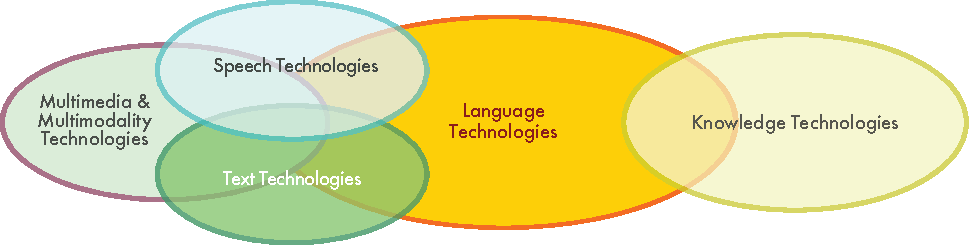
\includegraphics[width=\textwidth]{../_media/english/language_technologies}
  \caption{Language technology in context}
  \label{fig:ltincontext_en}
  \colorrule{grey3}{\textwidth}{1.5pt}
\end{figure*}

When we communicate, we combine language with other modes of communication and information media -- for example speaking can involve gestures and facial expressions. Digital texts link to pictures and sounds. Movies may contain language in spoken and written form. In other words, speech and text technologies overlap and interact with other multimodal communication and multimedia technologies.

In this section, we will discuss the main application areas of language technology, i.\,e., language checking, web search, speech interaction, and machine translation. These applications and basic technologies include 

\begin{itemize}
\item spelling correction
\item authoring support
\item computer-assisted language learning
\item information retrieval 
\item information extraction
\item text summarisation
\item question answering
\item speech recognition 
\item speech synthesis 
\end{itemize}

Language technology is an established area of research with an extensive set of introductory literature. The interested reader is referred to the following references:  \cite{carstensen-etal1, jurafsky-martin01, manning-schuetze1, lt-world1, lt-survey1}. 

Before discussing the above application areas, we will briefly describe the architecture of a typical LT system.

\subsection{Application Architectures}

Software applications for language processing typically consist of several components that mirror different aspects of language. While such applications tend to be very complex, figure~\ref{fig:textprocessingarch_en} shows a highly simplified architecture of a typical text processing system. The first three modules handle the structure and meaning of the text input:

\begin{enumerate}
\item Pre-processing: cleans the data, analyses or removes format-ting, detects the input languages, replaces contractions (e.g. ``le’d thoil'' with ``le do thoil''), and so on.
\item Grammatical analysis: finds the verb, its subject and objects, modifiers and other sentence constituents; detects the sentence structure.
\item Semantic analysis: performs disambiguation (i.\,e., computes the appropriate meaning of words in a given context); resolves anaphora (i.\,e., which pronouns refer to which nouns in the sentence); represents the meaning of the sentence in a machine-readable way.
\end{enumerate}

After analysing the text, task-specific modules can perform other operations, such as automatic summarisation and database look-ups.

In the remainder of this section, we firstly introduce the core application areas for language technology, and follow this with a brief overview of the state of LT research and education today, and a description of past and present research programmes. Finally, we present an expert estimate of core LT tools and resources for Irish in terms of various dimensions such as availability, maturity and quality. The general situation of LT for the Irish language is summarised in a matrix (figure~\ref{fig:lrlttable_en}). Tools and resources that are boldfaced in the text can also be found in figure~\ref{fig:lrlttable_en} (p.~\pageref{fig:lrlttable_en}) at the end of this chapter. LT support for Irish is also compared to other languages that are part of this series.

\begin{figure*}[htb]
  \colorrule{grey3}{\textwidth}{1.5pt}
  \center
  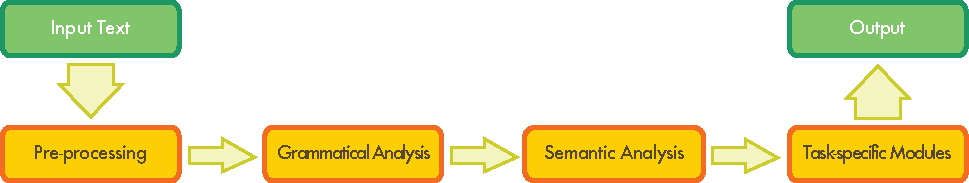
\includegraphics[width=\textwidth]{../_media/english/text_processing_app_architecture}
  \caption{A typical text processing architecture}
  \label{fig:textprocessingarch_en}
  \colorrule{grey3}{\textwidth}{1.5pt}
\end{figure*}

\subsection{Core Application Areas}

In this section, we focus on the most important LT tools and resources, and provide an overview of LT activities in Ireland. 

\subsubsection{Language Checking}

Anyone who has used a word processor such as Microsoft Word knows that it has a spell checker that highlights spelling mistakes and proposes corrections. The first spelling correction programs compared a list of extracted words against a dictionary of correctly spelled words. Today these programs are far more sophisticated. Using language-dependent algorithms for \textbf{grammatical analysis}, they detect errors related to morphology (e.\,g., plural formation) as well as syntax-related errors, such as a missing verb or a conflict of verb-subject agreement (e.\,g., \textit{she *write a letter}). However, most spell checkers will not find any errors in the following text \cite{zar1}:

\begin{quote}
  I have a spelling checker,\\
  It came with my PC.\\
  It plane lee marks four my revue\\
  Miss steaks aye can knot sea.
\end{quote}

Handling these kinds of errors usually requires an analysis of the context. This type of analysis either needs to draw on language-specific \textbf{grammars} laboriously coded into the software by experts, or on a statistical language model. In this case, a model calculates the probability of a particular word as it occurs in a specific position. A statistical language model can be automatically created by using a large amount of (correct) language data (called a \textbf{text corpus}). Most of these two approaches have been developed around data from English. Currently, neither approach can transfer easily to Irish because there are few language resources such as text corpora to train a statistical model and there is insufficient expertise to manu-ally encode linguistic knowledge in grammars.

\begin{figure*}[htb]
  \colorrule{grey3}{\textwidth}{1.5pt}
  \center
  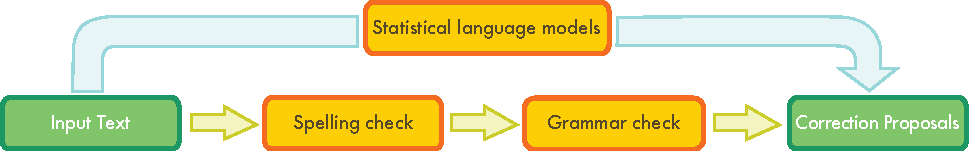
\includegraphics[width=\textwidth]{../_media/english/language_checking}
  \caption{Language checking (statistical; rule-based)}
  \label{fig:langcheckingaarch_en}
  \colorrule{grey3}{\textwidth}{1.5pt}
\end{figure*}

Language checking is not limited to word processors; it is also used in ``authoring support systems'', i.\,e., software environments in which manuals and other types of technical documentation for complex IT, healthcare, engineering and other products, are written. To offset customer complaints about incorrect use and damage claims resulting from poorly understood instructions, companies are increasingly focusing on the quality of technical documentation while targeting the international market (via translation or localisation) at the same time. Advances in natural language processing have led to the development of authoring support software, which helps the writer of technical documentation to use vocabulary and sentence structures that are consistent with industry rules and (corporate) terminology restrictions.

\boxtext{Language checking is not limited to word processors, but also applies to authoring systems.}

Language checking tools are available for Irish in popular office suites such as Microsoft Office and Open Office. These tools check not just spelling but also many aspects of Irish grammar however, direct integration into existing products is not always possible. For example, only one language checker for Irish \cite{gramadoir} does more than spelling correction, and it is currently not easily integrated into either OpenOffice or Microsoft Word (though, at the time of writ-ing, this is work in progress). With respect to spelling correction, Microsoft's spell checker has not been updated in many years.  There is only one spell checker (GaelSpell http://borel.slu.edu/ispell/) which is consistently updated, open source, and available for Word/OOo/Firefox, etc

Besides spell checkers and authoring support, language checking is also important in the field of computer-assisted language learning. Language checking applications also automatically correct search engine queries, as found in Google's \textit{Did you mean\ldots} suggestions.

\subsubsection{Web Search}

\begin{figure*}[htb]
  \colorrule{grey3}{\textwidth}{1.5pt}
  \center
  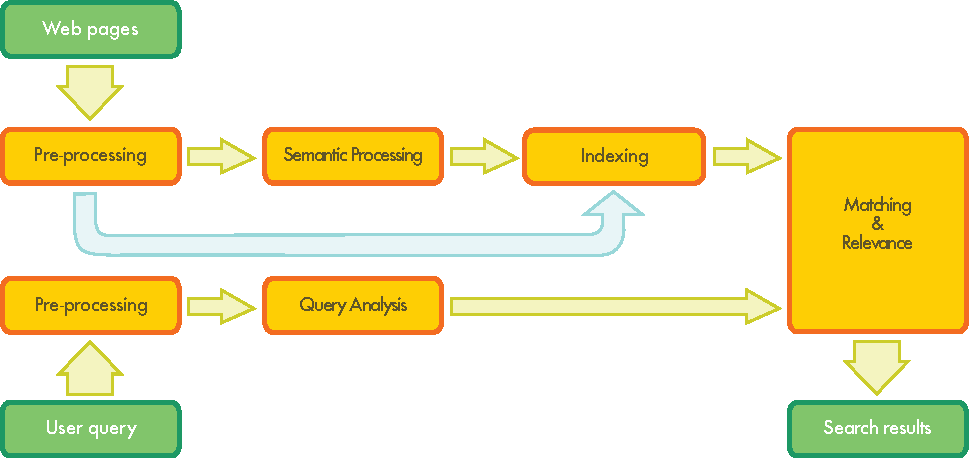
\includegraphics[width=\textwidth]{../_media/english/web_search_architecture}
  \caption{Web search architecture}
  \label{fig:websearcharch_en}
  \colorrule{grey3}{\textwidth}{1.5pt}
 \end{figure*}

Searching the Web, intranets or digital libraries is probably the most widely used yet largely underdeveloped language technology application today. The Google search engine, which started in 1998, now handles about 80\% of all search queries and over 90\% of all search queries from internet users in Ireland \cite{googlemarketshare}. As of the time of writing there is not yet an official Irish equivalent of the verb ``to google'' as there is in for example, German. But certainly in the vernacular where, English loan words first creep into the language the term ``gúgláil'' \cite{kilgarriff2010} is used. The Google search interface and re-sults page display has not significantly changed since the first version. Yet in the current version, Google offers spelling correction for misspelled words (but not for Irish) and has now incorporated basic semantic search capabilities that can improve search accuracy by analysing the meaning of terms in a search query context \cite{googlesemsearch}.  The Google success story shows that a large volume of available data and efficient indexing techniques can deliver satisfactory results for a statistically-based approach. 

For more sophisticated information requests, it is essential to integrate deeper linguistic knowledge to facilitate text interpretation. Experiments using \textbf{lexical resources} such as machine-readable thesauri or ontological language resources (e.g., WordNet for English or Líonra Séimeantach na Gaeilge for Irish) have demonstrated improvements in finding pages using synonyms of the original search terms, such as \textit{fuinnimh adamach} [atomic energy], \textit{cumhacht núicléach} [nuclear energy], or even more loosely related terms. 

\boxtext{The next generation of search engines will have to include much more sophisticated language technology.}

The next generation of search engines will have to include much more sophisticated language technology, especially to deal with search queries consisting of a question or other sentence type rather than a list of keywords. For the query, \textit{Give me a list of all companies that were taken over by other companies in the last five years}, a syntactic as well as \textbf{semantic analysis} is required. The system also needs to provide an index to quickly retrieve relevant documents. A satisfactory answer will require syntactic parsing to analyse the grammatical structure of the sentence and determine that the user wants companies that have been acquired, rather than companies that have acquired other companies. For the expression \textit{last five years}, the system needs to determine the relevant range of years, taking into account the present year. The query then needs to be matched against a huge amount of unstructured data to find the pieces of information that are relevant to the user's request. This process is called information retrieval, and involves searching and ranking relevant documents. To generate a list of companies, the system also needs to recognise a particular string of words in a document represents a company name, using a process called named entity recognition.

A more demanding challenge is matching a query in one language with documents in another language. Cross-lingual information retrieval involves automatically translating the query into all possible source languages and then translating the results back into the user's target language.

Now that data is increasingly found in non-textual formats, there is a need for services that deliver multimedia information retrieval by searching images, audio files and video data. In the case of audio and video files, a speech recognition module must convert the speech content into text (or into a phonetic representation) that can then be matched against a user query.

In Ireland, a number of small providers like Maithú Teoranta and various academic groups provide component language technologies for lexical analysis and similar tasks which could be employed in web search. A search engine for Irish, http://aimsigh.com, which is tailored to the language (stemmed searches etc.) has existed since ca. 2005-2006 but the owner says the project is currently defunct as it was/is largely unused so he feels it is ``not worth investing in research/development of such things if it's been proven Irish speakers don't really care to use them - they're satisfied with Google.'' Therefore, there is currently no large scale Irish language search engine project/product aside from Google’s Irish interface which while localised, is not optimised or tailored to work in the language.

\subsubsection{Speech Interaction}

Speech interaction is one of many application areas that depend on speech technology, i.\,e., technologies for processing spoken language. Speech interaction technology is used to create interfaces that enable users to interact in spoken language instead of using a graphical display, keyboard and mouse.  Today, these voice user interfaces (VUI) are used for partially or fully automated telephone services provided by companies to customers, employees or partners. Business domains that rely heavily on VUIs include banking, supply chain, public transportation, and telecommunications. Other uses of speech interaction technology include interfaces to car navigation systems and the use of spoken language as an alternative to the graphical or touchscreen interfaces in smartphones.

\begin{figure*}[htb]
  \colorrule{grey3}{\textwidth}{1.5pt}
  \center
  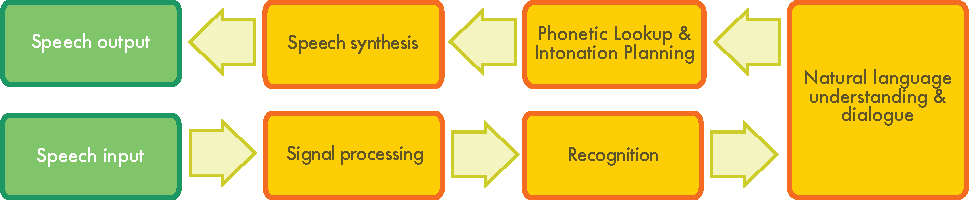
\includegraphics[width=\textwidth]{../_media/english/simple_speech-based_dialogue_architecture}
  \caption{Speech-based dialogue system}
  \label{fig:dialoguearch_en}
  \colorrule{grey3}{\textwidth}{1.5pt}
\end{figure*}

Speech interaction technology comprises four technologies: 

\begin{enumerate}
\item Automatic \textbf{speech recognition} (ASR) determines which words are actually spoken in a given sequence of sounds uttered by a user.  
\item Natural language understanding analyses the syntactic structure of a user's utterance and interprets it according to the system in question.
\item Dialogue management determines which action to take given the user input and system functionality.   
\item \textbf{Speech synthesis} (text-to-speech or TTS) transforms the system's reply into sounds for the user.
\end{enumerate}

One of the major challenges of ASR systems is to accurately recognise the words a user utters. This means restricting the range of possible user utterances to a limited set of keywords, or manually creating language models that cover a large range of natural language utterances. Using machine learning techniques, language models can also be generated automatically from \textbf{speech corpora}, i.\,e., large collections of speech audio files and text transcriptions. Restricting utterances usually forces people to use the voice user interface in a rigid way and can damage user acceptance; but the creation, tuning and maintenance of rich language models will significantly increase costs. VUIs that employ language models and initially allow a user to express their intent more flexibly -- prompted by a \textit{How may I help you?} greeting -- tend to be automated and are better accepted by users.

\boxtext{Speech interaction is the basis for interfaces that allow a user to interact with spoken language.}

Companies tend to use utterances pre-recorded by professional speakers for generating the output of the voice user interface. For static utterances where the wording does not depend on particular contexts of use or personal user data, this can deliver a rich user experience. But more dynamic content in an utterance may suffer from unnatural intonation because different parts of audio files have simply been strung together. Through optimisation, today's TTS systems are getting better at producing natural-sounding dynamic utterances.

Interfaces in speech interaction have been considerably standardised during the last decade in terms of their various technological components. There has also been strong market consolidation in speech recognition and speech synthesis. The national markets in the G20 countries (economically resilient countries with high populations) have been dominated by just five global players, with Nuance (USA) and Loquendo (Italy) being the most prominent players in Europe. In 2011, Nuance announced the acquisition of Loquendo, which represents a further step in market consolidation.

Synthesisers and recognisers exist for Irish through a number of academic projects. However, at the time of writing we are unaware of any commercial applications aside from some learning tools (which most likely use pre recorded segments instead of full synthesis) which employ speech technologies for Irish.

Looking ahead, there will be significant changes, due to the spread of smartphones as a new platform for managing customer relationships, in addition to fixed telephones, the Internet and e-mail. This will also affect how speech interaction technology is used. In the long term, there will be fewer telephone-based VUIs, and spoken language apps will play a far more central role as a user-friendly input for smartphones. This will be largely driven by stepwise improvements in the accuracy of speaker-independent speech recognition via the speech dictation services already offered as centralised services to smartphone users.

\subsubsection{Machine Translation}

The idea of using digital computers to translate natural languages can be traced back to 1946 and was followed by substantial funding for research during the 1950s and again in the 1980s. 
Yet machine translation (MT) still cannot deliver on its initial promise of providing across-the-board automated translation.  

\boxtext{At its basic level, Machine Translation simply substitutes words in one natural language with words in another language.}

The most basic approach to machine translation is the automatic replacement of the words in a text written in one natural language with the equivalent words of another language. This can be useful in subject domains that have a very restricted, formulaic language such as weather reports. However, in order to produce a good translation of less restricted texts, larger text units (phrases, sentences, or even whole passages) need to be matched to their closest counterparts in the target language. The major difficulty is that human language is ambiguous. Ambiguity creates challenges on multiple levels, such as word sense disambiguation at the lexical level (a \textit{jaguar} is a brand of car or an animal) or the assignment of case on the syntactic level.

One way to build an MT system is to use linguistic rules. For translations between closely related languages, a translation using direct substitution may be feasible in cases such as the above example. However, rule-based (or linguistic knowledge-driven) systems often analyse the input text and create an intermediary symbolic representation from which the target language text can be generated. The success of these methods is highly dependent on the availability of extensive lexicons with morphological, syntactic, and semantic information, and large sets of grammar rules carefully designed by skilled linguists. This is a very long and therefore costly process.

\begin{figure*}[htb]
  \colorrule{grey3}{\textwidth}{1.5pt}
  \center
  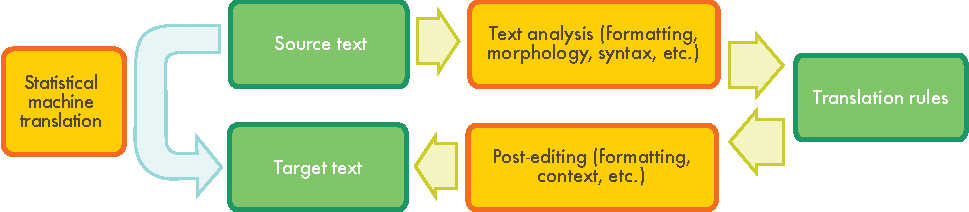
\includegraphics[width=\textwidth]{../_media/english/machine_translation}
  \caption{Machine translation (left: statistical; right: rule-based)}
  \label{fig:mtarch_en}
  \colorrule{grey3}{\textwidth}{1.5pt}
\end{figure*}

In the late 1980s when computational power increased and became cheaper, interest in statistical models for machine translation began to grow. Statistical models are derived from analysing bilingual text corpora, \textbf{parallel corpora}, such as the Europarl parallel corpus, which contains the proceedings of the European Parliament in 21 European languages. Given enough data, statistical MT works well enough to derive an approximate meaning of a foreign language text by processing parallel versions and finding plausible patterns of words. Unlike knowledge-driven systems, however, statistical (or data-driven) MT systems often generate ungrammatical output. Data-driven MT is advantageous because less human effort is required, and it can also cover special particularities of the language (e.\,g., idiomatic expressions) that are often ignored in knowledge-driven systems. 

\boxtext{Machine Translation is particularly challenging for the Irish language due to a lack of resources.}

The strengths and weaknesses of knowledge-driven and data-driven machine translation tend to be complementary, so that nowadays researchers focus on hybrid approaches that combine both methodologies. One such approach uses both knowledge-driven and data-driven systems, together with a selection module that decides on the best output for each sentence. However, results for sentences longer than, say, 12 words, will often be far from perfect. A more effective solution is to combine the best parts of each sentence from multiple outputs; this can be fairly complex, as corresponding parts of multiple alternatives are not always obvious and need to be aligned. 

There is still a huge potential for improving the quality of MT systems. The challenges involve adapting language resources to a given subject domain or user area, and integrating the technology into workflows that already have term bases and translation memories. Another problem is that most of the current systems are English-centred and only support a few languages from and into Irish. This leads to friction in the translation workflow and forces MT users to learn different lexicon coding tools for different systems.

Evaluation campaigns help to compare the quality of MT systems, their approaches and the status of the systems for different language pairs. Figure~\ref{fig:euromatrix_de} (p.~\pageref{fig:euromatrix_de}), which was prepared during the Euromatrix+ project, shows the pair-wise performances obtained for 22 of the 23 official EU languages (Irish was not included in the comparison due to a lack of available tools). The results are ranked according to a BLEU score, which indicates higher scores for better translations \cite{bleu1}. A human translator would normally achieve a score of around 80 points. The best results (in green and blue) were achieved by languages that benefit from a considerable research effort in coordinated programmes and the existence of many parallel corpora (e.\,g., English, French, Dutch, Spanish and German). The languages with poorer results are shown in red. These languages either lack such development efforts or are structurally very different from other languages (e.\,g., Hungarian, Maltese and Finnish).

\subsection{Other Application Areas}

Building language technology applications involves a range of subtasks that do not always surface at the level of interaction with the user, but they provide significant service functionalities ``behind the scenes'' of the system in question. They all form important research issues that have now evolved into individual sub-disciplines of computational linguistics. Question answering, for example, is an active area of research for which annotated corpora have been built and scientific competitions have been initiated. The concept of question answering goes beyond keyword-based searches (in which the search engine responds by delivering a collection of potentially relevant documents) and enables users to ask a concrete question to which the system provides a single answer. For example:

\begin{itemize}
\item[] \textit{Question: How old was Neil Armstrong when he stepped on the moon?}
\item[] \textit{Answer: 38.}
\end{itemize}

While question answering is obviously related to the core area of web search, it is nowadays an umbrella term for such research issues as which different types of questions exist, and how they should be handled; how a set of documents that potentially contain the answer can be analysed and compared (do they provide conflicting answers?); and how specific information (the answer) can be reliably extracted from a document without ignoring the context. Question answering is in turn related to information extraction (IE), an area that was extremely popular and influential when computational linguistics took a statistical turn in the early 1990s. IE aims to identify specific pieces of information in specific classes of documents, such as the key players in company takeovers as reported in newspaper stories. Another common scenario that has been studied is reports on terrorist incidents. The task here consists of mapping appropriate parts of the text to a template that specifies the perpetrator, target, time, location and results of the incident. Domain-specific template-filling is the central characteristic of IE, which makes it another example of a ``behind the scenes'' technology that forms a well-demarcated research area, which in practice needs to be embedded into a suitable application environment. 

\boxtext{Language technology applications often provide significant service functionalities behind the scenes of larger software systems.}

Text summarisation and \textbf{text generation} are two borderline areas that can act either as standalone applications or play a supporting role. Summarisation attempts to give the essentials of a long text in a short form, and is one of the features available in Microsoft Word. It mostly uses a statistical approach to identify the ``important'' words in a text (i.\,e., words that occur very frequently in the text in question but less frequently in general language use) and determine which sentences contain the most of these ``important'' words. These sentences are then extracted and put together to create the summary. In this very common commercial scenario, summarisation is simply a form of sentence extraction, and the text is reduced to a subset of its sentences. An alternative approach, for which some research has been carried out, is to generate brand new sentences that do not exist in the source text. 

\boxtext{For the Irish language, research in most text technologies is much less developed than for most European languages.}

This requires a deeper understanding of the text, which means that so far this approach is far less robust. On the whole, a text generator is rarely used as a stand-alone application but is embedded into a larger software environment, such as a clinical information system that collects, stores and processes patient data. Creating reports is just one of many applications for text summarisation. 

For the Irish language, research in these text technologies is much less developed than for other European languages. Question answering, information extraction, and summarization have been the focus of numerous open competitions in the USA since the 1990s, primarily organised by the government-sponsored organisations DARPA and NIST. These competitions have significantly improved the start-of-the-art, but their focus has mostly been on the English language. As a result, the annotated corpora and other special re-sources needed to perform these tasks in other languages are not as well developed. While some exist for better resourced European languages such as German, there are virtually none of the necessary tools and resources available for Irish.

\subsection{Language Technology Industry and Programmes}

User and provider industries exist for Irish LT but largely focused around localization and translation services as a result of the Languages Act and becoming an official EU language. There is also a growing market in education as teaching practice embraces new technologies. Likewise, among the younger generations there is an emerging trend towards for the need for improved LT support for Irish.

The language industry is a significant employer in Ireland. Growing from approximately 4-5k jobs in the mid 90’s to over 12k at the turn of the century, currently this has levelled off somewhat with estimates of around 14-16k direct jobs in the localisation and translation industry in Ireland.

There are several excellent centres for linguistics and language technology research and industrial development, for example Microsoft, IBM, and Symantec all have a presence in Ireland working to some degree with various aspects of LT. But very little work is done on Irish language data by these players.

A number of SME's have appeared producing for example, mobile dictionary applications for Irish. As the mobile and social network markets grow the opportunity for businesses providing such language technologies for Irish will also receive a boost.

Despite the strong employment figures for the language industry in Ireland and growing opportunities in the domestic market for the national language, much of the work of LT is ``hidden'' from the end user/consumer. This is, many would argue as it should be as LT is very much an enabling technology providing components to simplify, improve or revolutionise how we interact with other products and services. For example, we do not think about what goes on in the components of our car engines, we are just happy that they work well. However, this situation creates its own difficulty for us in the LT community in that it becomes difficult to communicate to many groups the benefits and demands for language technologies. This in turn leads to a situation where many people working in related fields find it hard to see the benefit of using LT in their field.

A market for Irish language technologies is really only beginning to emerge now. In part, this is emerging from the already mature existing language technology/service providers and users, but also from demand being generated by the educated ``urban'' Irish speakers. This is being facilitated by the huge growth in ICT in Ireland and recent improvements in infrastructure to support this. It is also due, in no small part, to the growth of online activities, specifically social networking and learning activities, in younger generations who are exposed to the language almost daily and are usually early adopters of such technologies in their lifestyles.

\subsection{Language Technology Research and Education in Ireland}

Ireland is home to a number of leading research institutions in the field of computational linguistics, and has a National Centre for Language Technology located at Dublin City University alongside the Centre for Next Generation Localisation, which works on using computational linguistics to bring added value to globalisation, localisation and information access. Both of these centres are well established and have strong links with industrial R\&D both locally and abroad, as well as strong ties with other European centres of excellence in the field. The machine translation research team based at the CNGL is among the largest and most successful in the world. With such expertise available in Irish institutions it stands out that the situation for language technologies for Irish is not better. 

However, there is currently only 1 undergraduate degree in computational linguistics available at Irish universities. This single degree course only admits 25 students per year, of which 5 places are given an emphasis on Irish. With such a small pool of appropriately skilled graduates entering the workforce through the Irish education system, it is not surprising that the work done at Irish research centres is more significant for other languages than it is for Irish.

The computational linguistics and language technology community in Ireland is, relatively speaking, quite a small but active community. There is a lot of interaction and cooperation between institutes and industry partners in order to keep the field alive in Ireland. However, outside of events for the centres mentioned and some university events there is no real conference or community event for Irish LT.

\subsection{Availability of Tools and Resources}

Figure~\ref{fig:lrlttable_en} provides a rating for language technology support for the Irish language. This rating of existing tools and resources was generated by leading experts in the field who provided estimates based on a scale from 0 (very low) to 6 (very high) using seven criteria.

\begin{figure*}[htb]
\centering
%\begin{tabular}{>{\columncolor{orange1}}p{.33\linewidth}ccccccc} % ORIGINAL
\begin{tabular}{>{\columncolor{orange1}}p{.33\linewidth}@{\hspace*{6mm}}c@{\hspace*{6mm}}c@{\hspace*{6mm}}c@{\hspace*{6mm}}c@{\hspace*{6mm}}c@{\hspace*{6mm}}c@{\hspace*{6mm}}c}
\rowcolor{orange1}
 \cellcolor{white}&\begin{sideways}\makecell[l]{Quantity}\end{sideways}
&\begin{sideways}\makecell[l]{\makecell[l]{Availability} }\end{sideways} &\begin{sideways}\makecell[l]{Quality}\end{sideways}
&\begin{sideways}\makecell[l]{Coverage}\end{sideways} &\begin{sideways}\makecell[l]{Maturity}\end{sideways} &\begin{sideways}\makecell[l]{Sustainability}\end{sideways} &\begin{sideways}\makecell[l]{Adaptability}\end{sideways} \\ \addlinespace
\multicolumn{8}{>{\columncolor{orange2}}l}{Language Technology: Tools, Technologies and Applications} \\ \addlinespace
Speech Recognition	&5&1&3&2&4&3&3 \\ \addlinespace
Speech Synthesis &5&3&3&2&4&3&3\\ \addlinespace
Grammatical analysis &4&2.5&2&2&4&2.5&2.5\\ \addlinespace
Semantic analysis &2&2&0&0&2&2&1\\ \addlinespace
Text generation &2&1&2&2&2&1&2\\ \addlinespace
Machine translation &5&3&1&1&4&1&2\\ \addlinespace
\multicolumn{8}{>{\columncolor{orange2}}l}{Language Resources: Resources, Data and Knowledge Bases} \\ \addlinespace
Text corpora &3&2&1&1&4&4&2.5\\ \addlinespace
Speech corpora &3&1&2&1&3&3&2\\ \addlinespace
Parallel corpora &2&1&2&1&2&2&1\\ \addlinespace
Lexical resources &3&2.5&2&2&4&4&2.5\\ \addlinespace
Grammars &3&2&1&1&3&2&1\\
\end{tabular}
\caption{State of language technology support for Irish}
\label{fig:lrlttable_en}
\end{figure*}

The key results for Irish language technology can be summed up as follows:

\begin{itemize}
\item There are precious few tools and resources available for Irish. 
\item Quality, quantity and availability are issues for Irish language technology. Where tools exist they are usually good, but they are usually few or may not be widely available. Conversely, where they are widely available the quality tends to be lower or they are for a particular domain or task. 
\item The tools that do exist while of good quality often exist in isolation. There is often only one system for a particular task which can limit options.
\item Many of the resources are not readily available or easily adapted to new tasks.
\item Speech processing research seems to be quite well advanced compared to other areas such as text processing and language modelling despite the fact that basic text tools for Irish are available in several commercial applications. This would indicate that there is demand for  such basic tools even of lesser quality. 
\item Despite the availability of good resources for eg. speech processing this area is hampered by poor availability, coverage and unsustainable data.
\item There is a huge gap in data for use with language tools.
\item There is a lack of core component technologies for Irish which would enable more the more sophisticated language processing needed to build complex applications.
\item Good quality basic word analysis tooling and resources exist but there are not many of these tools and they lack adaptability
\end{itemize}

The results show that there is limited technological support for Irish and that the basic linguistic resources to support the development of core technologies are largely absent. It is clear that when investments in such tools and resources are made that quality tools and resources can be created. But it seems that a lack of direction in the development of such tools and resources has stilted progress.

\subsection{Cross-language comparison}
The current state of LT support varies considerably from one language community to another. In order to compare the situation between languages, this section will present an evaluation based on two sample application areas (machine translation and speech processing) and one underlying technology (text analysis), as well as basic resources needed for building LT applications. The languages were categorised using the following five-point scale: 

\begin{enumerate}
\item Excellent support
\item Good support
\item Moderate support
\item Fragmentary support
\item Weak or no support
\end{enumerate}

Language Technology support was measured according to the following criteria:

\textbf{Speech Processing:} Quality of existing speech recognition technologies, quality of existing speech synthesis technologies, coverage of domains, number and size of existing speech corpora, amount and variety of available speech-based applications.

\textbf{Machine Translation:} Quality of existing MT technologies, number of language pairs covered, coverage of linguistic phenomena and domains, quality and size of existing parallel corpora, amount and variety of available MT applications.

\textbf{Text Analysis:} Quality and coverage of existing text analysis technologies (morphology, syntax, semantics), coverage of linguistic phenomena and domains, amount and variety of available applications, quality and size of existing (annotated) text corpora, quality and coverage of existing lexical resources (e.\,g., WordNet) and grammars.

\textbf{Resources:} Quality and size of existing text corpora, speech corpora and parallel corpora, quality and coverage of existing lexical resources and grammars.

Figures~\ref{fig:speech_cluster_en} to~\ref{fig:resources_cluster_en} show that Irish is not very well equipped with language technologies or language resources. The current research and development efforts, which have provided some resources for the Irish language, while providing a much needed step in the right direction are still lagging behind other languages and falling well behind English.

However, the clustering shows that Irish is not alone in this situation. Many other European languages are facing this same difficulty. A key differentiating factor, though, is that most of these other languages far outnumber Irish in the number of speakers and also they are not competing with a much better resourced language like English nor are they minority languages in the regions where they are spoken.

Looking at the tables in this light we can see that without making some drastic changes very much Irish is at risk of being left behind other languages as Language Technology advances are made. This is a serious situation for Ireland both politically and socially. Fortunately, Ireland still has a strong indigenous language services industry and is home to several world class LT research centres. By applying this expertise to the problems facing the Irish language Ireland could rapidly equip the Irish language to take a massive step forward into the information age. The resultant social and economic benefits through employment, R\&D path to market and increased enablement for Irish language speakers has the potential to make Ireland a leading light in LT for under-resourced languages while at the same time addressing many stumbling blocks for uptake of the Irish language. Such an effort is entirely possible in Ireland given the indigenous LT expertise, however greater engagement with LT from the Irish language community as well as a concerted national approach encompassing research, industry and language policy is needed to realise this goal.
\begin{figure*}[tb]
  \small
  \centering
  \begin{tabular}
  { % defines color for each column.
  >{\columncolor{corange5}}p{.13\linewidth}@{\hspace{.040\linewidth}}
  >{\columncolor{corange4}}p{.13\linewidth}@{\hspace{.040\linewidth}}
  >{\columncolor{corange3}}p{.13\linewidth}@{\hspace{.040\linewidth}}
  >{\columncolor{corange2}}p{.13\linewidth}@{\hspace{.040\linewidth}}
  >{\columncolor{corange1}}p{.13\linewidth} 
  }
  \multicolumn{1}{>{\columncolor{white}}c@{\hspace{.040\linewidth}}}{\textbf{Excellent}} & 
  \multicolumn{1}{@{}>{\columncolor{white}}c@{\hspace{.040\linewidth}}}{\textbf{Good}} &
  \multicolumn{1}{@{}>{\columncolor{white}}c@{\hspace{.040\linewidth}}}{\textbf{Moderate}} &
  \multicolumn{1}{@{}>{\columncolor{white}}c@{\hspace{.040\linewidth}}}{\textbf{Fragmentary}} &
  \multicolumn{1}{@{}>{\columncolor{white}}c}{\textbf{Weak/no}} \\ 
  \multicolumn{1}{>{\columncolor{white}}c@{\hspace{.040\linewidth}}}{\textbf{support}} & 
  \multicolumn{1}{@{}>{\columncolor{white}}c@{\hspace{.040\linewidth}}}{\textbf{support}} &
  \multicolumn{1}{@{}>{\columncolor{white}}c@{\hspace{.040\linewidth}}}{\textbf{support}} &
  \multicolumn{1}{@{}>{\columncolor{white}}c@{\hspace{.040\linewidth}}}{\textbf{support}} &
  \multicolumn{1}{@{}>{\columncolor{white}}c}{\textbf{support}} \\ \addlinespace
  
& \vspace*{0.5mm}English
& \vspace*{0.5mm}
Czech \newline 
Dutch \newline 
Finnish \newline 
French \newline 
German \newline   
Italian \newline  
Portuguese \newline 
Spanish \newline
& \vspace*{0.5mm}Basque \newline 
Bulgarian \newline 
Catalan \newline 
Danish \newline 
Estonian \newline 
Galician\newline 
Greek \newline  
Hungarian  \newline
\textbf{Irish} \newline  
Norwegian \newline 
Polish \newline 
Serbian \newline 
Slovak \newline 
Slovene \newline 
Swedish \newline
& \vspace*{0.5mm}
Croatian \newline 
Icelandic \newline  
Latvian \newline 
Lithuanian \newline 
Maltese \newline 
Romanian\\
\end{tabular}
\caption{Speech processing: state of language technology support for 30 European languages}
\label{fig:speech_cluster_en}
\end{figure*}

\begin{figure*}[tb]
  \small
  \centering
  \begin{tabular}
  { % defines color for each column.
  >{\columncolor{corange5}}p{.13\linewidth}@{\hspace{.040\linewidth}}
  >{\columncolor{corange4}}p{.13\linewidth}@{\hspace{.040\linewidth}}
  >{\columncolor{corange3}}p{.13\linewidth}@{\hspace{.040\linewidth}}
  >{\columncolor{corange2}}p{.13\linewidth}@{\hspace{.040\linewidth}}
  >{\columncolor{corange1}}p{.13\linewidth} 
  }
  \multicolumn{1}{>{\columncolor{white}}c@{\hspace{.040\linewidth}}}{\textbf{Excellent}} & 
  \multicolumn{1}{@{}>{\columncolor{white}}c@{\hspace{.040\linewidth}}}{\textbf{Good}} &
  \multicolumn{1}{@{}>{\columncolor{white}}c@{\hspace{.040\linewidth}}}{\textbf{Moderate}} &
  \multicolumn{1}{@{}>{\columncolor{white}}c@{\hspace{.040\linewidth}}}{\textbf{Fragmentary}} &
  \multicolumn{1}{@{}>{\columncolor{white}}c}{\textbf{Weak/no}} \\ 
  \multicolumn{1}{>{\columncolor{white}}c@{\hspace{.040\linewidth}}}{\textbf{support}} & 
  \multicolumn{1}{@{}>{\columncolor{white}}c@{\hspace{.040\linewidth}}}{\textbf{support}} &
  \multicolumn{1}{@{}>{\columncolor{white}}c@{\hspace{.040\linewidth}}}{\textbf{support}} &
  \multicolumn{1}{@{}>{\columncolor{white}}c@{\hspace{.040\linewidth}}}{\textbf{support}} &
  \multicolumn{1}{@{}>{\columncolor{white}}c}{\textbf{support}} \\ \addlinespace
  
& \vspace*{0.5mm} English 
& \vspace*{0.5mm} 
French \newline 
Spanish
& \vspace*{0.5mm}
Catalan \newline 
Dutch \newline 
German \newline 
Hungarian \newline
Italian \newline 
Polish \newline 
Romanian \newline 
& \vspace*{0.5mm}Basque \newline 
Bulgarian \newline 
Croatian \newline 
Czech \newline
Danish \newline 
Estonian \newline 
Finnish \newline 
Galician \newline 
Greek \newline 
Icelandic \newline 
\textbf{Irish} \newline 
Latvian \newline 
Lithuanian \newline 
Maltese \newline 
Norwegian \newline 
Portuguese \newline 
Serbian \newline 
Slovak \newline 
Slovene \newline 
Swedish \newline 
\end{tabular}
\caption{Machine translation: state of language technology support for 30 European languages}
\label{fig:mt_cluster_en}
\end{figure*}

\begin{figure*}[tb]
  \small
  \centering
  \begin{tabular}
  { % defines color for each column.
  >{\columncolor{corange5}}p{.13\linewidth}@{\hspace{.040\linewidth}}
  >{\columncolor{corange4}}p{.13\linewidth}@{\hspace{.040\linewidth}}
  >{\columncolor{corange3}}p{.13\linewidth}@{\hspace{.040\linewidth}}
  >{\columncolor{corange2}}p{.13\linewidth}@{\hspace{.040\linewidth}}
  >{\columncolor{corange1}}p{.13\linewidth} 
  }
  \multicolumn{1}{>{\columncolor{white}}c@{\hspace{.040\linewidth}}}{\textbf{Excellent}} & 
  \multicolumn{1}{@{}>{\columncolor{white}}c@{\hspace{.040\linewidth}}}{\textbf{Good}} &
  \multicolumn{1}{@{}>{\columncolor{white}}c@{\hspace{.040\linewidth}}}{\textbf{Moderate}} &
  \multicolumn{1}{@{}>{\columncolor{white}}c@{\hspace{.040\linewidth}}}{\textbf{Fragmentary}} &
  \multicolumn{1}{@{}>{\columncolor{white}}c}{\textbf{Weak/no}} \\ 
  \multicolumn{1}{>{\columncolor{white}}c@{\hspace{.040\linewidth}}}{\textbf{support}} & 
  \multicolumn{1}{@{}>{\columncolor{white}}c@{\hspace{.040\linewidth}}}{\textbf{support}} &
  \multicolumn{1}{@{}>{\columncolor{white}}c@{\hspace{.040\linewidth}}}{\textbf{support}} &
  \multicolumn{1}{@{}>{\columncolor{white}}c@{\hspace{.040\linewidth}}}{\textbf{support}} &
  \multicolumn{1}{@{}>{\columncolor{white}}c}{\textbf{support}} \\ \addlinespace

& \vspace*{0.5mm}English
& \vspace*{0.5mm}
  Dutch \newline 
  French \newline 
  German \newline 
  Italian \newline 
  Spanish
& \vspace*{0.5mm}Basque \newline 
  Bulgarian \newline 
  Catalan \newline 
  Czech \newline 
  Danish \newline 
  Finnish \newline 
  Galician \newline 
  Greek \newline 
  Hungarian \newline 
  Norwegian \newline 
  Polish \newline 
  Portuguese \newline 
  Romanian \newline 
  Slovak \newline 
  Slovene \newline 
  Swedish \newline 
& \vspace*{0.5mm}
  Croatian \newline 
  Estonian \newline 
  Icelandic \newline 
  \textbf{Irish} \newline 
  Latvian \newline 
  Lithuanian \newline 
  Maltese \newline 
  Serbian \\
  \end{tabular}
\caption{Text analysis: state of language technology support for 30 European languages}
\label{fig:text_cluster_en}
\end{figure*}

\begin{figure*}[tb]
  \small
  \centering
  \begin{tabular}
  { % defines color for each column.
  >{\columncolor{corange5}}p{.13\linewidth}@{\hspace{.040\linewidth}}
  >{\columncolor{corange4}}p{.13\linewidth}@{\hspace{.040\linewidth}}
  >{\columncolor{corange3}}p{.13\linewidth}@{\hspace{.040\linewidth}}
  >{\columncolor{corange2}}p{.13\linewidth}@{\hspace{.040\linewidth}}
  >{\columncolor{corange1}}p{.13\linewidth} 
  }
  \multicolumn{1}{>{\columncolor{white}}c@{\hspace{.040\linewidth}}}{\textbf{Excellent}} & 
  \multicolumn{1}{@{}>{\columncolor{white}}c@{\hspace{.040\linewidth}}}{\textbf{Good}} &
  \multicolumn{1}{@{}>{\columncolor{white}}c@{\hspace{.040\linewidth}}}{\textbf{Moderate}} &
  \multicolumn{1}{@{}>{\columncolor{white}}c@{\hspace{.040\linewidth}}}{\textbf{Fragmentary}} &
  \multicolumn{1}{@{}>{\columncolor{white}}c}{\textbf{Weak/no}} \\ 
  \multicolumn{1}{>{\columncolor{white}}c@{\hspace{.040\linewidth}}}{\textbf{support}} & 
  \multicolumn{1}{@{}>{\columncolor{white}}c@{\hspace{.040\linewidth}}}{\textbf{support}} &
  \multicolumn{1}{@{}>{\columncolor{white}}c@{\hspace{.040\linewidth}}}{\textbf{support}} &
  \multicolumn{1}{@{}>{\columncolor{white}}c@{\hspace{.040\linewidth}}}{\textbf{support}} &
  \multicolumn{1}{@{}>{\columncolor{white}}c}{\textbf{support}} \\ \addlinespace
    
& \vspace*{0.5mm}English
& \vspace*{0.5mm} 
    Czech \newline 
    Dutch \newline 
    French \newline 
    German \newline 
    Hungarian \newline
    Italian \newline
    Polish \newline
    Spanish \newline
    Swedish \newline 
& \vspace*{0.5mm} Basque\newline 
    Bulgarian\newline 
    Catalan \newline 
    Croatian \newline 
    Danish \newline 
    Estonian \newline 
    Finnish \newline 
    Galician \newline 
    Greek \newline 
    Norwegian \newline 
    Portuguese \newline 
    Romanian \newline 
    Serbian \newline 
    Slovak \newline 
    Slovene \newline
&  \vspace*{0.5mm}
    Icelandic \newline 
    \textbf{Irish} \newline 
    Latvian \newline 
    Lithuanian \newline 
    Maltese  \\
  \end{tabular}
  \caption{Speech and text resources: State of support for 30 European languages}  
  \label{fig:resources_cluster_en}
\end{figure*}




\subsection{Conclusions}

\emph{In this series of white papers, we have made an important effort by assessing the language technology support between 30 European languages, and by providing a high-level comparison across these languages. By identifying the gaps, needs and deficits, the European language technology community and its related stakeholders are now in a position to design a large scale research and development programme aimed at building a truly multilingual, technology-enabled communication across Europe.}

The results of this white paper series show that there is a dramatic difference in language technology support between the various European languages. While there are good quality software and resources available for some languages and application areas, others, usually smaller languages, have substantial gaps. Many languages lack basic technologies for text analysis and the essential resources. Others have basic tools and resources but the implementation of for example semantic methods is still far away. Therefore a large-scale effort is needed to attain the ambitious goal of providing high-quality language technology support for all European languages, for example through high quality machine translation. 

The EUROMAP Language Technologies \cite{euromap} project, 2003, has investigated the state-of-the-art of LT research and take-up in Europe, as well as the background for the present situation in each country. The report concludes that a visible presence for European LT activities should be established, for Europe as no other advanced economic area enjoys a similar cultural and linguistic diversity. The goal should be to have a set of robust, stable, multilingual HLT modules, capable of being embedded into emerging IST application environments. The study highlights Ireland’s strong position with respect to LT R\&D and notes that while Ireland is not leading the field in this area, it is performing in line with the EU average and, based on the metrics used, falls in a group of ``promising'' countries with respect to LT R\&D which need only to improve technology transfer to attain ``next generation'' standards.

%\begin{figure*}[htb]
%  \colorrule{grey3}{\textwidth}{1.5pt}
%  \center
%  \includegraphics[width=\textwidth]{./EuromapScorecard}
%  \caption{EUROMAP HLT Scorecard}
%  \label{fig:EuromapHLT_EN}
%  \colorrule{grey3}{\textwidth}{1.5pt}
%\end{figure*}
%NEED TO ADD DIAGRAM

The issue of technology transfer, as identified by EUROMAP is a key factor in securing a place for the Irish language in the modern information society. Various social, educational and political factors in Ireland have created a strong demand for ICT which caters for the growing demand for digital information in Irish. However, the lack of fluency in Irish among the general population and the lack of technology transfer from state of the art LT research in Ireland into applications which could support greater fluency and/or improve information access through Irish appear to be hindering taking the next step forward for Irish.

Ireland as a middle rank player in EU language technology, shares a language with the UK and the USA. This unique position in Western Europe means that as a nation it acts as a key bridge between the European and North American software industry. The country has chosen to focus its resources on building a powerful IT service industry rather than on developing a national language research base. As a result it hosts a significant concentration of language localisation expertise and research which has fuelled a strong industry around LT in the translation and localisation fields. Other leading research groups in core LT and next generation applications have sprung up in the light of this situation. However, they are largely focused towards supporting European and industrial goals. Hence, the state of the art language technologies developed in Ireland are slow in being applied to national interests and the Irish language itself.

The current situation where there is a clear and growing demand for technologies which both support and enable the Irish language represents a unique opportunity for LT research and development in Ireland. National and European initiatives and directives are creating a growing demand for translation and localisation of in-formation, documents and services into Irish. At the same time the demand for confident and competent speakers, translators and linguists in Irish is growing. This has created a demand, and an opportunity, for the creation of state of the art core LT resources for Irish, as well as the need to bridge the gap between research and the public at large by providing new and innovative tools which can support students of the language and those eager to partake in the information society through Irish. Leveraging existing LTs, developed in Ireland for other languages, for Irish and combining that with improved LT technology transfer to market can provide Ireland with a strong platform from which to stake its claim as a contender in the next generation of ICT industries, as well as providing a means to ensure a place for the Irish language in the in-formation society.

Our findings show that the only alternative is to make a substantial effort to create LT resources for Irish, and use them to drive for-ward research, innovation and development. The need for large amounts of data and the extreme complexity of language technology systems makes it vital to develop a new infrastructure and a more coherent research organization to spur greater sharing and cooperation.

There is also a lack of continuity in research and development funding. Short-term coordinated programmes tend to alternate with periods of sparse or zero funding. In addition, there is an overall lack of coordination with programmes in other EU countries and at the European Commission level.

We can therefore conclude that there is a desperate need for a large, coordinated initiative focused on overcoming the differences in language technology readiness for European languages as a whole.

META-NET’s long-term goal is to introduce high-quality language technology for all languages in order to achieve political and economic unity through cultural diversity. The technology will help tear down existing barriers and build bridges between Europe’s languages. This requires all stakeholders - in politics, research, business, and society - to unite their efforts for the future. A large coordinated effort focused on language technologies would help save the Irish language, together with other languages, and establish a genuine multilingual agenda for Europe and the world as a whole \cite{tcstar}. 


\end{multicols}

\clearpage

\ssection[About META-NET]{About META-NET}

\begin{multicols}{2}
META-NET is a Network of Excellence funded by the European Commission. The network currently consists of 54 members from 33 European countries \cite{rehm2011}. META-NET fosters the Multilingual Europe Technology Alliance (META), a growing community of language technology professionals and organisations in Europe. META-NET cooperates with other initiatives like the Common Language Resources and Technology Infrastructure (CLARIN), which is helping to establish digital humanities research in Europe. META-NET fosters the technological foundations for a truly multilingual European information society that:

\begin{itemize}
\item makes communication and cooperation possible across languages;
\item provides equal access to information and knowledge in any language;
\item offers advanced and affordable networked information technology to European citizens.
\end{itemize}

META-NET stimulates and promotes multilingual technologies for all European languages. The technologies enable automatic translation, content production, information processing and knowledge management for a wide variety of applications and subject domains. The network wants to improve current approaches, so better communication and cooperation across languages can take place. Europeans have an equal right to information and knowledge regardless of language.

META-NET launched on 1 February 2010 with the goal of advancing research in language technology (LT). The network supports a Europe that unites as a single digital market and information space. META-NET has conducted several activities that further its goals. META-VISION, META-SHARE and META-RESEARCH are the network's three lines of action.

\textbf{META-VISION} fosters a dynamic and influential stakeholder community that unites around a shared vision and a common strategic research agenda (SRA). The main focus of this activity is to build a coherent and cohesive LT community in Europe by bringing together representatives from highly fragmented and diverse groups of stakeholders. In the first year of META-NET, presentations at the FLaReNet Forum (Spain), Language Technology Days (Luxembourg), JIAMCATT 2010 (Luxembourg), LREC 2010 (Malta), EAMT 2010 (France) and ICT 2010 (Belgium) centred on public outreach. According to initial estimates, META-NET has already contacted more than 2,500 LT professionals to develop its goals and visions with them. At the META-FORUM 2010 event in Brussels, META-NET communicated the initial results of its vision building process to more than 250 participants. In a series of interactive sessions, the participants provided feedback on the visions presented by the network. 

\textbf{META-SHARE} creates an open, distributed facility for exchanging and sharing resources. The peer-to-peer network of repositories will contain language data, tools and web services that are documented with high-quality metadata and organised in standardised categories. The resources can be readily accessed and uniformly searched. The available resources include free, open source materials as well as restricted, commercially available, fee-based items. META-SHARE targets existing language data, tools and systems as well as new and emerging products that are required for building and evaluating new technologies, products and services. The reuse, combination, repurposing and re-engineering of language data and tools plays a crucial role. META-SHARE will eventually become a critical part of the LT marketplace for developers, localisation experts, researchers, translators and language professionals from small, mid-sized and large enterprises. META-SHARE addresses the full development cycle of LT -- from research to innovative products and services. A key aspect of this activity is establishing META-SHARE as an important and valuable part of a European and global infrastructure for the LT community. 

\textbf{META-RESEARCH} builds bridges to related technology fields. This activity seeks to leverage advances in other fields and to capitalise on innovative research that can benefit language technology. In particular, this activity wants to bring more semantics into machine translation (MT), optimise the division of labour in hybrid MT, exploit context when computing automatic translations and prepare an empirical base for MT. META-RESEARCH is working with other fields and disciplines, such as machine learning and the Semantic Web community. META-RESEARCH focuses on collecting data, preparing data sets and organising language resources for evaluation purposes; compiling inventories of tools and methods; and organising workshops and training events for members of the community. This activity has already clearly identified aspects of MT where semantics can impact current best practices. In addition, the activity has created recommendations on how to approach the problem of integrating semantic information into MT. META-RESEARCH is also finalising a new language resource for MT, the Annotated Hybrid Sample MT Corpus, which provides data for English-German, English-Spanish and English-Czech language pairs. META-RESEARCH has also developed software that collects multilingual corpora that are hidden on the Web.
\end{multicols}


\vfill
\centerline{office@meta-net.eu -- http://www.meta-net.eu}

\cleardoublepage

\appendix
\addtocontents{toc}{\protect\bigskip}

\bsection[Tagairtí -- References]{Tagairtí --- References}
\bibliographystyle{unsrt}
\bibliography{irish_references}
  
\cleardoublepage

\bsection[META-NET Eagraíochtaí atá ina mBaill -- META-NET Members]{META-NET Eagraíochtaí atá ina mBaill --- META-NET Members}
\label{metanetmembers}

\small
\begin{longtable}{llp{105mm}}
  an Bheilg & \textcolor{grey1}{Belgium} & Computational Linguistics and Psycholinguistics Research Centre, Univ. of Antwerp: Walter Daelemans\\ \addlinespace
  & & Centre for Proc. Speech and Images, Univ. of Leuven: Dirk van Compernolle \\ \addlinespace
  an Bhulgáir & \textcolor{grey1}{Bulgaria} & Inst. for Bulgarian Lang., Bulgarian Academy of Sciences: Svetla Koeva \\ \addlinespace
  an Chipir & \textcolor{grey1}{Cyprus} & Lang. Centre, School of Humanities: Jack Burston \\ \addlinespace
  an Chróit & \textcolor{grey1}{Croatia} & Inst. of Linguistics, Faculty of Humanities and Social Science, Univ. of Zagreb: Marko Tadic \\ \addlinespace
  an Danmhairg &  \textcolor{grey1}{Denmark} & Centre for Lang. Technology, Univ. of Copenhagen: Bolette Sandford Pedersen, Bente Maegaard\\ \addlinespace
  an Eastóin & \textcolor{grey1}{Estonia} & Inst. of Computer Science, Univ. of Tartu: Tiit Roosmaa\\ \addlinespace
  an Eilvéis & \textcolor{grey1}{Switzerland} & Idiap Research Inst.: Hervé Bourlard \\ \addlinespace 
  Éire & \textcolor{grey1}{Ireland} & School of Computing, Dublin City Univ.: Josef van Genabith\\ \addlinespace
  an Fhionlainn  & \textcolor{grey1}{Finland} & Computational Cognitive Systems Research Group, Aalto Univ.: Timo Honkela\\ \addlinespace
  & & Dept. of General Linguistics, Univ. of Helsinki: Kimmo Koskenniemi, Krister Linden \\ \addlinespace
  an Fhrainc & \textcolor{grey1}{France} & Centre National de la Recherche Scientifique, Laboratoire d'Informatique pour la Mécanique et les Sciences de l’Ingénieur: Joseph Mariani \\ \addlinespace
  & & Evaluations and Lang. Resources Distribution Agency: Khalid Choukri\\ \addlinespace
  an Ghearmáin  & \textcolor{grey1}{Germany} & DFKI (German Research Centre for Artificial Intelligence): Hans Uszkoreit, Georg Rehm\\ \addlinespace
  & & Human Lang. Technology and Pattern Recognition, RWTH Aachen Univ.: Hermann Ney \\ \addlinespace
  & & Dept. of Computational Linguistics, Saarland Univ.: Manfred Pinkal\\ \addlinespace 
  an Ghréig & \textcolor{grey1}{Greece} & Inst. for Lang. and Speech Proc., R.C. ``Athena'': Stelios Piperidis\\ \addlinespace
  an Iodáil & \textcolor{grey1}{Italy} & Consiglio Nazionale Ricerche, Istituto di Linguistica Computazionale ``Antonio Zampolli'': Nicoletta Calzolari\\ \addlinespace
  & & Human Lang. Technology, Fondazione Bruno Kessler: Bernardo Magnini\\ \addlinespace 
  an Iorua & \textcolor{grey1}{Norway} & Dept. of Linguistic, Univ. of Bergen: Koenraad De Smedt\\ \addlinespace
  & & Dept. of Informatics, Lang. Technology Group, Univ. of Oslo: Stephan Oepen \\ \addlinespace 
  an Íoslainn & \textcolor{grey1}{Iceland} & School of Humanities, Univ. of Iceland: Eirikur Rögnvaldsson\\ \addlinespace
  an Ísiltír & \textcolor{grey1}{Netherlands} & Utrecht Inst. of Linguistics, Utrecht Univ.: Jan Odijk\\ \addlinespace
  & & Computational Linguistics, Univ. of Groningen: Gertjan van Noord\\ \addlinespace 
  an Laitvia & \textcolor{grey1}{Latvia} & Tilde: Andrejs Vasiljevs\\ \addlinespace 
  & & Inst. of Mathematics and Computer Science, Univ. of Latvia: Inguna Skadina\\ \addlinespace
  an Liotuáin & \textcolor{grey1}{Lithuania} & Inst. of the Lithuanian Lang.: Jolanta Zabarskaite\\ \addlinespace
  Lucsamburg & \textcolor{grey1}{Luxembourg} & Arax Ltd.: Vartkes Goetcherian\\ \addlinespace
  Málta & \textcolor{grey1}{Malta} & Dept. Intelligent Computer Systems, Univ. of Malta: Mike Rosner\\ \addlinespace
  an Ostair & \textcolor{grey1}{Austria} & Zentrum für Translationswissenschaft, Universität Wien: Gerhard Budin\\ \addlinespace 
  an Pholainn & \textcolor{grey1}{Poland} & Inst. of Computer Science, Polish Academy of Sciences: Adam Przepiórkowski, Maciej Ogrodniczuk \\ \addlinespace
  & & Univ. of Lódz: Barbara Lewandowska-Tomaszczyk, Piotr Pezik\\ \addlinespace
  & & Dept. of Computer Linguistics and Artificial Intelligence, Adam Mickiewicz Univ.: Zygmunt Vetulani \\ \addlinespace
  an Phortaingéil & \textcolor{grey1}{Portugal} & Dept. of Informatics, Univ. of Lisbon: Antonio Branco\\ \addlinespace
  & & Spoken Lang. Systems Lab., Inst. for Systems Engineering and Computers: Isabel Trancoso \\ \addlinespace
  Poblacht na Seice & \textcolor{grey1}{Czech Republic} & Inst. of Formal and Applied Linguistics, Charles Univ. in Prague: Jan Hajic \\ \addlinespace
  an RA & \textcolor{grey1}{UK} & Inst. for Lang., Cognition and Computation, Center for Speech Technology Research, Univ. of Edinburgh: Steve Renals \\ \addlinespace 
  & & Research Inst. of Informatics and Lang. Proc., Univ. of Wolverhampton: Ruslan Mitkov \\ \addlinespace 
  & & School of Computer Science, Univ. of Manchester: Sophia Ananiandou \\ \addlinespace 
  an Rómáin & \textcolor{grey1}{Romania} & Research Inst. for Artificial Intelligence, Romanian Academy of Sciences: Dan Tufis \\ \addlinespace
  & & Faculty of Computer Science, Univ. Alexandru Ioan Cuza: Dan Cristea \\ \addlinespace
  an tSeirbia & \textcolor{grey1}{Serbia} & Faculty of Mathematics, Belgrade Univ.: Dusko Vitas, Cvetana Krstev, Ivan Obradovic \\ \addlinespace
  & & Pupin Inst.: Sanja Vranes \\ \addlinespace  
  an tSlóivéin & \textcolor{grey1}{Slovenia} & Jozef Stefan Inst.: Marko Grobelnik \\ \addlinespace 
  an tSlóvaic & \textcolor{grey1}{Slovakia} & Ludovit Stur Inst. of Linguistics, Slovak Academy of Sciences: Radovan Garabik \\ \addlinespace 
  an Spáinn & \textcolor{grey1}{Spain} & Barcelona Media: Toni Badia \\ \addlinespace 
  & & Institut Universitari de Lingüistica Aplicada, Univ. Pompeu Fabra: Núria Bel \\ \addlinespace 
  & & Aholab Signal Proc. Lab., Univ. of the Basque Country: Inma Hernaez Rioja \\ \addlinespace 
  & & Center for Lang. and Speech Technologies and Applications, Technical Univ. of Catalonia: Asunción Moreno \\ \addlinespace 
  & & Dept. of Signal Proc. and Communications, Univ. of Vigo: Carmen García Mateo \\ \addlinespace 
  an tSualainn & \textcolor{grey1}{Sweden} & Dept. of Swedish Lang., Univ. of Gothenburg: Lars Borin \\ \addlinespace 
  an Ungáir & \textcolor{grey1}{Hungary} & Research Inst. for Linguistics, Hungarian Academy of Sciences: Tamás Váradi\\  \addlinespace
  & & Dept. of Telecommunications and Media Informatics, Budapest Univ. of Technology and Economics: Géza Németh and Gábor Olaszy\\ \addlinespace
  
\end{longtable}
\normalsize

\renewcommand*{\figureformat}{}
\renewcommand*{\captionformat}{}

\begin{figure*}[htbp]
  \center
  %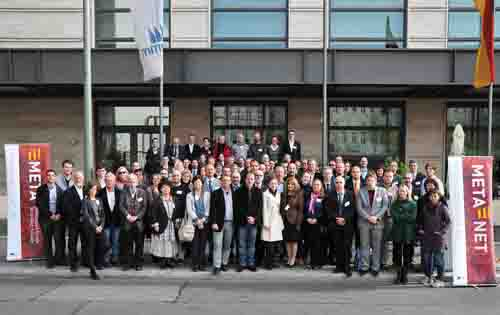
\includegraphics[width=\textwidth]{../_media/meta-net_team.jpg}
   \fbox{Dummy -- we'll include the group photo of our META-NET meeting in Berlin here}
  \caption{Rinne timpeall 100 saineolaí um theicneolaíocht teanga -- ionadaithe ó na tíortha agus teangacha atá i META-NET -- plé ar phríomhthorthaí agus teachtaireachtaí Shraith Páipéar Bán agus thug siad chun críche iad ag cruinniú i mBeirlín, an Ghearmáin, an 21/22~Deireadh Fómhair 2011. --- \textcolor{grey1}{About 100 language technology experts -- representatives of the countries and languages represented in META-NET -- discussed and finalised the key results and messages of the White Paper Series at a META-NET meeting in Berlin, Germany, on October 21/22, 2011.}} %NEEDS TO BE TRANSLATED
\end{figure*}

\cleardoublepage

\bsection[An Sraith Páipéar Bán META-NET -- The META-NET White Paper Series]{An Sraith Páipéar Bán META-NET --- The META-NET\ \ \ \ \ \ White Paper Series}
\label{whitepaperseries}

\vspace*{-5mm}
\centering
  \setlength{\tabcolsep}{2em}
  \begin{tabularx}{\textwidth}{lllll} \toprule\addlinespace
  %\begin{tabulary}{170mm}{LLL} \toprule
  &Bascais & Basque & euskara& \\
  &Béarla & English & English& \\
  &Bokmål Ioruais & Norwegian Bokmål & bokmål& \\
  &Bulgáiris & Bulgarian & български& \\
  &Catalóinis & Catalan & català& \\
  &Cróitis & Croatian & hrvatski& \\
  &Danmhairgis & Danish & dansk& \\
  &Eastóinis & Estonian & eesti& \\
  &Fionlainnis & Finnish & suomi& \\
  &Fraincis & French & français& \\
  &Gailísis & Galician & galego& \\
  &Gaeilge & Irish & Gaeilge& \\
  &Gearmáinis & German & Deutsch& \\
  &Gréigis & Greek & ελληνικά& \\
  &Iodáilis & Italian & italiano& \\
  &Íoslainnis & Icelandic & íslenska& \\
  &Laitvis & Latvian & latviešu valoda& \\
  &Liotuáinis & Lithuanian & lietuviu kalba& \\
  &Máltais & Maltese & Malti& \\
  &Nynorsk Ioruais & Norwegian Nynorsk & nynorsk& \\
  &Ollainnis & Dutch & Nederlands& \\
  &Polainnis & Polish & polski& \\
  &Portaingéilis & Portuguese & português& \\
  &Rómáinis & Romanian & româna& \\
  &Seirbis & Serbian & српски& \\
  &Seicis & Czech & ceština& \\
  &Slóvaicis & Slovak & slovencina& \\
  &Slóivéinis & Slovene & slovenšcina& \\
  &Spáinnis & Spanish & español& \\
  &Sualainnis & Swedish & svenska& \\
  &Ungáiris & Hungarian & magyar& \\ \addlinespace \bottomrule
\end{tabularx} %NEEDS TO BE TRANSLATED

\end{document}